%\documentclass[a4paper,oneside,12pt]{report} % n.pag scritto in basso
\documentclass[a4paper,oneside,11pt]{book}   
% Size and sheet settings
\usepackage[a4paper, top=3.5cm, bottom=3.5cm, left=2.5cm, right=3cm, heightrounded, bindingoffset=5mm]{geometry}

% Input encoding
\usepackage[utf8]{inputenc} 
% Per gestire le immagini
\usepackage{graphicx}  
% Per inserire margini laterali
\usepackage{scrextend} 
% Per fare la title page con immagine
\usepackage{titling}  
% For special styles (code)
\usepackage[dvipsnames]{xcolor}
\colorlet{punct}{red!60!black}
\definecolor{background}{HTML}{EEEEEE}
\definecolor{delim}{RGB}{20,105,176}
\colorlet{numb}{magenta!60!black}
\usepackage{listings}
\usepackage{code/jsonDD}
\usepackage{code/pseudocodeDD}

% To set depth table of contents
\setcounter{tocdepth}{4}

%% TABLES
% Utile per usare H per svuotare la cache dei floating objects come le table
\usepackage{float}     
% Necessario per rappresentare tabelle su più pagine
\usepackage{longtable} 
% Necessario per creare un nuovi tipi di colonna per le tabelle
\usepackage{array}     
\usepackage{tabu}

% Special table columns to center between cells
\newcolumntype{X}[1]{>{\centering\arraybackslash}p{#1}}
\newcolumntype{C}[1]{>{\centering\arraybackslash}m{#1}}
\newcolumntype{P}[1]{>{\arraybackslash}p{#1}}
\newcolumntype{H}[1]{>{\arraybackslash}m{#1}}

% Aggiunge funzionalità alle captions
\usepackage{caption}   
% Distacca le caption dalle table (verticalmente)
\captionsetup[table]{skip = 8pt} 
% Default: 6pt - Margine laterale  tra le celle delle tabelle
\setlength{\tabcolsep}{10pt}      
% Default: 1 - Margine verticale tra le celle delle tabelle
\renewcommand{\arraystretch}{1.7} 

% Multicolumn sections
\usepackage{multicol}

% Clickable references
\usepackage{hyperref} 
\hypersetup{
    colorlinks=true,
    linkcolor=blue,
    filecolor=black,      
    urlcolor=cyan,
    pdftitle={CLup - Design Document}, % Title of output file
    pdfpagemode=FullScreen,            % To open in fullscreen
}
% Command for two-part captions for tables/pictures
\newcommand{\captiondd}[2]{\caption{#1}\par\begin{center}\vspace{-.01\textheight}\small#2.\end{center}}
% Command for correctly spaced coloured text
\newcommand{\red}[1]{\begingroup\color{punct}#1\endgroup}

\title{\LARGE{DD -- Design Document}}
\author{Vincenzo Riccio, Giancarlo Sorrentino, Emanuele Triuzzi}
\date{January 10th, 2021}
\begin{document}

\begin{titlingpage} 
    \begin{center}
        
\includegraphics[height=0.52\linewidth]{pictures/polimi}\\ % Logo
        \begin{large}
            Software Engineering 2 \\
            A.Y. 2020-2021\\
        \end{large}
        \vspace{4cm} % Spaziatura verticale
        \begin{large} 
            \textbf{\thetitle} \\
        \end{large}
        \vspace{0.7cm}
        \theauthor\\
        \vspace{7.3cm} % Spaziatura verticale
        \thedate
    \end{center}
\end{titlingpage}

\newpage
\begin{table}[H]
    \begin{tabu} to \textwidth { X[0.3,r,p] X[0.7,l,p] }
        \hline
        \textbf{Deliverable:}   & DD\\
        \textbf{Title:}         & Design Document \\
        \textbf{Authors:}       & Vincenzo Riccio, Giancarlo Sorrentino, \newline Emanuele Triuzzi \\
        \textbf{Version:}       & 1.0 \\ 
        \textbf{Date:}          & January 10th, 2021 \\
        \textbf{Download page:} & https://github.com/SirGian99/RiccioSorrentinoTriuzzi \\
        \textbf{Copyright:}     & Copyright © 2021, Vincenzo Riccio, Giancarlo Sorrentino, Emanuele Triuzzi -- All rights reserved \\
        \hline
    \end{tabu}
\end{table}

\pagenumbering{roman}
\tableofcontents
\newpage
\pagenumbering{arabic}

\chapter{Introduction}
    \section{Purpose}
    CLup aims to provide chains of stores with a reliable solution to the problem of people gathering inside and outside the shops. \par
    To face the problem, the application focuses on its principal causes, which are the management of people inside the store, that often leads to overcrowding, the effectiveness of standard queuing systems and the way people are allowed to visit the stores. Moreover, the system aims to provide a useful tool for store managers in order to help them in administering stores and monitoring their status. \par
    In particular, the main goals that CLup aims to achieve, summarized in the table below, are the following:
    \begin{itemize}
        \item Prevent the store from being overcrowded, in order to avoid indoor gatherings while maximizing its occupancy, by means of an access management system;
        \item Reduce gatherings of people waiting to enter outside the store, providing a way to virtualize queues;
        \item Provide a more efficient way to access stores, reducing the time customers waste while waiting to do it;
        \item Help store managers in monitoring the status of the store and regulating the influx of people.
    \end{itemize}
    More details on how CLup is supposed to fulfill these goals are in the \href{run:../DeliveryFolder/RASD2.pdf}{Requirement Document}.
    
    \section{Scope}
    During the current situation of emergency, it is fundamental to prevent contacts among people. For this reason, governments impose strict rules concerning social distancing, both for indoor and outdoor contexts. \par
    However, crowding management inside stores like supermarkets and grocery shops could be challenging. Currently, stores limit the maximum number of people allowed, and therefore long queues arise: entering a store for a few minutes might even require hours. Moreover, customers who see a crowded store might avoid lining up to save time and prevent contact with others. \par
    CLup fits into this context allowing customers to remotely line-up in a queue of a given store and to be notified when they should head toward it. Furthermore, it allows the customer to book a visit for a store on a specific day and time, which grants him priority over the queued customers. \par
    Users can interact with CLup thanks to two distinct interfaces: one is an easy-to-use application designed for the customers, while the other one is an administrative tool that allows store managers to monitor their stores and modify their parameters. \par
    Moreover, CLup also manages physical proxies outside the stores as a fallback option for users who want to line-up but do not have access to the application.

    \section{Definitions, acronyms, abbreviations}
    \begin{longtable}[c] { |>{\bfseries{}}C{0.25\textwidth}|H{0.55\textwidth}| }
        \hline
        \multicolumn{2}{|c|}{\textbf{Definitions, acronyms, abbreviations}} \\
        \hline
        AMS                  & Access Management System \\ \hline
        TAS                  & Turn Announcement System \\ \hline
        CLup                 & Also known as the system. It is the software to be developed. From a design-oriented point-of-view, the term is also used to refer to the mobile application, the administrative tool and the server all together \\ \hline
        Customer application & Also known as application. It is used to access the functions provided by CLup  \\ \hline
        Administrative tool  & the tool provided to store managers in order to administer stores \\ \hline
        Proxy                & The physical fallback option for customers that want to use CLup but cannot use the application. It is placed outside the store it belongs to \\ \hline
        Turn Announcement System & An external system which informs customers about who has been allowed by CLup to enter the store it belongs to \\ \hline
        Access Management System & An external system which regulates physical entrances and exits to the store it belongs to by interacting with CLup \\ \hline
        App-customer & A customer who uses CLup functions through the application \\ \hline
        Proxy-customer & A customer who uses CLup functions through the proxy \\ \hline
        User & Either a customer or a store manager \\ \hline
        Long-term customer & With respect to a certain store, a customer who already used CLup to visit it \\ \hline
        Current occupancy & Also known as occupancy. It can be referred to the store or one of its sections. For the store, it is the number of people inside it. For the product sections, it is an index of the approximate number of people inside it the system can be aware of \\ \hline
        Maximum occupancy & Refers to the store or one of its sections. It is the maximum number of people allowed to be in that area \\ \hline
        Virtual queue & Also known as access queue or simply queue. It represents the set of customers who lined up through the app or the proxy \\ \hline
        Line-up & With respect to a customer and a store, it is the event of joining the queue \\ \hline
        Visit request & A customer’s request to visit a store. It can be either a line-up request or a booking request \\ \hline
        Line-up request & A request made by the customer to line-up for a store \\ \hline
        Booking request & A request made by the customer to book a visit to a store \\ \hline
        Visit & The realization of a visit request which takes place when a customer enters the store. After the customer exits the store, we talk about completed visit, otherwise it is a visit in progress  \\ \hline
        Visit token & A unique token bound to a visit request. It allows the Customer to enter and exit the store \\ \hline
        Pending request & A customer’s visit request that does not have a visit associated with and is not allowed to enter the store it is associated with \\ \hline
        Ready request & A customer’s visit request that does not have a visit associated with and is allowed to enter the store it is associated with \\ \hline
        Fulfilled request & A customer’s visit request that has an associated visit in progress \\ \hline
        Completed request & A customer’s visit request that has an associated completed visit \\ \hline
        Active request & A customer’s visit request that is not a completed request (thus it is either a pending, a ready or a fulfilled request) \\
        \hline
    \caption{Definition, acronyms, abbreviations}
    \label{table:definitions_acronyms_abbreviations}
    \end{longtable}

    \subsection{Revision history}
    1.0 -- First version of the document (January 10th, 2021).
    
    \section{Reference documents}
    \begin{itemize}
        \item IEEE standard for Software Design Descriptions, IEEE 1016-2009;
        \item R\&DD Assignment A.Y. 2020--2021;
        \item CLup Requirements Analysis and Specification Document (\href{run:../DeliveryFolder/RASD2.pdf}{RASD});
        \item Teaching material provided by professors Matteo Rossi and Elisabetta Di Nitto.
    \end{itemize}

    \section{Document structure}
    The reference structure used for the document is an adapted version of the one suggested by professor Matteo Rossi of Politecnico of Milan. \par It is derived from the IEEE standard, which is used as a reference document (IEEE standard for Software Design Descriptions, IEEE 1016-2009).
    \subsubsection{Chapter 1} 
    Chapter 1 is an introduction to the software to be designed and developed and to the problem that it addresses. It presents the goals that should be achieved and an analysis of the context in which the system will be placed.
    \subsubsection{Chapter 2} 
    Chapter 2 defines the system architecture. It includes a view of the system components and of their interfaces, a view about the deployment choices and some views about the runtime behaviour of the system. It also explains all the other design decisions.
    \subsubsection{Chapter 3} 
    Chapter 3 focuses on the design of the user interfaces. It also illustrates the users interactions with the system through mock-ups.
    \subsubsection{Chapter 4} 
    Chapter 4 better details the connections between goals and requirements already mapped in the RASD, taking into account the system components identified in Chapter 2
    \subsubsection{Chapter 5}
    Chapter 5 focuses on future plans about the implementation, the integration and the testing of the system components.
    \subsubsection{Chapter 6}
    Chapter 6 contains a report on the effort spent by all the members of the group while writing the current document.
    \subsubsection{Chapter 7}
    Last chapter contains references to the tools and resources used during the writing of this document.

\chapter{Architectural design}
    \section{Overview}
    The following sections are about the architecture of CLup. In order to better understand the whole document and to make it more self-contained, some recalls from the CLup Requirements Analysis and Specification Document follow, including an updated class diagram that considers a more design-oriented point-of-view.
    \begin{longtable}[c]{|>{\bfseries{}}c|H{.65\textwidth}|}
        \hline
        \multicolumn{2}{|c|}{\textbf{Functional requirements}} \\ \hline
        R1 & The system shall allow managers to specify the store parameters \\ \hline
        R2 & The system shall allow managers to monitor entrances \\ \hline
        R3 & The system shall allow managers to monitor exits \\ \hline
        R4 & The system shall authorize accesses to the store \\ \hline
        R4.1 & The system shall authorize customers to enter if and only if the store would not exceed the maximum number of people allowed inside it \\ \hline
        R5 & The system shall provide a way to line-up in the virtual queue of the store \\ \hline
        R6 & The system shall provide a way to exit the queue before entering the store \\ \hline
        R7 & The system shall alert the app-customer when it is time to reach the store \\ \hline
        R8 & The system shall provide the possibility to book a time interval for visiting the store \\ \hline
        R9 & The system must not allow customers to book a visit in a time interval if, over its duration, bookings by other users already maximize store occupancy \\ \hline
        R9.1 & The system must not allow customers to book a visit in a time interval if, over its duration, bookings by other users already maximize at least one of the product sections specified in the booking request \\ \hline
        R10 & When booking a visit, the system shall allow customers to specify what kind of products they intend to buy \\ \hline
        R11 & The system shall provide the possibility to cancel a booked visit before entering the store \\ \hline
        R12 & While making a booking request, the system shall suggest alternative time intervals if the demand of the chosen one is too high \\ \hline
        R13 & While making a booking request, the system shall suggest alternative stores of the same chain if the demand for the chosen time interval in the selected store is too high \\ \hline
        R14 & The system shall allow managers to regulate entrances \\ \hline
        R15 & The system shall allow managers to regulate exits \\ \hline
        R16 & The system shall notify a customer when, during a specific time interval, a specified store is reaching its maximum occupancy \\ \hline
        R17 & The system shall keep track of the average duration of a generic visit to the store \\ \hline
        R18 & The system shall manage the case in which customers do not show up when it is their turn to enter the store \\ \hline
        R19 & The system shall inform customers when they are allowed to enter the store \\ \hline
        \caption{Functional requirements}
        \label{table:functional_requirements}
    \end{longtable}
    
    \newpage
    \begin{longtable}[c]{|>{\bfseries{}}c|H{.65\textwidth}|}
        \hline
        \multicolumn{2}{|c|}{\textbf{Non-functional requirements}} \\ \hline
        \hypertarget{NF1}{NF1} & The system, in normal operating conditions, should be able to handle all line-up and booking requests of each customer \\ \hline
        NF2 & The system responses and notifications must be sent within 3 seconds from the triggering event \\ \hline
        NF3 & The software should be GDPR compliant \\ \hline
        NF4 & CLup should provide a high degree of reliability \\ \hline
        \hypertarget{NF5}{NF5} & CLup should be available the 99\% of the time \\ \hline
        \hypertarget{NF6}{NF6} & The system should be protected against malicious attacks \\ \hline
        NF7 & The system must be well-documented and adaptable to changes \\ \hline
        NF8 & The CLup customer application should be compatible with most of the smartphones currently on the market \\ \hline
        NF9 & CLup should be platform independent \\ \hline
        NF10 & The application should be easy to use \\ \hline
        NF11 & CLup shall give priority to booking requests over line-up requests \\ \hline
        NF12 & Customers can remotely line-up in a store’s queue only if they are not in the queue of any store at that moment \\ \hline
        NF13 & Customers can book a visit to a store for a specific time interval only if they have not booked any other visit which overlaps with that time interval \\ \hline
        NF14 & Customers can book a visit to a store for a specific time interval only if it starts after the current queue disposal time of that store \\ \hline
        \caption{Non-functional requirements}
        \label{table:non_functional_requirements}
    \end{longtable}

    \begin{figure}[H]
        \centering
        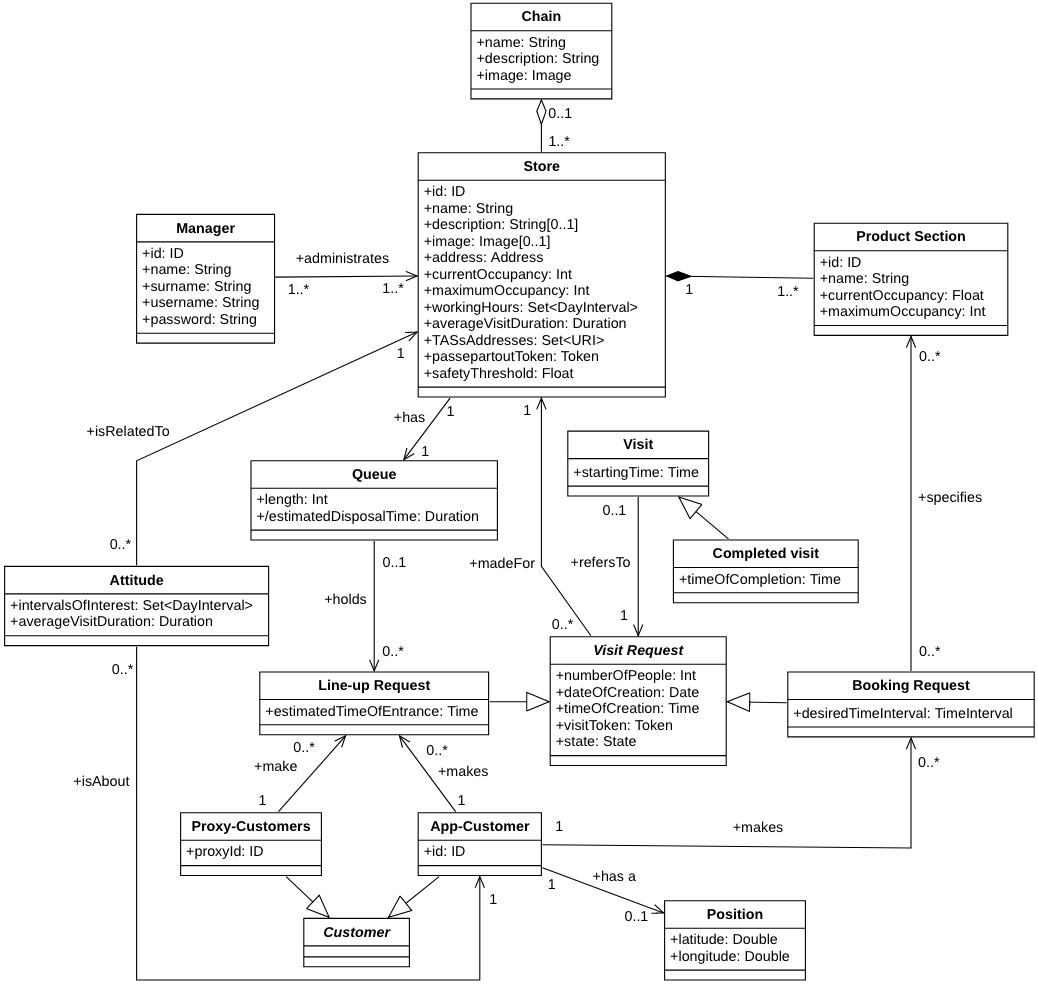
\includegraphics[width=\textwidth, height=\textheight, keepaspectratio]{pictures/uml_class_diagram}
        \caption{UML Class Diagram}
        \label{figure:uml}
    \end{figure}
    For the sake of simplicity and readability of the diagram, complex types of attributes are detailed below and not included in the diagram itself. 
    \begin{figure}[H]
        \centering
        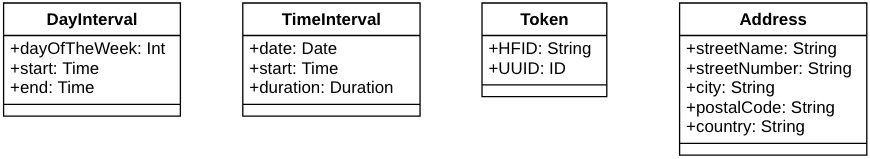
\includegraphics[width=.8\textwidth, height=\textheight, keepaspectratio]{pictures/uml_complex_attributes}
        \caption{UML complex attributes}
        \label{figure:uml_complex_attributes}
    \end{figure}
    Furthermore, \textit{Image} and \textit{Duration} are abstract types representing respectively an image and a time duration, while \textit{State} is an enumeration of the possible states of a request (pending, ready, fulfilled, completed). \par
    Since the system does not provide other functions to proxy customers other than the one to make line-up requests for the store the proxy belongs to, and since proxies are not intended to identify customers, it has been decided to consider all the customers interacting with a single proxy as the same instance of ``\textit{Proxy Customers}". \par
    Details on the attribute mentioned are provided through the following sections. \par
    As evidenced by the following sections, CLup is modelled according to a multi-tier 3-layer architecture. The software components to be developed are the server, the mobile application and the administrative tool, which in the current document are mentioned all together as CLup or system.
    
    \subsection{Selected architectural styles and patterns}
    The whole system (i.e. CLup itself) is designed as a multi-tier 3-layer architecture. Thus, it allows the decoupling of presentation, logic and data layers, which are hosted on different devices.
    \begin{itemize}
        \item The \textbf{presentation layer} includes all the devices which customers and managers interact with in order to use the services offered by CLup;
        \item The \textbf{application} (logic) \textbf{layer} includes all the components needed to guarantee the complete implementation of CLup functions;
        \item The \textbf{data layer} includes the DBMS in charge of managing all the persistent data of CLup.
    \end{itemize}
    As can be seen from the class diagram, all the classes use structured data and have many associations between them. Furthermore, the persistent storage has not to deal with a huge amount of data. Hence the decision to opt for a relational database. \par
    The application layer also includes third-part components which the system interacts with and which allow it to properly offer its services. \par
    The only noticeable exception in the CLup 3-layer architecture is represented by the interaction between the mobile application and the NotificationService component. Indeed, the MobileApplication offers an interface, which depends on the development technology stack, that guarantees the feasibility of remote push notifications service offered by CLup. More details on this design choice are provided in Section  \ref{section:design_decisions}. \par
    The interfaces between the presentation layer and the application layer are designed according to the REST (Representational State Transfer) architectural style and are based on the HTTPS protocol. Thus, each interaction between those layers is stateless and follows a client-server approach. \par
    Since REST applies the ``separation of concerns" (SoC) paradigm, it allows an independent development and replacement of both the client-side logic and the server-side logic as long as the interfaces are not changed. \par
    Furthermore, this choice results in an improvement of the portability (and the freedom of implementation choices) of the user interfaces across multiple platforms, of the scalability of the system (by simplifying the server components) and of the maintainability. \par
    Regarding the functionalities that involve the notification of app-customers, it was decided to use existing providers of remote push notifications. \par
    No constraints concerning the provider of the push notification service (e.g. Google Firebase, Apple Push Notification service) and the one of the maps service (e.g. Google Maps, OpenStreetMap) are imposed on the developers. Thus, across the entire document, the NotificationService component and the MapsService component are considered as dependent on the chosen service provider. \par
    While the server, the mobile application and the administrative tool are the software components to be developed:
    \begin{itemize}
        \item the proxy and the AMS are existing components that will be configured to interact with the system through the interfaces provided by CLup. Thus, they are supposed to be able to communicate with CLup over HTTPS;
        \item the TAS, the NotificationService and the MapsService components are existing components which CLup interacts with through the interfaces they provide. They all offer an interface through the HTTPS protocol;
        \item Also the DBMS component is an existing component which offers an interface to CLup. Their communication is based on TCP/IP.
    \end{itemize}
    In order to reach a low level of coupling, the server internal logic has been the object of a functional decomposition into sub-components and has been designed considering the proxy design pattern when dealing with external components. Indeed, as can be seen from the component diagram presented in the following section, the PushNotificationController and the MapController components act as interfaces respectively to the external NotificationService and MapsService components.
 \par
    Furthermore, the DataModel component, which also acts as an interface to the data storage, represents the repository of the homonym pattern. \par
    Further details on the components and on their interactions follow.
    
    \newpage
    \section{Component view}
    \subsection{High-level component view}
    \begin{figure}[H]
        \centering
        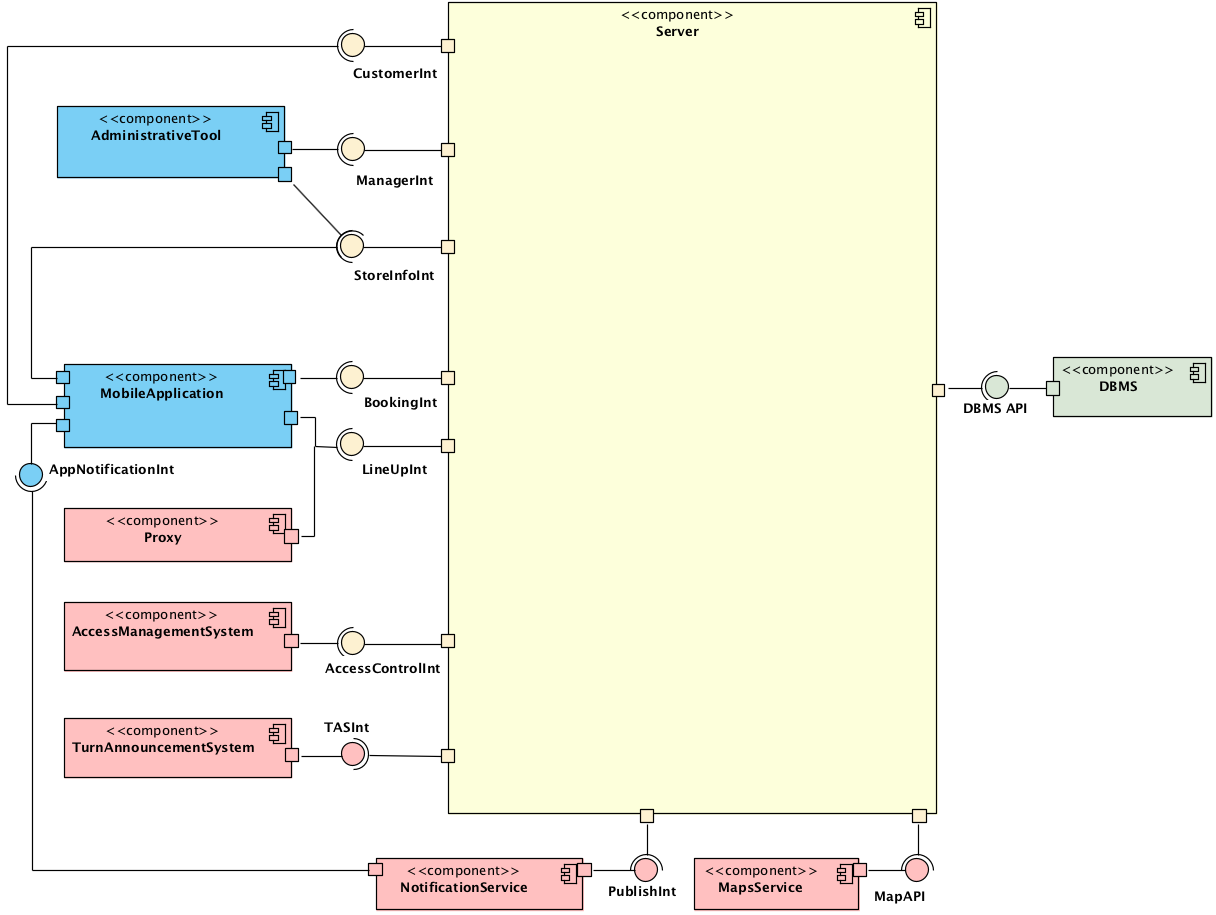
\includegraphics[width=\textwidth, height=\textheight, keepaspectratio]{pictures/component_diagram_hl}
        \captiondd{Component diagram}{This high level component view provides an overview of the 3-layer architecture, and highlights the different interfaces which allow the components to interact with the system}
        \label{figure:component_diagram_hl}
    \end{figure}
    
    \subsection{Detailed component view}
    \begin{figure}[H]
        \centering
        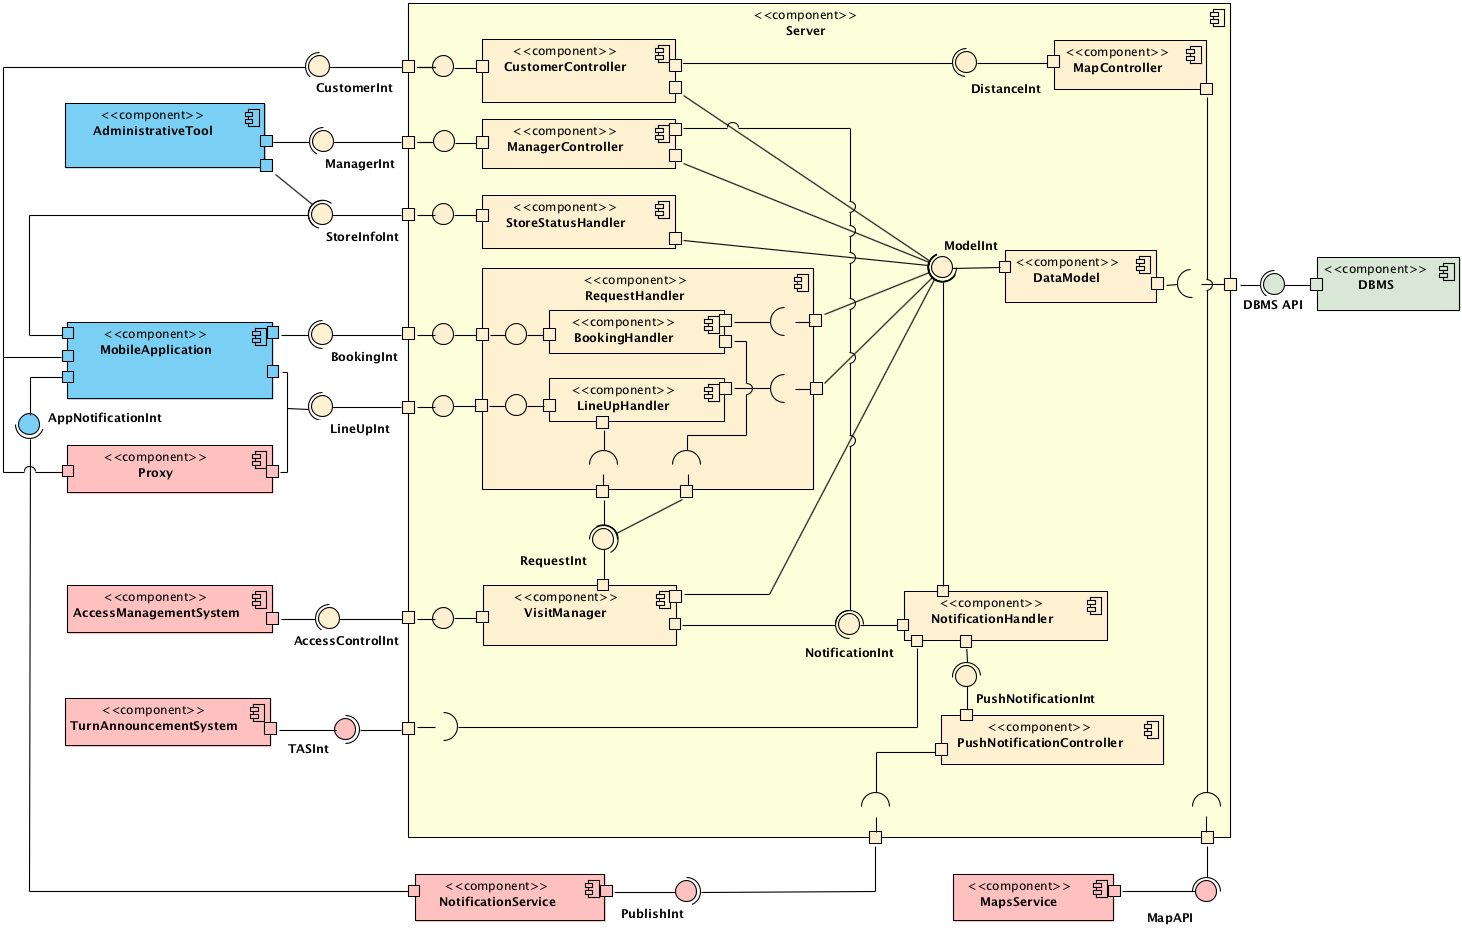
\includegraphics[width=\textwidth, height=\textheight, keepaspectratio]{pictures/component_diagram_exp}
        \caption{Detailed component diagram}
        \label{figure:component_diagram_exp}
    \end{figure}
    
    \subsection{Components description}
    \subsubsection{High-level components}
    \begin{itemize}
        \item \textbf{MobileApplication}: it is the smartphone application used by customers to interact with CLup. In order to allow customers to use all the functions provided by the system, it interacts with the server as a client via several interfaces. It also offers an interface to the NotificationService that allows CLup to send remote notifications to the customer.
        \item \textbf{AdministrativeTool}: it is the desktop application used by store managers in order to monitor and administer their stores.
        \item \textbf{Proxy}: it is the component that provides a fallback option to customers who cannot use the MobileApplication. Each instance of this component is associated with a single store managed by CLup and allows customers to line-up in the store’s queue.
        \item \textbf{AccessManagementSystem}: the component in charge of letting customers enter and exit the stores with respect to their visit token. Each instance of this component is associated with a single store managed by CLup, and contacts the VisitManager via the AccessControlInterface to determine whether a customer is allowed to enter the store. \par 
        It also informs CLup when the customer actually enters and exits the store, specifying how many people actually enter and exit it.
        \item \textbf{TurnAnnouncementSystem}: the component in charge of informing customers outside the stores when they are allowed to enter the store. Each instance of this component is associated with a single store managed by CLup and provides an interface to be notified whenever a new customer is allowed to enter the store. It can also provide information about the store’s queue disposal time, its length, or the average duration of a visit in its store.
        \item \textbf{NotificationService}: it is the external component which manages the dispatching of push notifications to the MobileApplication. It offers an interface to the CLup in order to collect notifications, and sends them to the MobileApplication of the receiver. 
        \item \textbf{MapsService}: it is the external component used to perform the geo-spatial requests made by CustomerController component. It provides an interface contacted by the MapController, which mediates between the two components.
        \item \textbf{Server}: it is the component implementing the system logic.
    \end{itemize}
    \subsubsection{Internal server components}
    \begin{itemize}
        \item \textbf{RequestHandler}: the component is the one in charge of collecting customers’ visit requests, accepting or rejecting them, and of cancelling the same requests whenever the customer who placed them asks for it. The request handler is composed of two sub components:
        \begin{itemize}
            \item \textbf{LineUpHandler}: the component in charge of collecting, accepting and rejecting line-up requests made by all customers. When a request is accepted, the LineUpHandler informs the DataModel and notifies the VisitManager via its dedicated interface. The rejection is performed taking into account the status of the store they refer to, retrieved from the DataModel. This component is also the one in charge of dealing with customers’ requests to cancel their previously made line-up requests, informing the DataModel and notifying the VisitManager.
            \item \textbf{BookingHandler}: the component in charge of collecting, accepting and rejecting booking requests made by app-customers. It also balances out the affluence to the desired store in each time interval. To do so, when a request is placed, if the store is likely to reach its maximum occupancy in the specified time interval, before accepting it the component suggests alternative time intervals to the customer. When a request is accepted, the component informs the DataModel and notifies the VisitManager via its dedicated interface. A request is rejected taking into account the status of the store it refers to in the specified time interval, retrieved from the DataModel. When this happens, the BookingHandler is also in charge of suggesting the customer alternative time intervals or stores of the same chain in which to perform the booking. \par 
            This component is also the one which deals with customers’ requests to cancel their previously made booking requests, informing the DataModel and notifying the VisitManager. \par
            Moreover, the BookingHandler is in charge of providing customers with information about the estimated time of entrance associated with their booking request if it is the booking desired time but the customer is not allowed yet to enter the store.  
        \end{itemize}   
        \item \textbf{CustomerController}: the component in charge of retrieving and providing app-customers with their information, such as their active line-up and booking requests. It also manages customers’ requests to be notified about stores becoming unavailable in some specific day intervals. These day intervals can both be specified by the customer or automatically inferred by the component, based on the previous customers’ visits to the selected store. Moreover, for each app-customer, it periodically makes an estimation on the average duration of a visit in each store already visited by each app-customer.\par
        Furthermore, it informs app-customers when they should start heading to the store they lined-up for in order to arrive on time. To do so, it periodically receives the current position of a customer and delegates the MapController component to get the time he would need in order to reach the store he lined-up for by walk and by car.
        \item \textbf{ManagerController}: the component in charge of handling with managers authentication and providing them with information about their profile, such as the list of stores they manage. Furthermore, it is the component in charge of allowing managers to administer their stores, modifying their relative parameters. When it is needed to inform some customers about a performed change, it notifies their MobileApplication by contacting the NotificationHandler (more details are provided in section \ref{section:design_decisions}). Moreover, the ManagerController component is also the one in charge of allowing store managers to add already existing managers to their stores, or even add new ones.
        \item \textbf{StoreStatusHandler}: this component is the one in charge of providing all the information concerning the stores managed by CLup, such as their opening time, their current occupancy, their product sections and relative occupancies, their current queue disposal time. Also, it periodically estimates and updates the average duration of a visit to each store.
        \item \textbf{VisitManager}: this component is the one in charge of coping with visits and visit requests to the stores managed by CLup. In fact, it regulates the order in which customers are allowed to visit the stores they made visit requests for, and also manages the situation in which customers do not show up when it is their turn. Moreover, when a visit request is in its ready state, it communicates this information to the NotificationHandler via its dedicated interface. The VisitManager also provides an interface to allow entrances and exits to the stores managed by CLup, by checking if given a visit token and a store the token is associated with a visit request in ready state for the selected store. In addition, this component is the one in charge of informing the NotificationHandler when a given store is likely to reach its maximum occupancy. 
        \item \textbf{NotificationHandler}: this component is the one in charge of notifying customers when they are allowed to enter the store. When this happens, the NotificationHandler contacts the TurnAnnouncementSystem, providing it with the visit tokens of the ready requests and with other information about the store. Moreover, in case of visit requests placed by app-customers, the NotificationHandler interacts with the PushNotificationController in order to send remote push notifications to the customers’ mobile application. \par
        The NotificationHandler is also in charge of notifying app-customers whenever the stores they asked to be notified about are likely to reach their maximum occupancy in a given day interval. In fact, when a store is reaching its maximum occupancy in a certain day interval, the NotificationHandler, which has been informed by the VisitManager about that event, retrieves from the DataModel the app-customers to be notified and eventually notifies them via the PushNotificationController.
        \item \textbf{PushNotificationController}: this component is the one in charge of mediating between the system and the NotificationService. It receives requests from the NotificationHandler that include the identifier of the app-customer to be notified and the content of the notification. It then forwards the request to the NotificationService.
        \item \textbf{MapController}: this component is the one in charge of mediating between the system and the MapsService. In fact, it receives geo-spatial requests from the CustomerController component and performs them exploiting the MapsService. 
        \item \textbf{DataModel}: this component is the one that defines the data model of the system and interacts with the DBMS in order to ensure data persistence. All the other components of the system interact with it in order to read and update data. 
    \end{itemize}
    
    \newpage
    \section{Component interfaces}
    \subsection{CLup RESTful interfaces}
    The interfaces between the presentation layer and the application layer are designed considering the REST architectural style upon the HTTPS protocol. All the request/response bodies are encoded using the JSON format. VALUE is the symbolic token representing the value provided in the request/response message body. \par
    Thus, these interfaces form a RESTful API.
    
    \subsubsection{ManagerInt}
    It is the interface provided by the ManagerController. It is used by the AdministrativeTool in order to allow a manager to administer his stores. Thus, all the operations initiated by a certain manager and related to a certain store are performed only if that store is administered by that manager and applied by the system when the store is closed. The interface includes:
    \begin{longtable}[c] { |>{\centering\arraybackslash}P{0.11\textwidth}|>{\centering\arraybackslash\ttfamily}H{0.23\textwidth}|H{0.50\textwidth}| }
        \hline
        \textbf{HTTP verb} & \textrm{\textbf{URI}} & \textbf{\textbf{Description}} \\ \hline
        POST & /manager/login & It allows a manager to initiate a session starting from a login. The request body has the following structure: 
        \begin{lstlisting}[language=jsonDD]
{
 "username" : "VALUE",
 "password" : "VALUE"
}
        \end{lstlisting}
        The response body has the following structure:
        \begin{lstlisting}[language=jsonDD]
{
 "managerID" : "VALUE",
 "authenticationToken": "VALUE"
}
        \end{lstlisting}
        Further details on the authentication token are provided in section \ref{section:design_decisions} \\ \hline
        GET & /manager/\{id\}/ logout & It allows a manager to logout and to invalidate the authentication token \\ \hline
        GET & /manager/\{id\} & It returns the general information of the manager identified by the parameter \texttt{\{id\}} plus the basic information about the stores he manages. The response body has the following structure:
        \begin{lstlisting}[language=jsonDD]
{
  "username": "VALUE",
  "name": "VALUE",
  "surname" : "VALUE",
  "stores" : [
     {"id" : "VALUE",
      "chain" : "VALUE",
      "name" : "VALUE",
      "address" : "VALUE"}, 
      ...
   ]
}
        \end{lstlisting} \\ \hline
        POST & /manager/\{id\}/ newManager & It creates a new manager for a store. The manager identified by \texttt{\{id\}} is the responsible for the operation. The request body has the following structure:
        \begin{lstlisting}[language=jsonDD]
{
  "newUsername": "VALUE",
  "newPassword": "VALUE",
  "name": "VALUE",
  "surname" : "VALUE",
  "storeID" : "VALUE"
}
        \end{lstlisting} \\ \hline
        POST & /manager/\{id\}/ addManager & It adds an existing manager to a store. The manager identified by \texttt{\{id\}} is the responsible for the operation. The request body has the following structure:
\begin{lstlisting}[language=jsonDD]
{
  "newManagerUsername": "VALUE",
  "storeID" : "VALUE"
}
\end{lstlisting} \\ \hline
        POST & /manager/\{id\}/ removeManager & It removes an existing manager to a store. The manager identified by \texttt{\{id\}} is the responsible for the operation. The request body has the following structure:
\begin{lstlisting}[language=jsonDD]
{
  "managerToRemoveUsername": "VALUE",
  "storeID" : "VALUE"
}
\end{lstlisting} \\ \hline
        PATCH & /manager/\{id\}/ store/\{storeID\} & It modifies the store identified by the parameter \texttt{\{storeID\}}. The manager identified by {id} is the responsible for the operation. As detailed in section \ref{section:design_decisions}, it may have an impact on customers’ visit requests. The parameters which will be modified are the ones in the request body, which admits the following parameters:
\begin{lstlisting}[language=jsonDD]
"name" : "VALUE"
"address" :  {
     "streetName" : "VALUE",
     "streetNumber" : "VALUE",
     "city" : "VALUE",
     "postalCode" : "VALUE",
     "country" : "VALUE"
 }
"workingHours" : [
   {"day" : "VALUE",
    "start": "VALUE",
    "end": "VALUE"},
    ...
]
"maximumOccupancy" : "VALUE"
"safetyThreshold" : "VALUE"
\end{lstlisting} 
        As detailed in section \ref{section:design_decisions}, the maximum occupancy of a store is specified (and can be modified) by the manager only when the store is not divided in product sections \\ \hline
        PUT & /manager/\{id\}/ store/\{storeID\}/ addSection & It adds a new section to the store identified by the parameter \texttt{\{storeID\}}. The manager identified by \texttt{\{id\}} is the responsible for the operation. The request body has the following structure:
\begin{lstlisting}[language=jsonDD]
{
  "name" : "VALUE",
  "maximumOccupancy" : "VALUE"
}
The response body has the following structure:
{
  "sectionID" : "VALUE"
}
\end{lstlisting} \\ \hline
        PATCH & /manager/\{id\}/ store/\{storeID\}/ section/ \{sectionID\} & It modifies the section with id \texttt{\{sectionID\}} of the store identified by the parameter \texttt{\{storeID\}}. The manager identified by {id} is the responsible for the operation. As detailed in section \ref{section:design_decisions}, it may have an impact on customers’ visit requests. The parameters which will be modified are the ones in the request body, which admits the following parameters:
\begin{lstlisting}[language=jsonDD]
"name" : "VALUE",
"maximumOccupancy" : "VALUE"
\end{lstlisting} \\ \hline
        DELETE & /manager/\{id\}/ store/\{storeID\}/ section/ \{sectionID\} & It deletes the section with id \texttt{\{sectionID\}} of the store identified by the parameter \texttt{\{storeID\}}. The manager, identified by \texttt{\{id\}}, is the responsible for the operation. As detailed in section \ref{section:design_decisions}, it may have an impact on customers’ visit requests
        \\ \hline
        GET & /manager/\{id\}/ store/\{storeID\}/ passepartout & It returns the passepartout token of the store identified by \texttt{\{storeID\}}. The manager, identified by \texttt{\{id\}}, is the responsible for the operation. The response body has the following structure:
        \begin{lstlisting}[language=jsonDD]
{
  "hfid" : "VALUE",
  "uuid" : "VALUE"
}
        \end{lstlisting} \\ \hline
        \caption{ManagerInt}
        \label{table:manager_int}
    \end{longtable}
    
    \subsubsection{CustomerInt}
    It is the interface provided by the CustomerController. It is used by the MobileApplication to interact with the system. Furthermore, it is used by the Proxy to perform its registration in the system. The interface includes:
    \newpage
    \begin{longtable}[c] { |>{\centering\arraybackslash}P{0.11\textwidth}|>{\centering\arraybackslash\ttfamily}H{0.23\textwidth}|H{0.50\textwidth}| }
        \hline
        \textbf{HTTP verb} & \textrm{\textbf{URI}} & \textbf{\textbf{Description}} \\ \hline
        PUT & /customer/ registerProxy & It allows the (automatic) registration of a new proxy. The request body has the following structure: 
        \begin{lstlisting}[language=jsonDD]
{
   "proxyID" : "VALUE"
}
        \end{lstlisting} Details about the proxy id in section \ref{section:design_decisions} \\ \hline
        PUT & /customer/ registerApp & It allows the (automatic) registration of a new app-customer at the first launch of the app. The request body has the following structure:
        \begin{lstlisting}[language=jsonDD]
{
   "appID" : "VALUE"
}
        \end{lstlisting} Details about the app id in section \ref{section:design_decisions} \\ \hline
        GET & /customer/\{id\} & It returns all the active visit requests of the customer identified by \texttt{\{id\}}. The response body has the following structure:
        \begin{lstlisting}[language=jsonDD]
{
   "lineupRequest" : {
        "visitToken" : {
            "hfid" : "VALUE",
            "uuid" : "VALUE"
         },
        "storeID" : "VALUE"
        "numberOfPeople" : "VALUE",
        "estimatedTimeOfEntrance" : "VALUE"
   },
  "bookingRequests" : [
        {"visitToken" : {
            "hfid" : "VALUE",
            "uuid" : "VALUE"
          }
         "storeID" : "VALUE"
         "numberOfPeople" : "VALUE",
         "desiredTimeInterval" : {
             "date" : "VALUE",
             "start" : "VALUE",
             "duration" : "VALUE"
          },
         "productSectionsNames": ["VALUE", ...]
        },
        ...
   ]
}
        \end{lstlisting} \\ \hline
        POST & /customer/\{id\}/ askForNotification & It adds the customer to the ones that want to be notified when the selected store is likely to become unavailable. The request body has then the following structure:
        \begin{lstlisting}[language=jsonDD]
{
   "auto" : "VALUE",
   "store": "VALUE",
   "dayIntervals": [
       {
          "dayOfTheWeek": "VALUE",
          "start": "VALUE",
          "end": "VALUE"
       }, 
    ...
   ]
}
        \end{lstlisting} If the day intervals are specified by the customer, the auto parameter must be set to ``\texttt{False}". Otherwise, it is set to ``\texttt{True}" and the day intervals should not be specified \\ \hline
        POST & /customer/\{id\}/ updatePosition & It checks if the customer identified by the specified token should head towards the store he lined up for, according to his actual position. The request body has the following structure:
        \begin{lstlisting}[language=jsonDD]
{
   "latitude" : "VALUE",
   "longitude" : "VALUE"
}
        \end{lstlisting} 
         The response body has the following structure:
        \begin{lstlisting}[language=jsonDD]
{
   "shallNotify" : "VALUE",
   "estimatedTimeWalking" : "VALUE",
   "estimatedTimeDriving" : "VALUE"
}
        \end{lstlisting} 
        \\ \hline
        GET & /customer/\{id\}/ store/\{storeID\}/ averageDuration & It returns the average duration of a visit to the selected store of the specified customer. The response body has the following structure: 
        \begin{lstlisting}[language=jsonDD]
{
  "averageDuration" : "VALUE"
}
    
        \end{lstlisting} \\ \hline
        \caption{CustomerInt}
        \label{table:customer_int}
    \end{longtable}
    
    \subsubsection{StoreInfoInt}
    It is the interface provided by the StoreStatusHandler. It is used by the AdministrativeTool and by the MobileApplication in order to retrieve information about a store or a chain, plus the list of all the chains managed by the system. The interface includes:
    \begin{longtable}[c] { |>{\centering\arraybackslash}P{0.11\textwidth}|>{\centering\arraybackslash\ttfamily}H{0.23\textwidth}|H{0.50\textwidth}| }
        \hline
        \textbf{HTTP verb} & \textrm{\textbf{URI}} & \textbf{\textbf{Description}} \\ \hline
        GET &/manager/\{id\}/ generalInfo & It returns general information about the store identified by the parameter \texttt{\{id\}}. The response body has the following structure:
        \begin{lstlisting}[language=jsonDD]
{  
  "chainName" : "VALUE",
  "name" : "VALUE",
  "address" : {
      "streetName" : "VALUE",
      "streetNumber" : "VALUE",
      "city" : "VALUE",
      "postalCode" : "VALUE",
      "country" : "VALUE"
   },
  "description" : "VALUE",
  "image" : "VALUE",
  "currentOccupancy" : "VALUE",
  "maximumOccupancy" : "VALUE",
  "safetyThreshold" : "VALUE"
  "averageVisitDuration" : "VALUE",
  "queueLength" : "VALUE",
  "queueDisposalTime" : "VALUE",
  "workingHours" : [
     {"day" : "VALUE",
      "start": "VALUE",
      "end": "VALUE"},
    ...
   ]
}
        \end{lstlisting} \\ \hline
        GET & /store/\{id\}/ activeRequest & It returns all the active requests associated with the store identified by the parameter \texttt{\{id\}}. The response body has the following structure:
        \begin{lstlisting}[language=jsonDD]
{
  "lineupRequests" : [
     {"customerID" : "VALUE",
      "timeOfCreation" : "VALUE",
      "numberOfPeople" : "VALUE",
      "visitToken" : {
          "hfid" : "VALUE",
          "uuid" : "VALUE"
       },
      "state" : "VALUE",
      "estimatedTimeOfEntrance" : "VALUE",
      "startingTime" : "VALUE",
      "isFromProxy": "VALUE"},
     ...
  ],
  "bookingRequests" : [
     {"customerID" : "VALUE",
      "desiredTimeInterval" : {
          "date" : "VALUE",
          "start" : "VALUE",
          "duration" : "VALUE"
       },
      "numberOfPeople" : "VALUE",
      "visitToken" : {
          "hfid" : "VALUE",
          "uuid" : "VALUE"
       },
      "state" : "VALUE",
      "sectionsIDs" : ["VALUE", ...] },
     ...
  ]
}
        \end{lstlisting} 
       ``\texttt{isFromProxy}" is a boolean value which indicates whether the line-up request was placed using a proxy or the application\\ \hline
        GET & /store/\{id\}/ managers & It returns the managers of the store identified by the parameter \texttt{\{id\}}. The response body has the following structure:
        \begin{lstlisting}[language=jsonDD]
{
  "managers" : [
     {"username": "VALUE",
      "name": "VALUE",
      "surname" : "VALUE"}, 
    ...
   ]
}
        \end{lstlisting} \\ \hline
        GET & /store/\{id\}/ sections & It returns the sections of the store identified by the parameter {id}. The response body has the following structure:
        \begin{lstlisting}[language=jsonDD]
{
  "sections" : [
     {"id": "VALUE",
      "name": "VALUE",
      "currentOccupancy" : "VALUE",
      "maximumOccupancy" : "VALUE"}, 
    ...
   ]
}
        \end{lstlisting} \\ \hline
        GET & /chainstore? city=value & It returns all the available chains and independent stores in the specified city. If the city is not specified, it returns all the chains managed by CLup. The response body has the following structure:
        \begin{lstlisting}[language=jsonDD]
{
  "chains" : [
     {"name": "VALUE",
      "description" : "VALUE",
      "image" : "VALUE"}, 
    ...
   ],
 "autonomousStores" :  [
     {"name": "VALUE",
      "description" : "VALUE",
      "image" : "VALUE"}, 
    ...
   ]
}
        \end{lstlisting} \\ \hline
                GET & /chain/\{name\}/ stores?city=value & It returns the identifier, the name and the address of all the stores of the selected chain. If the city parameter is specified, the results are limited to the stores located in that city. The response body has the following structure:
        \begin{lstlisting}[language=jsonDD]
{
   "stores" : [
    {"id" : "VALUE",
     "name" : "VALUE",
      "address" : {
          "streetName" : "VALUE",
          "streetNumber" : "VALUE",
          "city" : "VALUE",
          "postalCode" : "VALUE",
          "country" : "VALUE"}
    },
    ...
   ]
}
        \end{lstlisting} \\ \hline
        \caption{StoreInfoInt}
        \label{table:storeinfo_int}
    \end{longtable}
    
    \subsubsection{LineUpInt}
    It is an interface provided by the LineUpHandler. It is used by the Proxy and by the MobileApplication in order to allow a customer to line-up for a specific store. It also allows an app-customer to delete a pending request and to check approximately how long it takes for being allowed to enter the store he lined-up for. The interface includes:
    \begin{longtable}[c] { |>{\centering\arraybackslash}H{0.11\textwidth}|>{\centering\arraybackslash\ttfamily}P{0.23\textwidth}|H{0.50\textwidth}| }
        \hline
        \textbf{HTTP verb} & \textrm{\textbf{URI}} & \textbf{\textbf{Description}} \\ \hline
        POST & /lineup & It checks if a certain line-up request is feasible and, if so, it accepts the request. The request body has the following structure:
        \begin{lstlisting}[language=jsonDD]
{
   "storeID" : "VALUE",
   "numberOfPeople" : "VALUE",
   "customerID" : "VALUE"
}
        \end{lstlisting}
        The response body has the following structure:
        \begin{lstlisting}[language=jsonDD]
{
   "validated" : "VALUE",
   "estimatedTimeOfEntrance" : "VALUE",
   "visitToken" : {
          "hfid" : "VALUE",
          "uuid" : "VALUE"
    }
}
        \end{lstlisting}  \\ \hline
        DELETE & /lineup/\{token\} & It deletes a pending or a ready line-up request which is identified by \texttt{\{token\}} \\ \hline
        \caption{LineUpInt}
        \label{table:lineup_int}
    \end{longtable} 
    
    \newpage
    \subsubsection{BookingInt}
    It is an interface provided by the BookingHandler. It is used by the MobileApplication in order to allow a customer to request or delete a booking for a certain store. The interface includes:
    \begin{longtable}[c] { |>{\centering\arraybackslash}H{0.11\textwidth}|>{\centering\arraybackslash\ttfamily}P{0.23\textwidth}|H{0.50\textwidth}| }
        \hline
        \textbf{HTTP verb} & \textrm{\textbf{URI}} & \textbf{\textbf{Description}} \\ \hline
        POST & /booking & It checks if a certain booking request is feasible and, if so, it accepts the request. The request body has the following structure:
        \begin{lstlisting}[language=jsonDD]
{
   "storeID" : "VALUE",
   "numberOfPeople" : "VALUE",
   "customerID" : "VALUE",
   "desiredTimeInterval" : {
       "date" : "VALUE",
       "start" : "VALUE",
       "duration" : "VALUE"
    },
   "sectionsIDs" : ["VALUE", ...],
   "alternativesDesired" : "VALUE"
}
        \end{lstlisting}
        The response body has the following structure:
        \begin{lstlisting}[language=jsonDD]
{
   "validated" : "VALUE",
   "visitToken" : {
       "hfid" : "VALUE",
       "uuid" : "VALUE"
    },
   "alternativeTimeIntervals" : [
     {"date" : "VALUE",
      "start" : "VALUE",
      "duration" : "VALUE"},
      ...
    ],
   "alternativeStores" : [
     {"id" : "VALUE",
      "name" : "VALUE",
      "address" : {
         "streetName" : "VALUE",
         "streetNumber" : "VALUE",
         "city" : "VALUE",
         "postalCode" : "VALUE",
         "country" : "VALUE"
      }},
      ...
   ]
}
        \end{lstlisting}
        Alternatives are in the response only if \texttt{alternativesDesired} parameter is \texttt{true}
        \\ \hline
        DELETE & /booking/\{token\} & It deletes the pending booking request identified by \texttt{\{token\}} \\ \hline
        \caption{BookingInt}
        \label{table:booking_int}
    \end{longtable}
    
    \subsubsection{AccessControlInt}
    It is an interface provided by the VisitManager. It is used by the AccessManagementSystem in order to check if a customer of the store it belongs to is allowed to access that store. The interface includes:
    \begin{longtable}[c] { |>{\centering\arraybackslash}H{0.11\textwidth}|>{\centering\arraybackslash\ttfamily}P{0.23\textwidth}|H{0.50\textwidth}| }
        \hline
        \textbf{HTTP verb} & \textrm{\textbf{URI}} & \textbf{\textbf{Description}} \\ \hline
        POST & /access/request & It checks if the customer associated with the token provided in the request is allowed to enter the specified store, which is the one the AMS belongs to. The request body has the following structure:
        \begin{lstlisting}[language=jsonDD]
{
   "token" : "VALUE",
   "storeID" : "VALUE"
}
        \end{lstlisting}
        The response body has the following structure:
        \begin{lstlisting}[language=jsonDD]
{
   "validated" : "VALUE",
   "numberOfPeople" : "VALUE"
}
        \end{lstlisting}
        \\ \hline
        POST & /access/confirm & It confirms that the customer associated with the provided token has entered the store the AMS belongs to. It also specifies the actual number of people who entered the store. The request body has the following structure:
        \begin{lstlisting}[language=jsonDD]
{
   "token" : "VALUE",
   "storeID" : "VALUE",
   "numberOfPeople" : "VALUE"
}
        \end{lstlisting} \\ \hline
        POST & /exit/request & It retrieves the number of people associated with the visit request in order to let them exit the store the AMS belongs to. The request body has the following structure:
        \begin{lstlisting}[language=jsonDD]
{
   "token" : "VALUE",
   "storeID" : "VALUE"
}
        \end{lstlisting}
        The response body has the following structure:
        \begin{lstlisting}[language=jsonDD]
{
   "validated" : "VALUE",
   "numberOfPeople" : "VALUE"
}
        \end{lstlisting}
        \\ \hline POST & /exit/confirm & It confirms that the customer associated with the provided token has exited the store the AMS belongs to. It also specifies the actual number of people who left the store. The request body has the following structure:
        \begin{lstlisting}[language=jsonDD]
{
   "token" : "VALUE",
   "storeID" : "VALUE",
   "numberOfPeople" : "VALUE"
}
        \end{lstlisting} \\ \hline
        \caption{AccessControlInt}
        \label{table:accesscontrol_int}
    \end{longtable}
    
    \subsection{CLup internal interfaces}
    There are no particular constraints on the communication protocols and architectural styles of the components interfaces within the application layer. Hence, those interfaces are described as a collection of functions.
    \subsubsection{NotificationInt}
   It is an interface provided by the NotificationHandler. It is used by the VisitManager in order to notify a customer when it is his turn to enter the store and to inform the NotificationHandler about stores reaching their maximum occupancy in specific day intervals. The interface includes:
   \begin{itemize}
       \item \texttt{notifyTurn(token: \red{Token})}
       \item \texttt{alertStoreAvailability(storeID: \red{ID}, dayInterval: \red{DayInterval})}
   \end{itemize}
    \subsubsection{PushNotificationInt}
    It is an interface provided by the PushNotificationController. It is used by the NotificationHandler in order to send a push notification to a customer. The interface includes:
    \begin{itemize}
       \item \texttt{endPush(appID: \red{ID}, content: \red{String})}
   \end{itemize}
   
    \subsubsection{DistanceInt}
    It is an interface provided by the MapController. It is used by the NotificationHandler in order to request the estimated time needed to reach a destination from a certain position. The interface includes:
    \begin{itemize}
       \item \texttt{getTimeDistance(sourceLatitude: \red{Double}, sourceLongitude: \red{Double}, \newline destinationAddress: \red{String}) -> (estimatedTimeWalking: \red{Double}, \newline estimatedTimeDriving: \red{Double})}
   \end{itemize}
    \subsubsection{RequestInt}
    It is an interface provided by the VisitManager. It is used by the RequestHandler in order to inform the VisitManager about a new visit request. The interface includes:
    \begin{itemize}
       \item \texttt{newRequest(token: \red{Token})}
   \end{itemize}
   
    \subsubsection{ModelInt}
    It is an interface provided by the DataModel. It is used by all the components that need access to the data layer. The interface includes:
    \begin{itemize}
       \item \texttt{getChains(city: \red{String}) -> [\red{Chain}]}: \newline returns all the available chains and independent stores in the city specified by the homonym parameter;
       \item \texttt{getChain(storeID: \red{ID}) -> \red{Chain}}: \newline 
       returns the chain of the store identified by parameter \texttt{storeID};
       \item \texttt{getStores(chainName: \red{String}, city: \red{String}) -> [\red{Store}]}:\newline
       returns all the stores belonging to the chain specified by parameter \texttt{chainName} and located in the city specified by the homonym parameter. The result depends on which parameters have a defined value;
       \item \texttt{getStores(managerID: \red{ID}) -> [\red{Store}]}: \newline
       returns the set of the stores administered by the manager identified by parameter \texttt{managerID}; 
       \item \texttt{getStore(storeID: \red{ID}) -> [\red{Store}]}: \newline
       returns the store identified by parameter \texttt{storeID};
       \item \texttt{getQueue(storeID: \red{ID}) -> \red{Queue}}: \newline
       returns the queue of the store identified by parameter \texttt{storeID};
       \item \texttt{appendToQueue(lineUpRequest: \red{LineUpRequest}, store: \red{Store})}: \newline
       persists the line-up request specified by the homonym parameter and appends it to the queue of the store specified by parameter \texttt{store};
       \item \texttt{insertManager(manager: \red{Manager})}: \newline
       persists the manager passed as input;
       \item \texttt{validateCredentials(username: \red{String}, password: \red{String}) -> \newline (\red{ID}, \red{String})}: \newline
       checks the credentials and returns the corresponding manager id and a new generated authentication token;
       \item \texttt{managerLogout(managerID: \red{ID}}: \newline
       invalidates the authentication token used by the manager identified by parameter \texttt{managerID};
       \item \texttt{getManager(username: \red{String}) -> \red{Manager}}: \newline returns the manager identified by parameter \texttt{username};
       \item \texttt{getManager(id: \red{ID}) -> \red{Manager}}: \newline
       returns the manager identified by parameter \texttt{id};
       \item \texttt{addManager(manager: \red{Manager}, store: \red{Store})}: \newline
       adds the manager specified by parameter \texttt{manager} to the managers of the store specified by parameter \texttt{store};
       \item \texttt{insertSection(section: \red{ProductSection})}: \newline
       persists the product section passed as input;
       \item \texttt{getSections(storeID: \red{ID}) -> [\red{ProductSection}]}: \newline
       returns all the product sections of the store identified by parameter \texttt{storeID};
       \item \texttt{removeSection(section: \red{ProductSection})}: \newline
       deletes the product section identified by parameter \texttt{sectionID};
       \item \texttt{insertRequest(request: \red{VisitRequest})}: \newline
       persists the visit request passed as input;
       \item \texttt{getVisitRequest(visitToken: \red{Token}) -> \red{VisitRequest}}: \newline
       returns the visit request identified by parameter \texttt{visitToken};
       \item \texttt{getActiveRequests(customerID: \red{ID}) -> [\red{VisitRequest}]}: returns all the active requests of the customer identified by parameter \texttt{customerID};
       \item \texttt{getActiveRequests(storeID: \red{ID}) -> [\red{VisitRequest}]}: \newline
       returns all the active requests of the store identified by parameter \texttt{storeID};
       \item \texttt{getLineUpRequest(appID: \red{ID}) -> \red{LineUpRequest}}: \newline
       returns the active line-up request placed by the app-customer identified by parameter \texttt{appID};
       \item \texttt{getBookings(storeID: \red{ID}, timeInterval: \red{TimeInterval}) -> \newline [\red{BookingRequest}]}: \newline
       returns the set of booking requests already placed for the store identified by parameter \texttt{storeID} whose time intervals overlap with the one specified by parameter \texttt{timeInterval};
       \item \texttt{checkBookings(appID: \red{ID}, timeInterval: \red{TimeInterval}) -> \red{Bool}}: \newline
       returns \texttt{True} if the customer identified by parameter \texttt{appID} has placed at least one booking in the time interval specified by the homonym parameter. \texttt{False} otherwise;
       \item \texttt{checkReadyRequest(visitToken: \red{Token}) -> \red{Bool}}: \newline
       returns \texttt{True} if the request identified by parameter \texttt{visitToken} is in the ready state. \texttt{False} otherwise;
       \item \texttt{allowVisitRequest(visitToken: \red{Token})}: \newline
       marks the visit request identified by parameter \texttt{visitToken} as ready;
       \item \texttt{startVisit(visitToken: \red{Token})}: \newline
       marks the visit request identified by parameter \texttt{visitToken} as fulfilled and creates a visit associated with it;
       \item \texttt{completeVisit(visitToken: \red{Token})}: \newline
       marks the visit request identified by parameter \texttt{visitToken} as completed and associates it with a completed visit;
       \item \texttt{removeFromQueue(visitToken: \red{Token})}: \newline
       removes the line-up request identified by parameter \texttt{visitToken} from the queue of the store it is associated with;
       \item \texttt{removeRequest(request: \red{VisitRequest})}: \newline
       removes the visit request passed as input;
       \item \texttt{insertCustomer(customer: \red{Customer})}: \newline
       persists the customer passed as input;
       \item \texttt{getCustomer(customerID: \red{ID}) -> \red{Customer}}: \newline
       returns the customer identified by parameter \texttt{customerID};
       \item \texttt{getVisitCustomer(visitToken: \red{Token}) -> \red{Customer}}: \newline
       returns the customer of the one that made the request;
       \item \texttt{getAverageDuration(appID: \red{ID}, storeID: \red{ID}) -> \red{Duration}}: \newline
       returns the average duration of a visit of the app-customer identified by parameter \texttt{appID} to the store specified by parameter \texttt{storeID};
       \item \texttt{getCustomerAttitude(appID: \red{ID}, storeID: \red{ID}) -> \red{Attitude}}: \newline
       returns the attitude of the app-customer identified by parameter \texttt{appID} and related to the store identified by parameter \texttt{storeID}.
   \end{itemize}
   
    \subsubsection{AppNotificationInt}
    It is an interface provided by the MobileApplication. It is used by the NotificationService and depends on the technology stack used for the mobile application development. A convenience function signature is:
    \begin{itemize}
        \item \texttt{newNotification(content: \red{String})}
    \end{itemize}
    
    \subsection{External Interfaces}
    As already stated in the previous sections, the TAS, the NotificationService and the MapsService offer an interface accessible through the HTTPS protocol. 
    \subsubsection{TASInt}
    It is the interface provided by the TurnAnnouncementSystem. It is used by the NotificationHandler to inform the TAS about the customers that are allowed to enter the store it belongs to and other information.
    \begin{longtable}[c] { |>{\centering\arraybackslash}H{0.11\textwidth}|>{\centering\arraybackslash\ttfamily}P{0.23\textwidth}|H{0.50\textwidth}| }
        \hline
        \textbf{HTTP verb} & \textrm{\textbf{URI}} & \textbf{\textbf{Description}} \\ \hline
        POST & /\{TASAddress\}/ announceTurn & It announces the turn of the customer with the visit token provided in the request body and optionally deals with the other provided information. A possible request body has the following structure:
        \begin{lstlisting}[language=jsonDD]
{
   "hfid" : ["VALUE", "VALUE", ...],
   "queueLength" : "VALUE",
   "queueDisposalTime" : "VALUE",
   "averageVisitDuration" : "VALUE" 
}
        \end{lstlisting}  \\ \hline
        \caption{TASInt}
        \label{table:tas_int}
    \end{longtable} 
    
    \newpage
    \subsubsection{PublishInt}
    It is the interface provided by the NotificationService. It depends on the service chosen to guarantee the feasibility of remote push notifications. A convenience HTTPS endpoint is:
    \begin{longtable}[c] { |>{\centering\arraybackslash}H{0.11\textwidth}|>{\centering\arraybackslash\ttfamily}P{0.41\textwidth}|H{0.32\textwidth}| }
        \hline
        \textbf{HTTP verb} & \textrm{\textbf{URI}} & \textbf{\textbf{Description}} \\ \hline
        POST & /\{NotificationServiceAddress\}/ publish & It sends remote push notifications to the mobile application. The request and the response body depends on the chosen service \\ \hline
        \caption{PublishInt}
        \label{table:publish_int}
    \end{longtable} 
    
    \subsubsection{MapAPI}
    It is the interface provided by the MapsService. It depends on the service chosen to guarantee the feasibility of functions that require (also intrinsically) the use of a map. A convenience HTTPS endpoint is:
    \begin{longtable}[c] { |>{\centering\arraybackslash}H{0.11\textwidth}|>{\centering\arraybackslash\ttfamily}P{0.41\textwidth}|H{0.32\textwidth}| }
        \hline
        \textbf{HTTP verb} & \textrm{\textbf{URI}} & \textbf{\textbf{Description}} \\ \hline
        POST & /\{MapsServiceAddress\}/ distance & It returns the estimated time needed to reach a destination from a certain position, both by driving and by walking. The request and the response body depends on the chosen service \\ \hline
        \caption{Map API}
        \label{table:map_api}
    \end{longtable}
    
    The communication with the DBMS is assumed to be handled by the DataModel component. Since the DBMS interface is strictly dependent on the implementation choices and there are no constraints on it, no description is provided.
    
    \section{Deployment view}
    \begin{figure}[H]
        \centering
        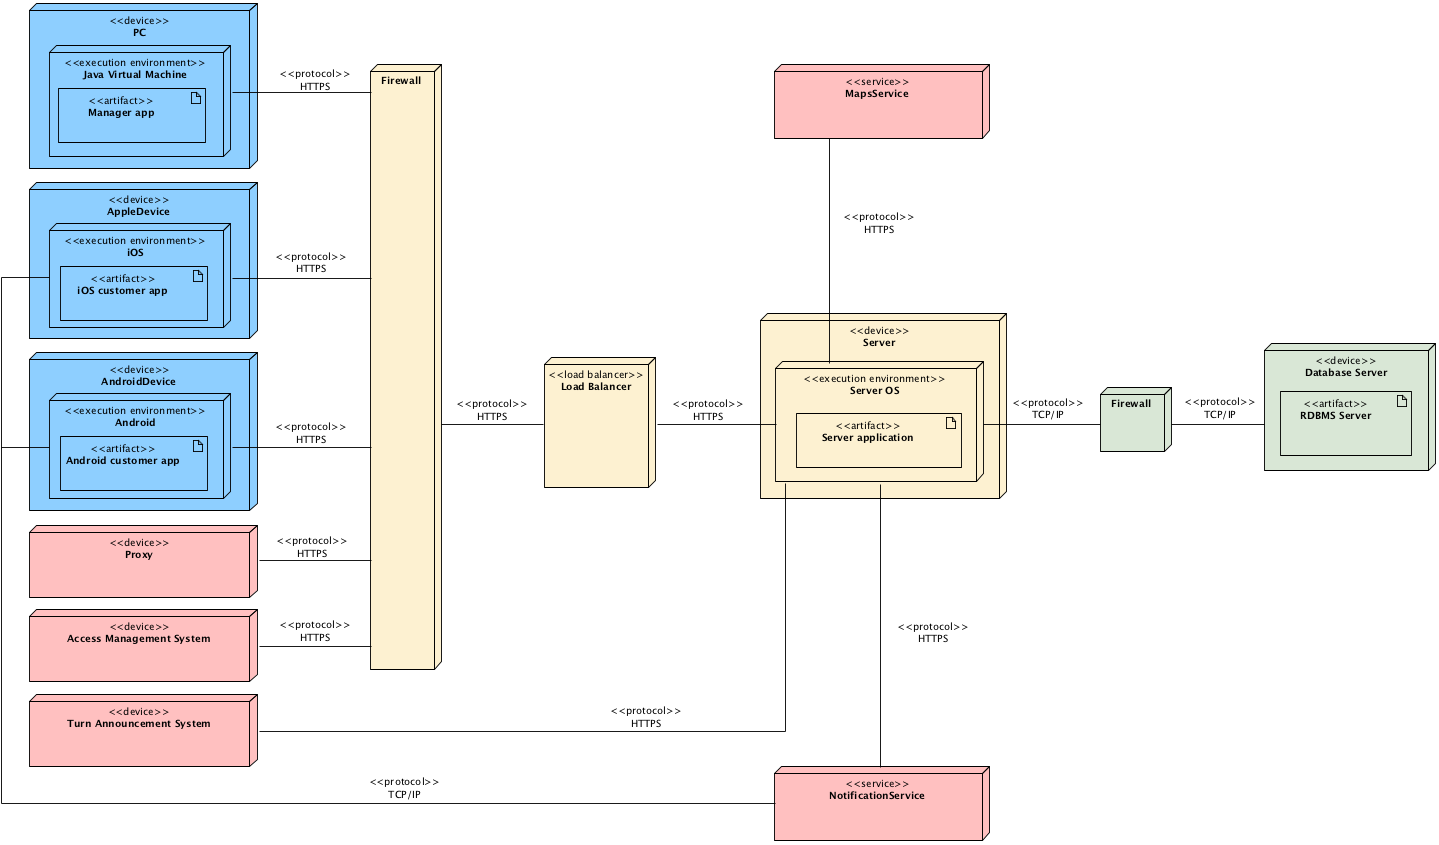
\includegraphics[width=\textwidth, height=\textheight, keepaspectratio]{pictures/deployment_diagram}
        \caption{Deployment diagram}
        \label{figure:deployment_diagram}
    \end{figure}
    Since CLup must be able to deal with all the customers requests (\hyperlink{NF1}{NF1}) and must be available the 99\% of the time (\hyperlink{NF5}{NF5}), the server can be replicated many times and a load balancer on the incoming requests allows the scalability of the server itself and spreads the workload between the replicas. \par
    In order to improve the security of the system (\hyperlink{NF6}{NF6}), a firewall has been added for requests incoming to the server and to the database. \par
    Since more than the 99\% of smartphones on the market run either iOS or Android\footnote{Mobile operating system market share worldwide: \par \url{https://gs.statcounter.com/os-market-share/mobile/worldwide}}, the development of the customer mobile application focuses on these two major operating systems. Hence, also considering the flexibility introduced by a RESTful API, the complexity of some CLup functions and the differences between the two platforms, two distinct mobile applications are going to be developed, each of them optimized for the mobile OS it is meant for. In this way, the mobile application (and the final user) benefits from all the advantages of native apps, including the possibility of caching and offline use. In particular, caching can be used to reduce the overall communication and to increase performance. \par
    Instead, since about 95\% of personal computers on the market run either Windows, macOS or Linux\footnote{Desktop operating system market share worldwide: \par  \url{https://gs.statcounter.com/os-market-share/desktop/worldwide}} and all of them are capable of running a Java Virtual Machine, a single Java application is suitable to provide store managers with an administrative tool that includes all the CLup functions destined to them.
    %%%%%%
    \section{Other design decisions}
    \label{section:design_decisions}
    By design, if a store is divided into product sections, its maximum occupancy is the sum of the ones of the product sections it is made by and can’t be manually modified by one of its managers. \newline\newline
    When a store closing time is reached, the queue of that store is emptied. \newline\newline
    When determining which customer can enter the store, the system allows entrances to each store trying to guarantee that each customer who placed a booking request for that store can start his visit to the store as soon as the specified desired time comes. \newline\newline
    A token is made by an unique identifier (UUID), which completely identifies the token itself, and a human-friendly identifier (HFID), which is the one readable by users and used locally by each store to identify the request it is associated with and announce it through the TAS. \newline\newline
    By design, the token UUID is provided to customers as a QR code. Thus, each proxy must be able to print QR codes and each AMS must be able to scan and read them. \newline\newline
    Each store has its own passepartout token, provided as a QR code, which is a special token used by store managers to manually regulate entrances and exits. \newline\newline
    All the interactions with and inside the system, with the exception of those passing through the ManagerInt, are not authenticated. When a manager logs in through the administrative tool, a unique authentication token is created on the server and returned to the administrative tool. Then, that token is used for HTTPS token-based authentication until it expires or until the manager logs out. Since there are no particular requirements concerning security, no constraints on further choices are introduced. \newline\newline
    When a manager changes the working hours, the maximum occupancy of a store (if it is not divided into product sections), the maximum occupancy of a product section or the safety threshold, even if the changes are applied when the store is closed, future booking requests may be affected by these changes. The same may also happen when deleting a product section. In fact, for example, a booking request might refer to a no more existing section or the store might not be open for the whole duration of the visit. In this case, those bookings are deleted and their customer informed through a push notification. \newline\newline
    Each app-customer is identified by a unique id, which is binded to the application itself. That id is also known as device token or appID, since it is a unique key for the app-device combination. Thus, no manual registration or login shall be implemented for app-customer. This design decision has been taken in order to develop a completely user friendly and easy to use mobile application. \newline\newline
    Each proxy is identified by a unique id, the proxyID, which is binded to the machine itself. \newline\newline
    Since the system shall recognize when a customer does not show up when it is his turn (i.e. when one of his visit requests is ready), it waits a certain amount of time before allowing another customer to enter the store. In other words, if that customer does not show up before the timeout, the related visit request is deleted and the customer must make another request in order to enter the store. By design, the timeout is of 2 minutes for booking requests and of 5 minutes for line-up requests. \newline\newline
    If a store is divided into product sections, customers can specify the ones they want to visit while making a new booking request. This allows the system to be aware of where they will be inside the store during their visit, and so, to better guarantee the absence of crowdings inside the stores. In fact, without that information, it is more difficult to try avoiding gatherings inside the product sections of the store. In terms of probability, the more the store approaches its maximum occupancy, the more that situation could be a threat to customers safety. For instance, it may happen that, even for a small amount of time, the current occupancy of a product section overcomes its maximum allowed value. CLup tries to avoid these unpleasant situations by managing accesses to the stores in two different modalities: in the first one, the given store is said to be in the ``green zone", while in the second one it is said to be in the ``yellow zone". The modality automatically changes whenever the store current occupancy is above a ``safety threshold", a parameter specified by the store manager. Details on the safety threshold and on the behaviour of the system in both modalities are provided in the relevant algorithms section. \newline\newline
    The system shall inform a customer when, according to his current position, should head towards the store. However, this information is based on an estimation of how long it takes for the customer’s turn to come. When that estimation exceeds the actual time needed, it happens that it is the customer’s turn but he is still on the way. To prevent people from gathering in front of stores waiting their turn, the timeout considered in the previous paragraph is extended by the difference between the estimated time of entrance known when sending the notification and the actual time in which the customer’s turn is announced. 
    
    \newpage
    \section{Runtime view}
    In all the following diagrams it is assumed that no cache is used on the customer mobile application and that the parameters included in the requests are valid. Furthermore, for the sake of readability of the diagrams, sometimes class parameters are not made explicit: ``classParameters" is just a placeholder for the attributes of the specified ``class" (with respect to the class diagram).
    \subsubsection{Customer opening the mobile app}
    This sequence diagram shows the flows of events and the interactions that happen when a customer opens the mobile application. If it is the app's first launch, the app-customer id is sent to the server, allowing for its (automatic) registration. Otherwise, all the active requests of that customer are retrieved. Finally, he specifies a city, obtaining all the chains and the autonomous stores located in that city. 
    \begin{figure}[H]
        \centering
        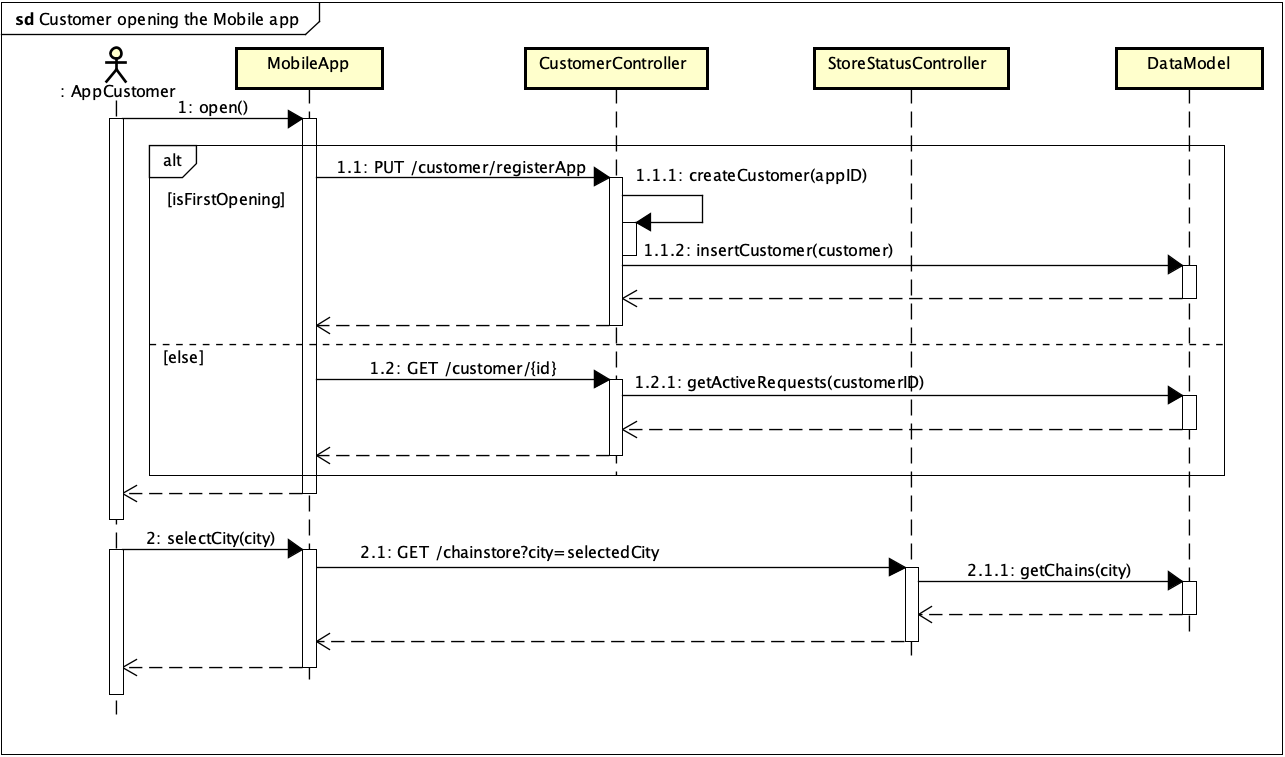
\includegraphics[width=\textwidth, height=\textheight, keepaspectratio]{pictures/sequence_diagrams/customer_opening_mobile_app}
        \caption{Customer opening the mobile app}
        \label{figure:customer_opening_mobile_app}
    \end{figure}
    \subsubsection{New booking request for a chain store}
    This sequence diagram shows the flows of events and the interactions that happen when an app-customer wants to book a visit to a store of a chain. He chooses the chain and the store, then forwards the request specifying all the parameters of a booking request. The request is placed only if there are no existing bookings of the same customer which overlap the new one in terms of specified time interval, if it starts after the queue disposal time of the store, if the store is open for the whole estimated duration of the visit and if all the people specified can actually enter the store according to the other bookings for the same time interval. \par
    If the request is not placed, alternative stores of the same chain and alternative time intervals for the same store are forwarded to the customer, who can choose one of them. Otherwise, the request is immediately placed. \par
    In this diagram it is assumed that the store is not filling up (i.e. no-app customer shall be notified of this event, according to the specific CLup functionality).
    \begin{figure}[H]
        \centering
        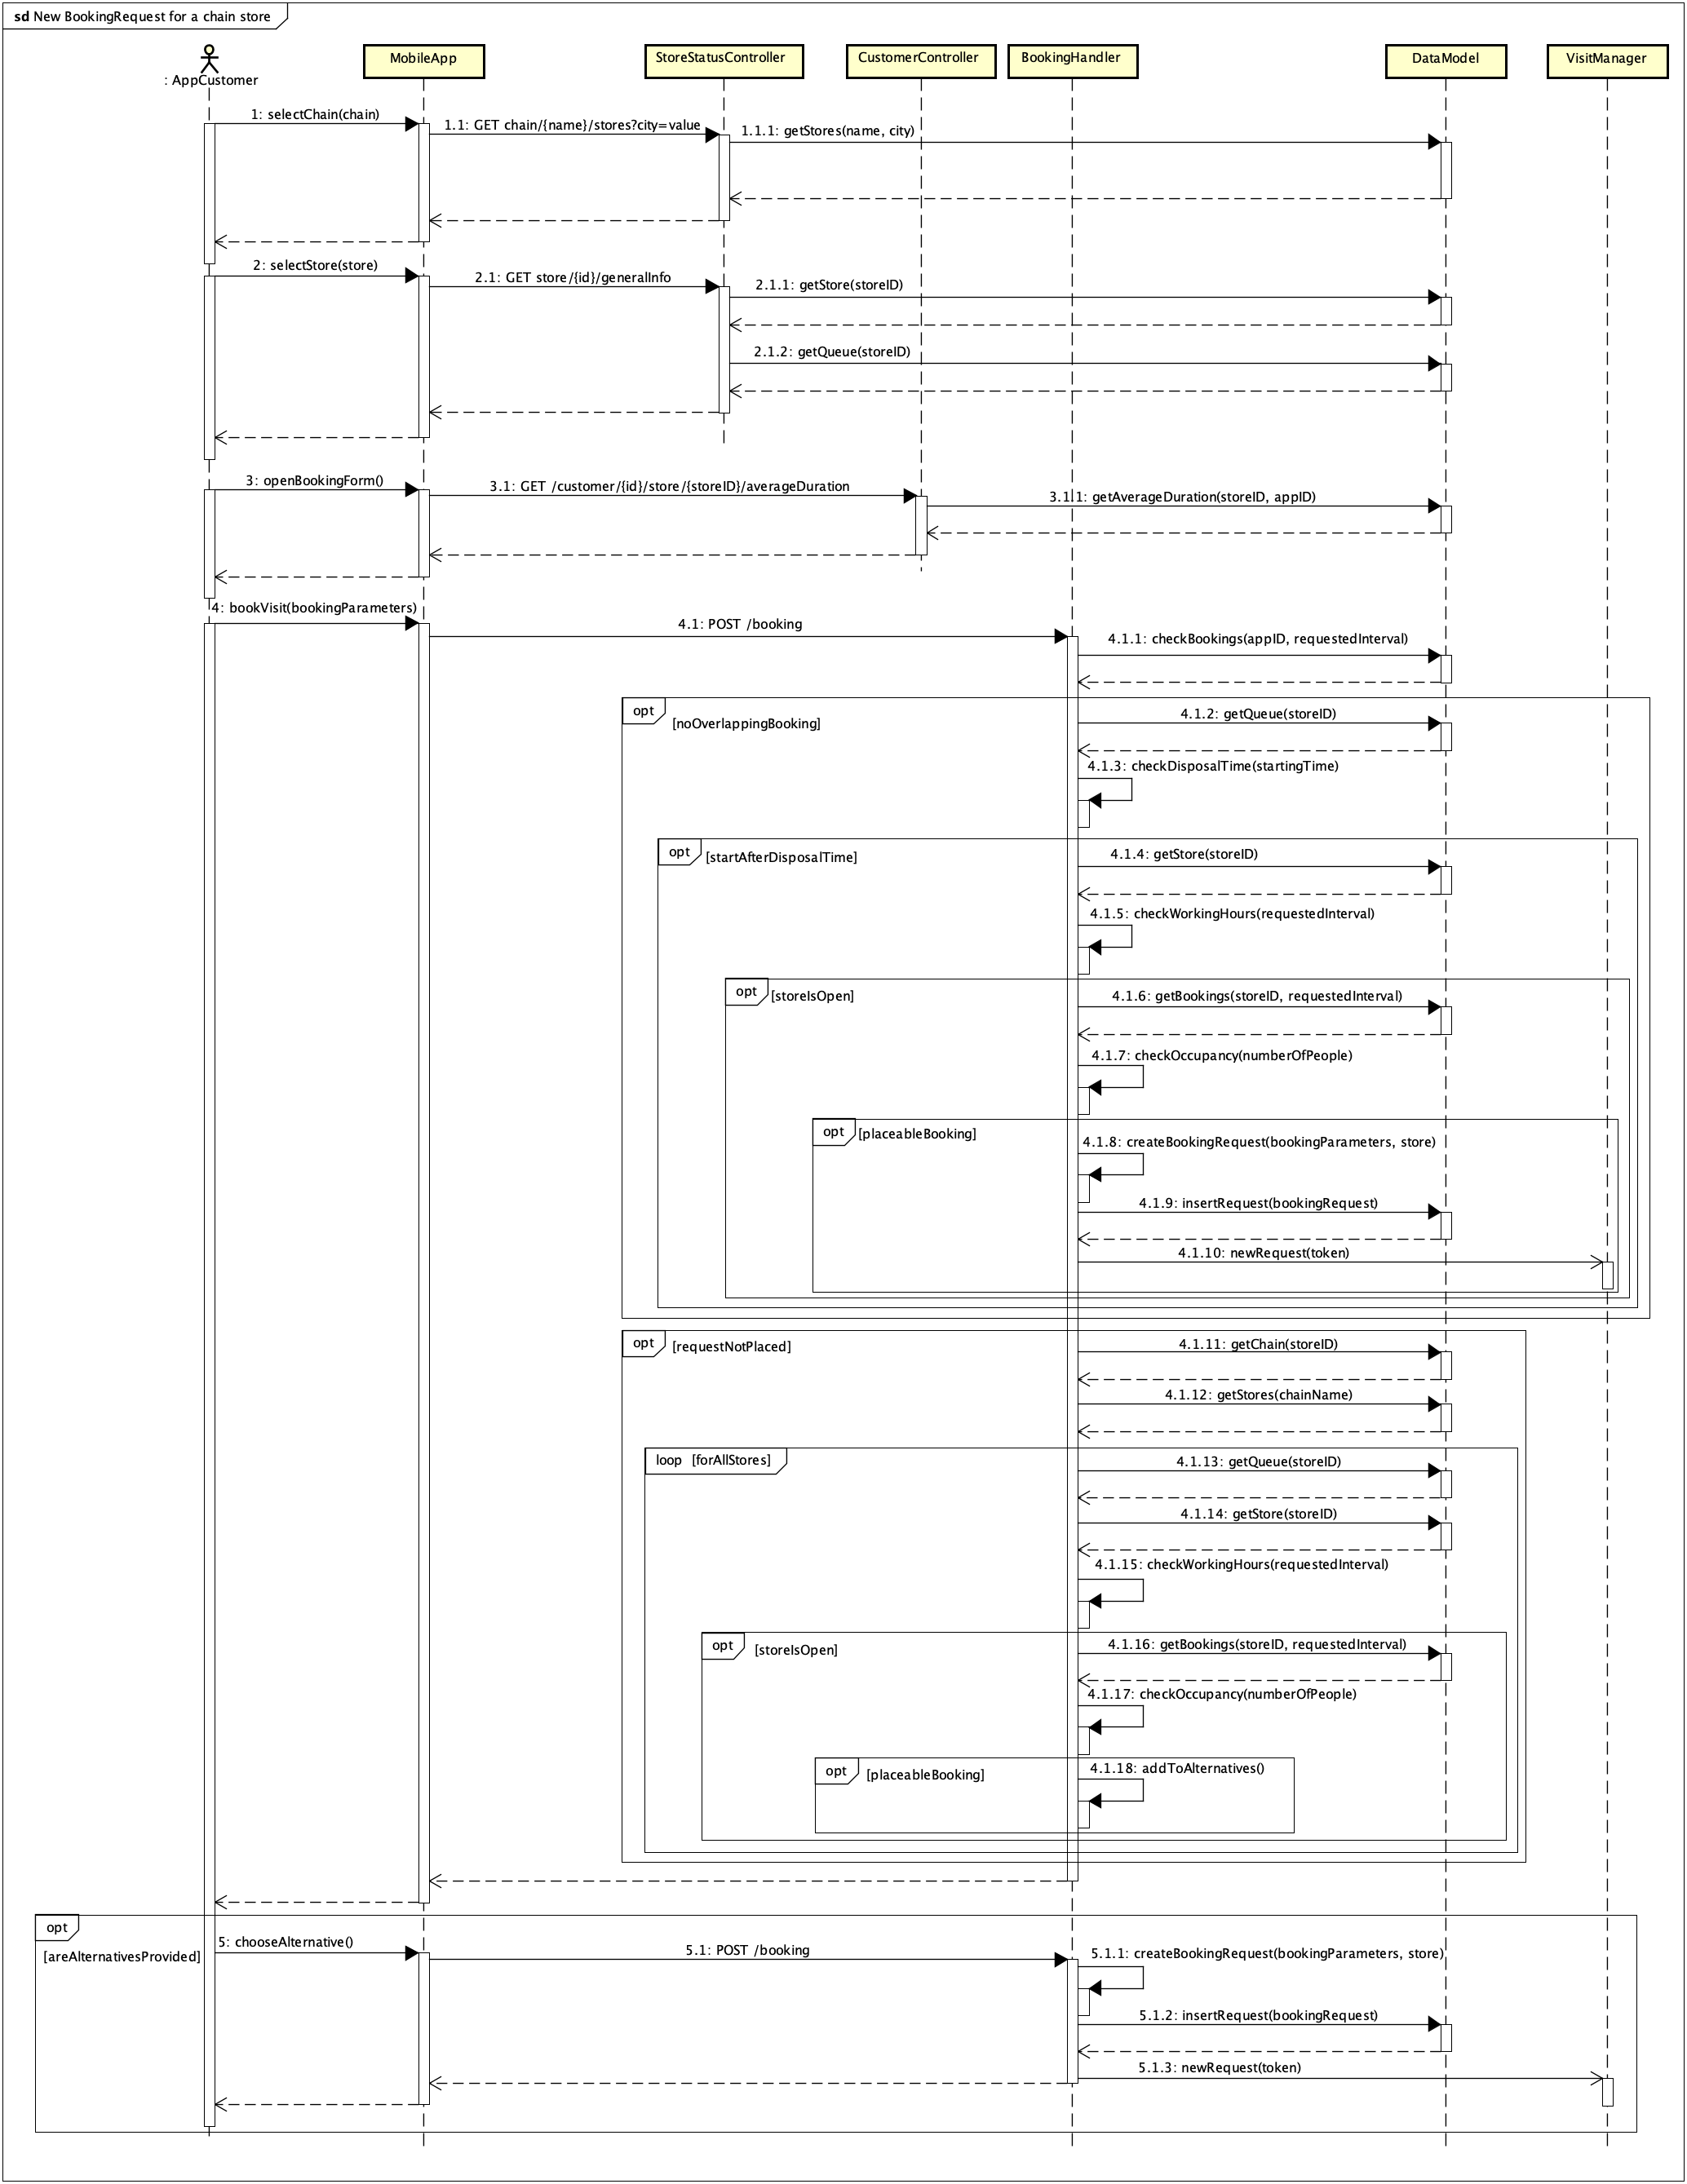
\includegraphics[width=.95\textwidth, height=\textheight, keepaspectratio]{pictures/sequence_diagrams/new_booking_request_for_a_chain_store}
        \caption{New BookingRequest for a chain store}
        \label{figure:new_bookingrequest_for_a_chain_store}
    \end{figure}
    \subsubsection{App line-up}
    This sequence diagram shows the flows of events and the interactions that happen when an app-customer wants to line-up for a store of a chain. He chooses the chain and the store. Then, he forwards the request specifying how many people are going to visit the store (including himself). If the store is open at that time and the customer is not in the queue of any other store, the request is placed. \par
    In this diagram it is assumed that the store is not filling up (i.e. no app-customer shall be notified of this event, according to the specific CLup functionality).
    \begin{figure}[H]
        \centering
        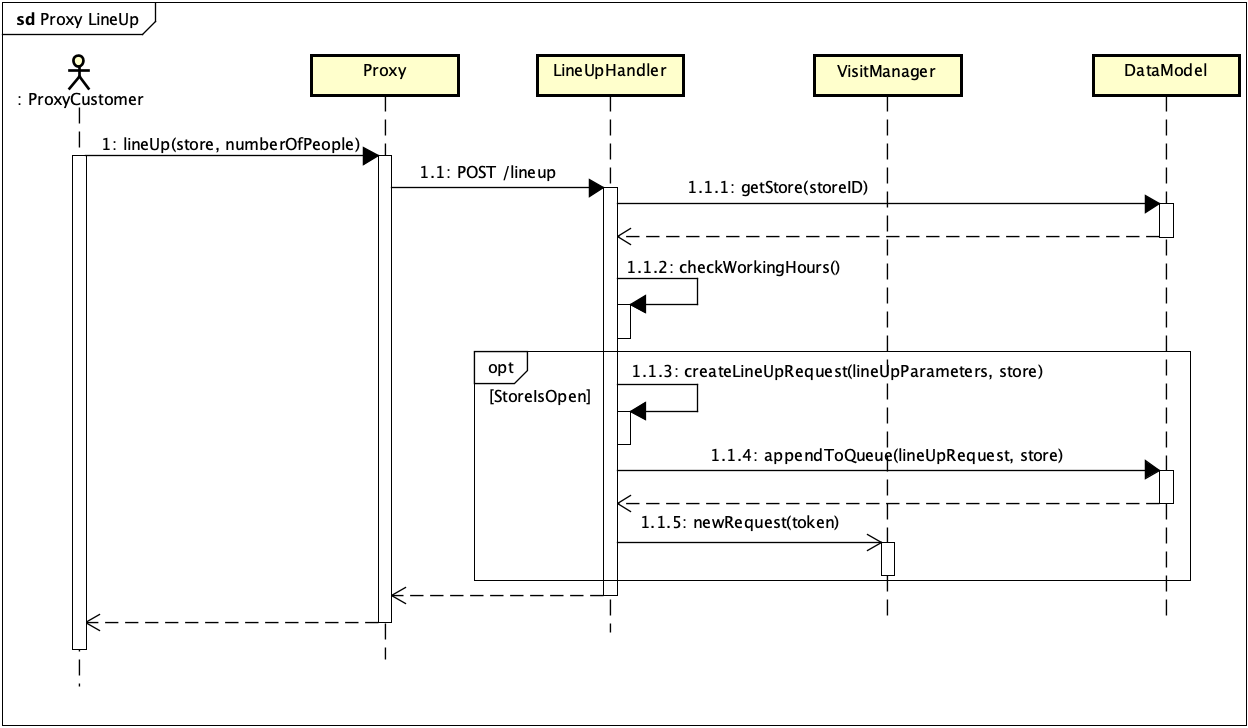
\includegraphics[width=\textwidth, height=\textheight, keepaspectratio]{pictures/sequence_diagrams/proxy_lineup}
        \caption{Line-up of an app-customer for a store}
        \label{figure:proxy_lineup}
    \end{figure}
    \newpage
    \subsubsection{Proxy line-up}
    This sequence diagram shows the flows of events and the interactions that happen when a proxy-customer wants to line-up for a store. The proxy forwards the request, which is accepted if the store is open. \par
    In this diagram it is assumed that the store is not filling up (i.e. no app-customer shall be notified of this event, according to the specific CLup functionality).
    \begin{figure}[H]
        \centering
        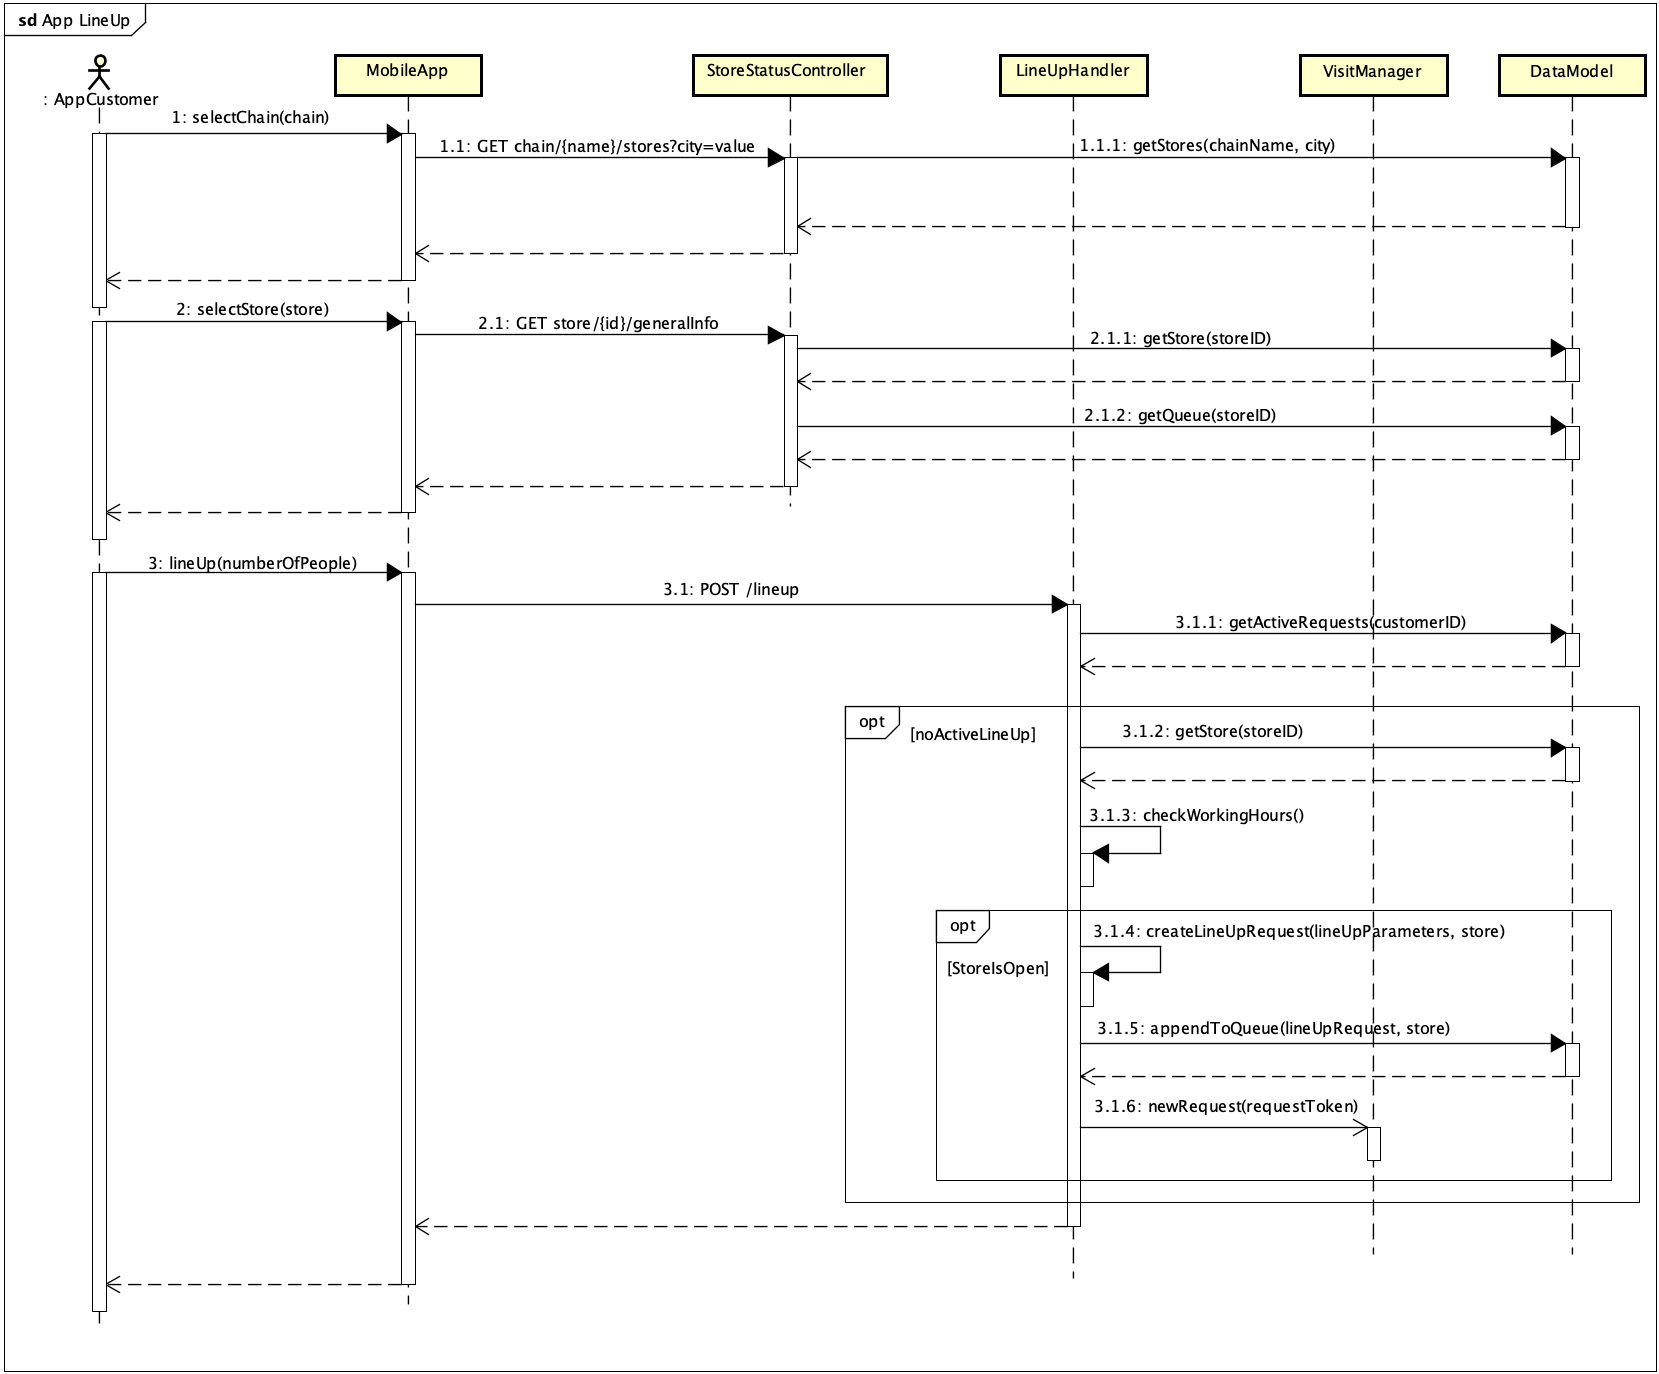
\includegraphics[width=\textwidth, height=\textheight, keepaspectratio]{pictures/sequence_diagrams/app_lineup}
        \caption{Line-up of a proxy-customer for a store}
        \label{figure:app_lineup}
    \end{figure}
    \newpage
    \subsubsection{A customer exits the store}
    This sequence diagram shows the flows of events and the interactions that happen when a customer exits a store and another one can enter it, if so. First, the request leaving the store is marked as completed. Then, the VisitManager, considering the actual status of the store, its queue and the its pending bookings, check who is the next one who can enter the store and marks his request as ready, announcing the turn via the TAS and, in the case of an app-customer, via a push notification.
    \begin{figure}[H]
        \centering
        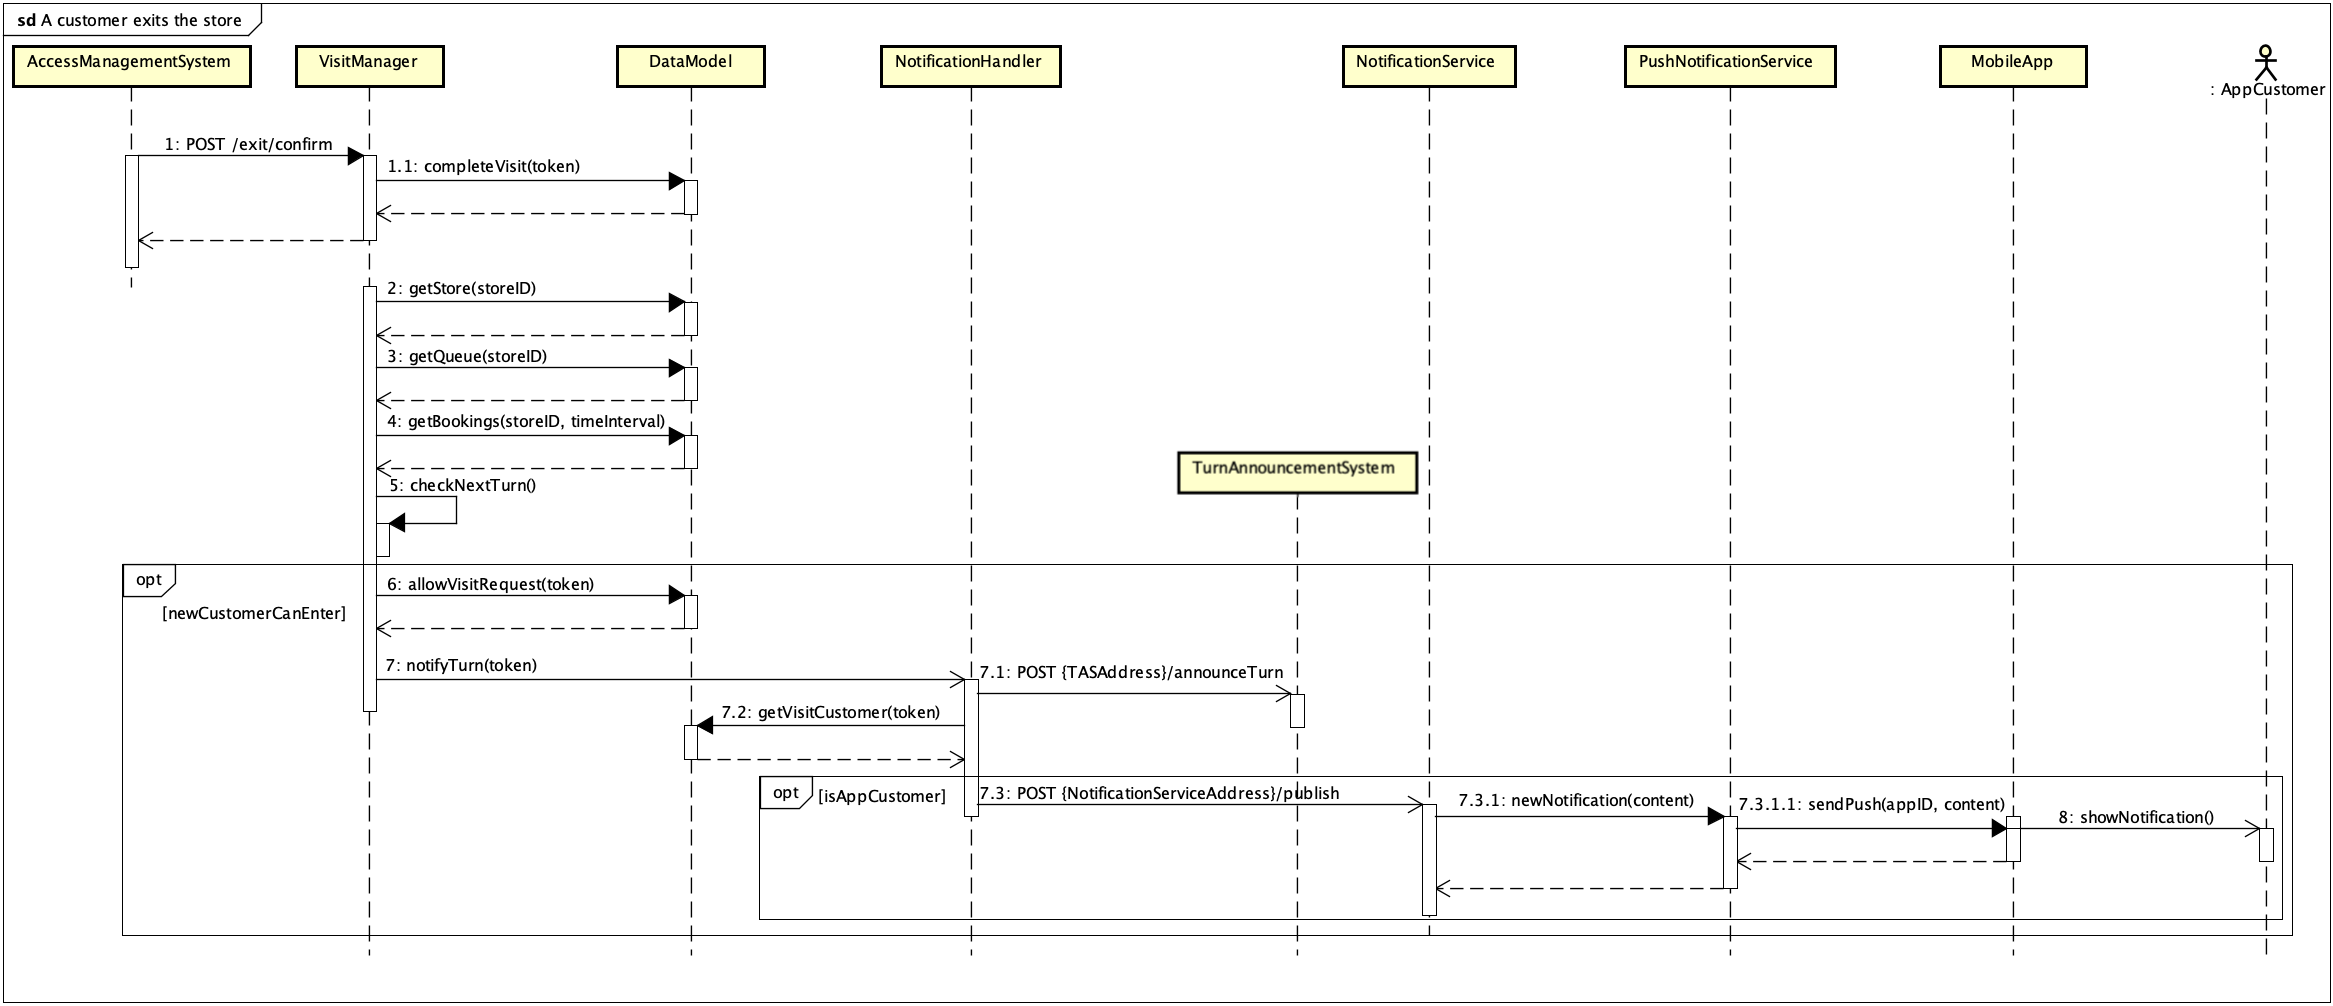
\includegraphics[width=\textwidth, height=\textheight, keepaspectratio]{pictures/sequence_diagrams/a_customer_exits_the_store}
        \caption{A customer exits the store}
        \label{figure:a_customer_exits_the_store}
    \end{figure}
    \newpage
    \subsubsection{Entering the store}
    This sequence diagram shows the flows of events and the interactions that happen when a customer wants to enter a store. He provides his visit token to the AMS, which forwards the access request to the server. If the request is ready, the access is granted and the AMS allows the customer to enter, counting the actual number of people entering the store (which can be only less or equal to the number specified in the request) and forwarding this information to the server. Finally, the visit can start and, if it was a line-up request, it is removed from the queue of the store. \par
    The sequence diagram showing the exit of a customer is analogous.
    \begin{figure}[H]
        \centering
        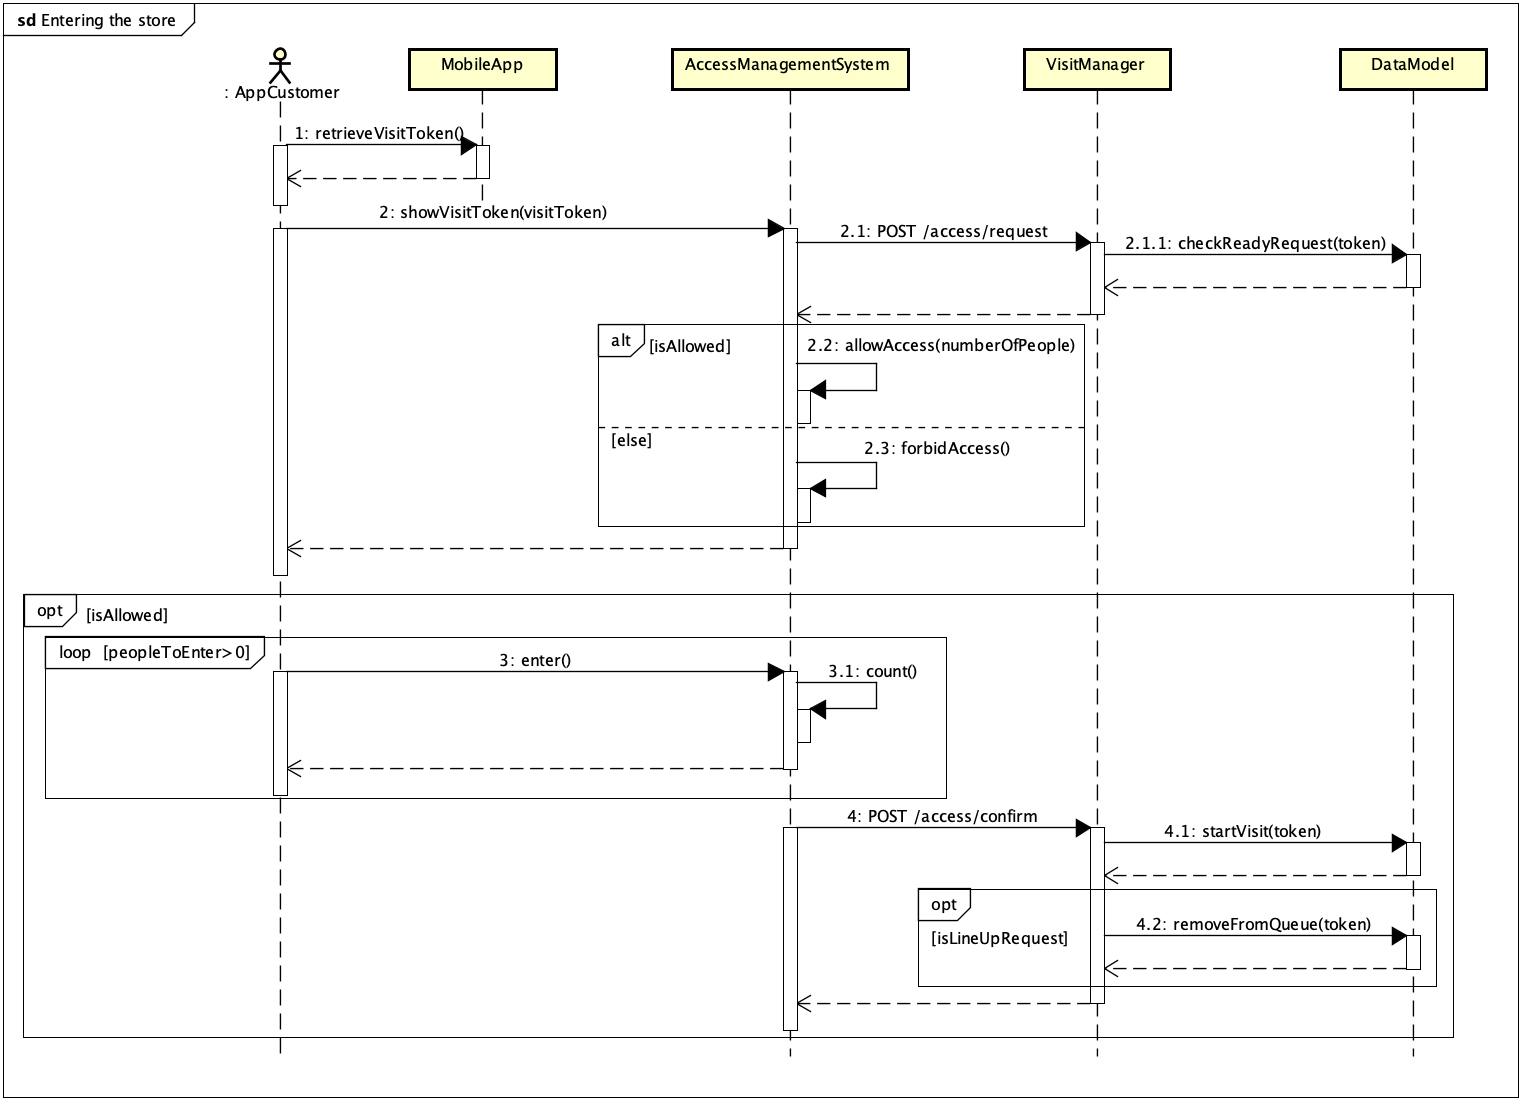
\includegraphics[width=\textwidth, height=\textheight, keepaspectratio]{pictures/sequence_diagrams/entering_the_store}
        \caption{Entering the store}
        \label{figure:entering_the_store}
    \end{figure}
    \newpage
    \subsubsection{Updating customer's position}
    This sequence diagram shows the flows of events and the interactions that happen when an app-customer automatically informs the system of his actual position. The system checks how long it would take for him to reach the store he lined-up for and, if he should start heading towards the store, the mobile application notifies him.
    \begin{figure}[H]
        \centering
        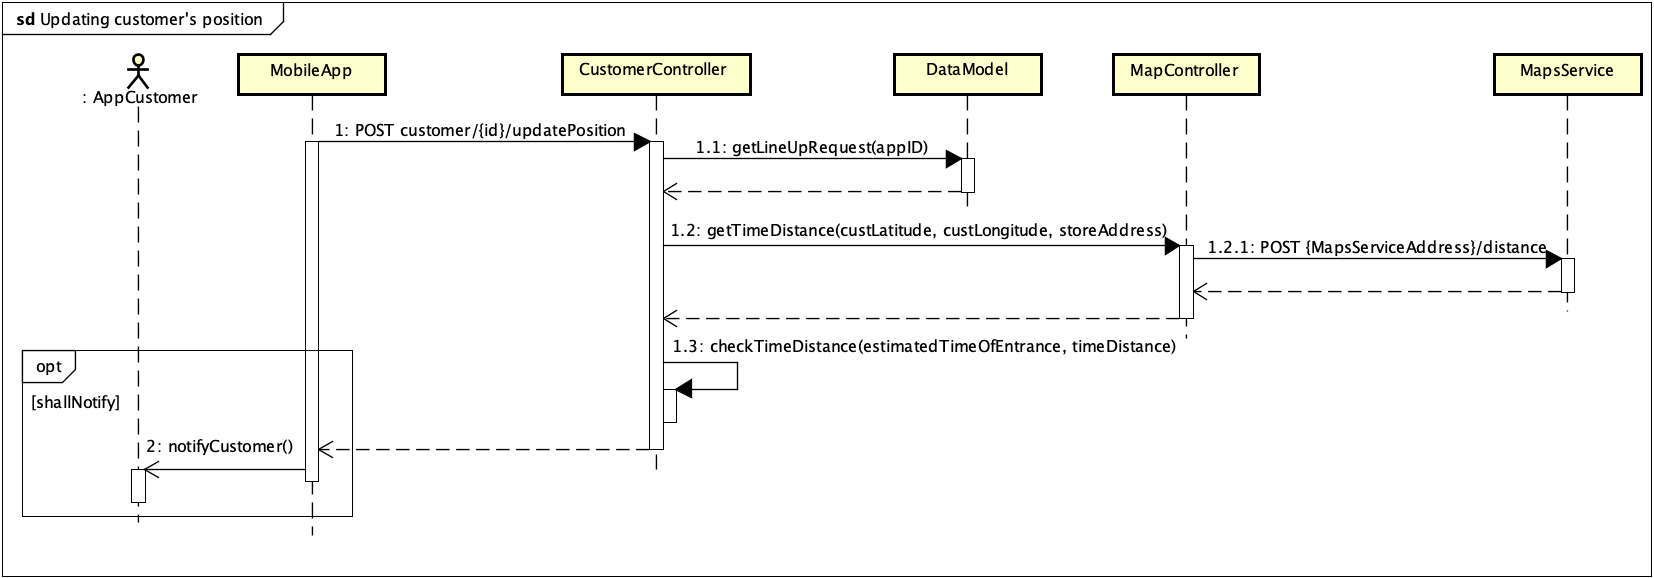
\includegraphics[width=\textwidth, height=\textheight, keepaspectratio]{pictures/sequence_diagrams/updating_customer_position}
        \caption{Updating the customer's position}
        \label{figure:updating_customer_position}
    \end{figure}
    \newpage
    \subsubsection{Manager opening the administrative tool}
    This sequence diagram shows the flows of events and the interactions that happen when a manager opens the administrative tool. He logs in, and, if the credentials are validated, he is provided with all the information about the stores he manages. When he finishes his job, he logs out.
    \begin{figure}[H]
        \centering
        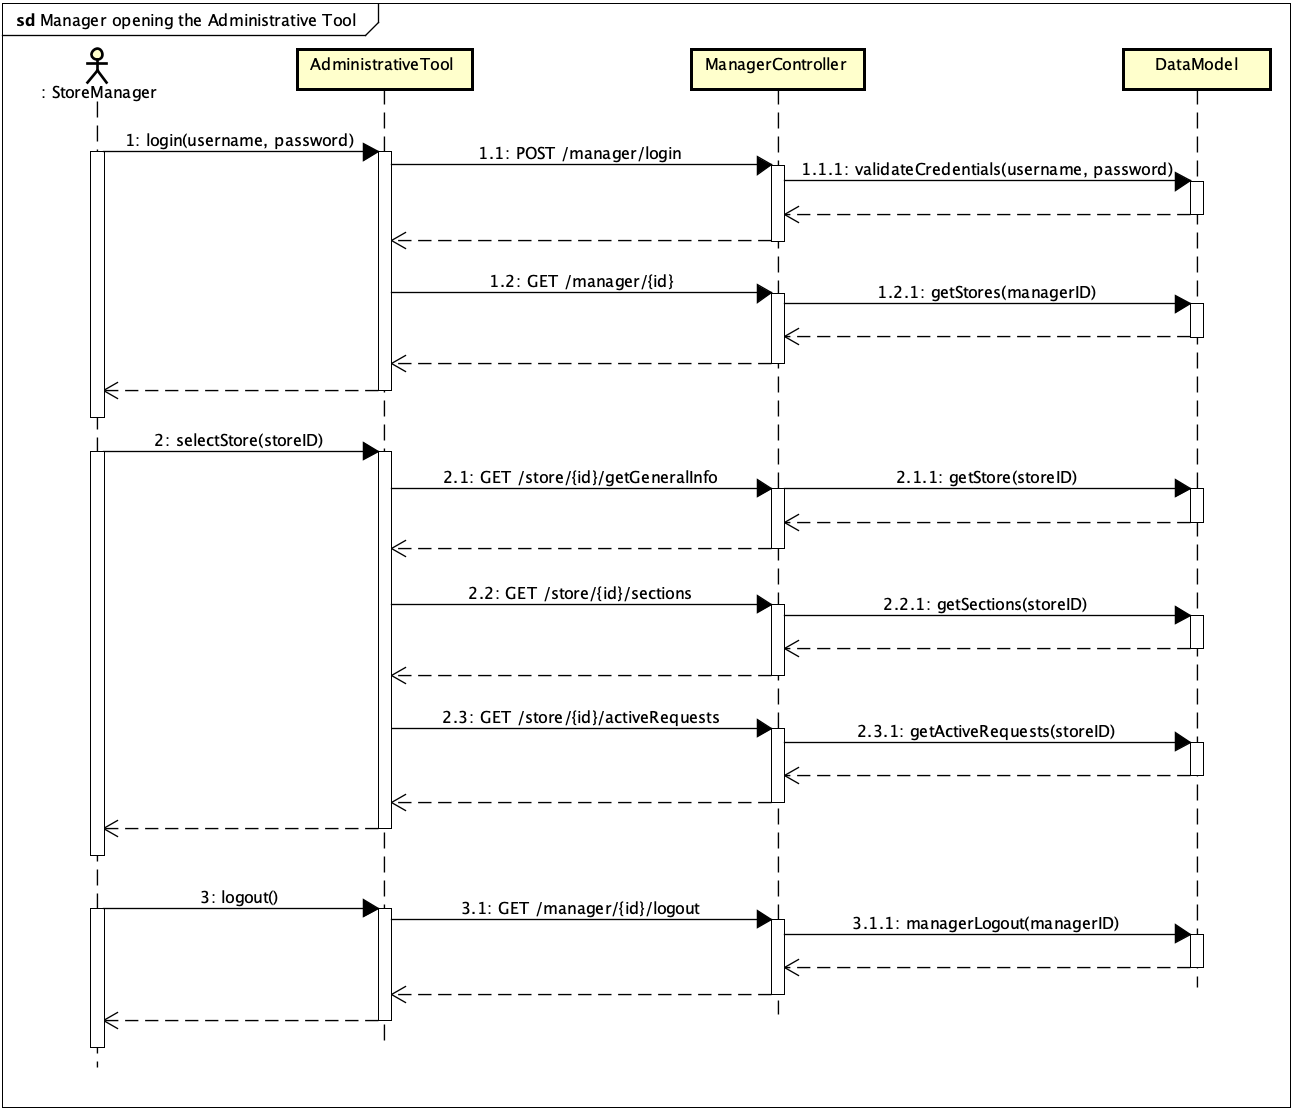
\includegraphics[width=\textwidth, height=\textheight, keepaspectratio]{pictures/sequence_diagrams/manager_opening_the_administrative_tool}
        \caption{Manger opening the administrative tool}
        \label{figure:manager_opening_the_administrative_tool}
    \end{figure}
    \newpage
    \subsubsection{Adding managers}
    This sequence diagram shows the flows of events and the interactions that happen when a manager wants to add another manager to one of the stores he manages (otherwise the operations is not allowed). If the manager he wants to add does not exist yet, a request of creation which includes the attributes of the new manager is forwarded to the server. If the manager he wants to add is an existing one, the new manager is added to the ones of the store.
    \begin{figure}[H]
        \centering
        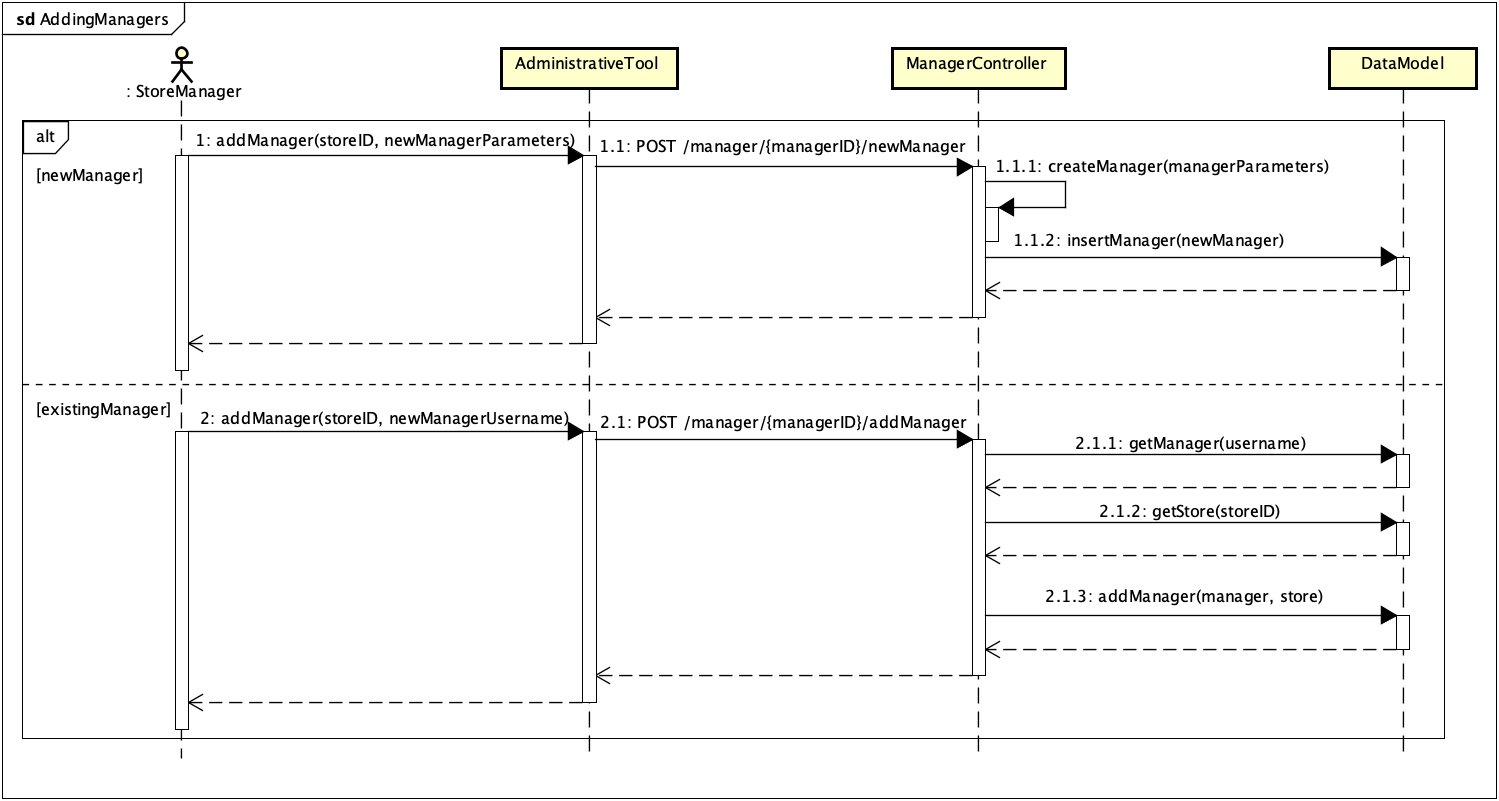
\includegraphics[width=\textwidth, height=\textheight, keepaspectratio]{pictures/sequence_diagrams/adding_managers}
        \caption{Adding managers}
        \label{figure:adding_managers}
    \end{figure}
    
    \newpage
    \section{Relevant algorithms}
    The following algorithm is the one designed for determining whether a customer who placed a visit request is allowed to enter the desired store. The algorithm is executed by the VisitManager and is described by means of pseudo-code instructions. Thus, it is not intended to provide constraints on how to actually implement it. \par
    The system handles accesses to a store in two different modalities, based on its current occupancy and \texttt{safetyThreshold} parameter. This last value can be specified by store managers only if the store is divided in product sections, and can assume an integer value between \texttt{0} and the \texttt{storeMaximumOccupancy - min\{productSectionMaximumOccupancy\}}. \par
    In the first modality, the current occupancy of the store is under or equal to its \texttt{safetyThreshold}, and so it is assumed to be highly safe. In this case, the store is said to be in the ``green zone". In the second modality, the current occupancy of the store is above its safetyThreshold and the system tries to avoid the potentially unpleasant situations described in section \ref{section:design_decisions}. In this case, the store is said to be in the ``yellow zone". \par
    The idea behind the algorithm is to differentiate the contribution that the number of people indicated in each visit requests has on the current occupancy of each product section, taking into consideration the kind of visit request and the zone in which the store actually is:
    \begin{itemize}
        \item The number of people for booking requests specifying product sections they intend to visit is always spread all over these sections. This is done taking into consideration, for each specified section, their maximum occupancies. Indeed, their current occupancies are incremented (or decremented, when exiting) by a value equal to the number of people willing to visit them, scaled on the ratio between each section’s maximum occupancy and their sum. In fact, it is reasonable to say that a customer, over the entire visit, will be in each product section only for a partial amount of the visit duration, that is, on average, related to the dimension of that section with respect to the other selected ones, represented by their maximum occupancy. 
        \item The number of people for line-up requests and for all other booking requests is considered in two different ways, taking into consideration the zone in which the store belongs to:
        \begin{itemize}
            \item In the green zone, the store is considered sufficiently empty, hence highly safe. For this reason, whenever customers who made line-up requests or booking requests without specifying product sections enter or exit the store, the only affected parameter is the store’s current occupancy: product sections’ current occupancies are not incremented (or decremented, when exiting).
            \item In the yellow zone, the store is filling up. For this reason,  whenever customers who made line-up requests or booking requests without specifying product sections enter or exit the store, their contribution (increment or decrement) to each product section is equal to the number of people specified in the request. However, in order to correctly decrement product sections’ current occupancies when these customers exit the store, it is necessary to know how many of these kinds of customers (but not whom) entered the store while in the yellow zone. In the algorithm, this information is represented by the ``\texttt{yellowEntrances}" variable, which gets initialized to \texttt{0} whenever a store enters the yellow zone.
        \end{itemize}
    \end{itemize}
    In all of the previous cases, the current occupancy of the store is always incremented (or decremented) by the actual number of people entering (or exiting), without considering how the different current occupancies of the store’s product sections are incremented (or decremented). \par
    Moreover, when more than one person associated with the same visit request enters the store, the system must cope with the case in which the safetyThreshold is immediately crossed: to do so, the algorithm ``splits" the contribution that the number of people associated with the visit request has on all the store occupancies. In fact, each person associated with the request is treated according to the rules of the green zone until the threshold is not reached. When the threshold is crossed, the remaining people are treated according to the rules of the yellow zone. \par
    Applying this algorithm when deciding whether a visit request can or cannot enter the store leads to the desired behaviour: in the yellow zone, only booking requests specifying product sections can maximize the store occupancy while guaranteeing a high degree of safety inside the shop. The maximum number of people that can actually be in the store at the same time is dynamically determined by the status of the product sections. \par 
    Indeed, the number of people inside the store is maximized only by specific combinations of booking requests on the different product sections. \par
    However, this can be only done if the store is divided into product sections: otherwise, accesses are managed only taking into consideration the store’s current and maximum occupancy. \newpage
    Given a visit request ``\texttt{toAllow}", it performs the following operations:
    \begin{lstlisting}[language=pseudocodeDD]
Store toVisit = toAllow.selectedStore
/* Execute following code block if the customers can enter  
   the store without exceeding its maximum occupancy
*/
if (toVisit.currentOccupancy + toAllow.numberOfPeople <= 
  toVisit.maximumOccupancy) {
  /* If the customer did a line-up or a booking for a store 
     not divided in product sections, then the request is 
     obviously accepted
  */
  if (toVisit has not product sections)
    toAllow.allowVisitRequest()
  /* If the store is divided in product sections, then the 
     request must be correctly analyzed
  */
  else {
    /* If the store will be in yellow zone accepting the 
       visit request:
    */
    if (toVisit.currentOccupancy + toAllow.numberOfPeople > 
      toVisit.safetyThreshold) {
      /* over is a variable which value equals to the number 
         of customers of the requests that exceed the green 
         zone
      */
      int over = min(toVisit.currentOccupancy + 
        toAllow.numberOfPeople - toVisit.safetyThreshold, 
        toAllow.numberOfPeople)
      /* under is a variable which value equals to the number
         of customers of the request that the store can  
         accept before entering the yellow zone
      */
      int under = toAllow.numberOfPeople - over
      /* If the customers did a line-up or did not specify 
         the desired product sections while making the 
         booking request, 'over' is the value that is added 
         to the occupancy of each product section.
         In case there exist a product section which would 
         exceed its maximum occupancy, the request cannot be 
         allowed
      */
      if (toAllow is LineUpRequest or (toAllow is 
        BookingRequest and 
        toAllow.specifiedProductSections is empty)) {
        foreach (productSection in toVisit.productSections)
          assert productSection.currentOccupancy + over <= 
            productSection.maximumOccupancy else {return}
            toAllow.allowVisitRequest()
        }
      /* If, instead, the customers specified some product 
         sections their occupancy is incremented by 'over' 
         scaled down, as previously specified. In case there 
         exist a product section which would exceed its 
         maximum occupancy, the request cannot be allowed
      */
      else{ 
        int sumOfMaxOccupancies = 0
        foreach (productSection in toVisit.productSections)
          sumOfMaxOccupancies +=   
            productSection.maximumOccupancy
        foreach (productSection in toVisit.productSections)
          assert productSection.currentOccupancy + 
            toAllow.numberOfPeople * 
            productSection.maximumOccupancy / 
            toVisit.sumOfMaxOccupancies <= 
            productSection.maximumOccupancy 
          else {return}
        toAllow.allowVisitRequest()
      }
    }
    /* If, by allowing customer to enter the store, it would 
       not get in yellow zone, the visit request is accepted
    */
    else
      toAllow.allowVisitRequest()
    }
}
    \end{lstlisting}
    \newpage
    When a customer begins a visit to the store, the following algorithm must be executed by the VisitManager. The visit request is referred to as  ``\texttt{entering}".
    \begin{lstlisting}[language=pseudocodeDD]
Store toVisit = entering.selectedStore
/* Execute following code block if the store is not divide
   in product sections or if the customers didn't specified
   product sections while creating the booking or if the 
   customers did a line-up
*/
if(entering is LineUpRequest or 
  (entering is BookingRequest and
  entering.specifiedProductSections is empty)) {
  int over = toVisit.currentOccupancy +   
    entering.numberOfPeople - toVisit.safetyThreshold
  if (over > 0) { 
    /* yellowEntrances counts how many customers entered 
       the store in yellow zone without specifying the 
       desired product sections
    */
    toVisit.yellowEntrances += over
    foreach (productSection in toVisit.productSections)
      productSection.currentOccupancy += over
    }
}
/* Execute following code block if the customers booked a 
   visit and specified some product sections
*/
else {
  int sumOfMaxOccupancies = 0
  foreach (productSection in toVisit.productSections)
    sumOfMaxOccupancies += 
    productSection.maximumOccupancy
  /* The specified product sections' current occupancies 
     is updated
  */
  foreach (productSection in toVisit.productSections)
    productSection.currentOccupancy += 
      entering.numberOfPeople *          
      productSection.maximumOccupancy / sumOfMaxOccupancies
}
// Then, the store's current occupancy is updated
toVisit.currentOccupancy += entering.numberOfPeople
    \end{lstlisting}
    \newpage 
    When a customer ends a visit to the store, the following algorithm must be executed by the VisitManager. The visit request is referred to as  ``\texttt{exiting}". 
    
    \begin{lstlisting}[language=pseudocodeDD]
Store toVisit = exiting.selectedStore
/* Execute following code block if the store is in yellow 
   zone and the customers exiting did a line-up or didn't 
   specified product sections when booking
*/
if (toVisit.currentOccupancy > toVisit.safetyThreshold and 
  (exiting is LineUpRequest or (
  exiting is BookingRequest and 
  exiting.specifiedProductSections is empty)) {
  /* Execute following code block if since the store is in 
     yellow zone some customers which information about 
     desired product sections entered the store
  */
  if (toVisit.yellowEntrances > 0) {
    /* The following variable's value will be equal to the 
       number of the customers that the variable 
       yellowEntrances must be decremented for
    */
    int yellowToConsider
    /* In this case, yellowEntrances must be decremented 
       for a lower value than the number of the customers 
       exiting the store
    */
    if (toVisit.currentOccupancy - 
      toVisit.safetyThreshold < 
      exiting.numberOfPeople)
      yellowToConsider = toVisit.safetyThreshold - 
      toVisit.currentOccupancy
      /* In this other case, yellowEntrances must be 
         decremented by the number of customers exiting
      */
    else 
      yellowToConsider = exiting.numberOfPeople
    /* We must also update the current occupancy of all the
       stores' product sections since they were altered
    */
    foreach (productSection in toVisit.productSections)
      productSection.currentOccupancy -=
        min(toVisit.yellowEntrances, yellowToConsider)
    toVisit.yellowEntrances -= 
      min(toVisit.yellowEntrances, yellowToConsider) 
    }
}




/* Execute following code block if the store is in green 
   zone or the customer exiting specified product sections 
   while booking
*/
else {
  int sumOfMaxOccupancies = 0
  foreach (productSection in toVisit.productSections)
    sumOfMaxOccupancies += productSection.maximumOccupancy
  foreach (productSection in toVisit.productSections)
    productSection.currentOccupancy -= 
      entering.numberOfPeople * 
      productSection.maximumOccupancy / 
      sumOfMaxOccupancies
}
// Then, the store's current occupancy is updated
toVisit.currentOccupancy -= exiting.numberOfPeople
\end{lstlisting}
    Whenever a visit ends, the VisitManager retrieves all the pending visit requests for the same store and determines the new visit requests to allow, taking into consideration their time of creation (in case of line-ups) or their desired starting time (in case of bookings).
    \newpage
    \subsection{Algorithm for handling with visit token loss}
    Whenever a customer inside the store is not able to retrieve his visit token, he is supposed to interact with the store manager, that will allow him to exit the store with the store’s passepartout. However, when the customer exits the store, CLup cannot trace back his actual visit request. Thus, this could lead to a situation in which a visit request remains forever in the active state. Moreover, for safety and consistency reasons, the system cannot update the store and product sections’ current occupancies, since there is no information about the kind of visit request associated with the interested customers. \par
    For this reason, an algorithm to cope with this kind of situation is required. This algorithm, executed by the VisitManager, takes a ``snapshot" of the visits in progress whenever a group of people, within a reasonably short amount of time, exits the store thanks to the passepartout, also keeping track of their actual number. From that moment on, whenever a visit included in the snapshot correctly ends, the algorithm removes it from the snapshot. If the sum of the number of people in the visit in progress which are left in the snapshot is equal to the ones who used the passepartout, then the system can be sure that these are the visits that can be safely and correctly ended. Only at this point, the occupancy of the store can be updated. \par
    The algorithm should also guarantee that it correctly ends even when other customers exit thanks to the passepartout while it is already running. To accomplish that, it should perform a union between the set of in progress visits of the already running execution and the new set of in progress visits in the store, and sum the amount of people exiting the store thanks to the passepartout with the one of the already running execution.

    \subsection{Algorithm for providing the estimated time of entrance}
    In order to avoid unpleasant situations in which physical queues arise due to customers arriving to the store before their turn is announced, the Visit Manager should run an algorithm that calculates a reasonably precise estimation of the time each customer has to wait before accessing the store he lined-up for. \par
    To do so, whenever a visit in a given store is completed,  a customer cancels his pending or ready request for that store, or a new line-up request is placed, the algorithm should run for all the pending line-up requests of that store that are affected by that event. For each of them, the algorithm should take into account all the visit requests supposed to be ready before it (i.e. previously made line-up requests and booking requests with starting time less then or equal to the estimated starting time of the current line-up request), considering the approximate start and duration of their visit. Thus, to correctly perform the estimation, it is necessary that the average duration of a visit to each store is reasonably precise. 
    
\chapter{User interface design}
    \section{Mobile application user interface}
    \begin{multicols}{2}
        \begin{figure}[H]
            \centering
            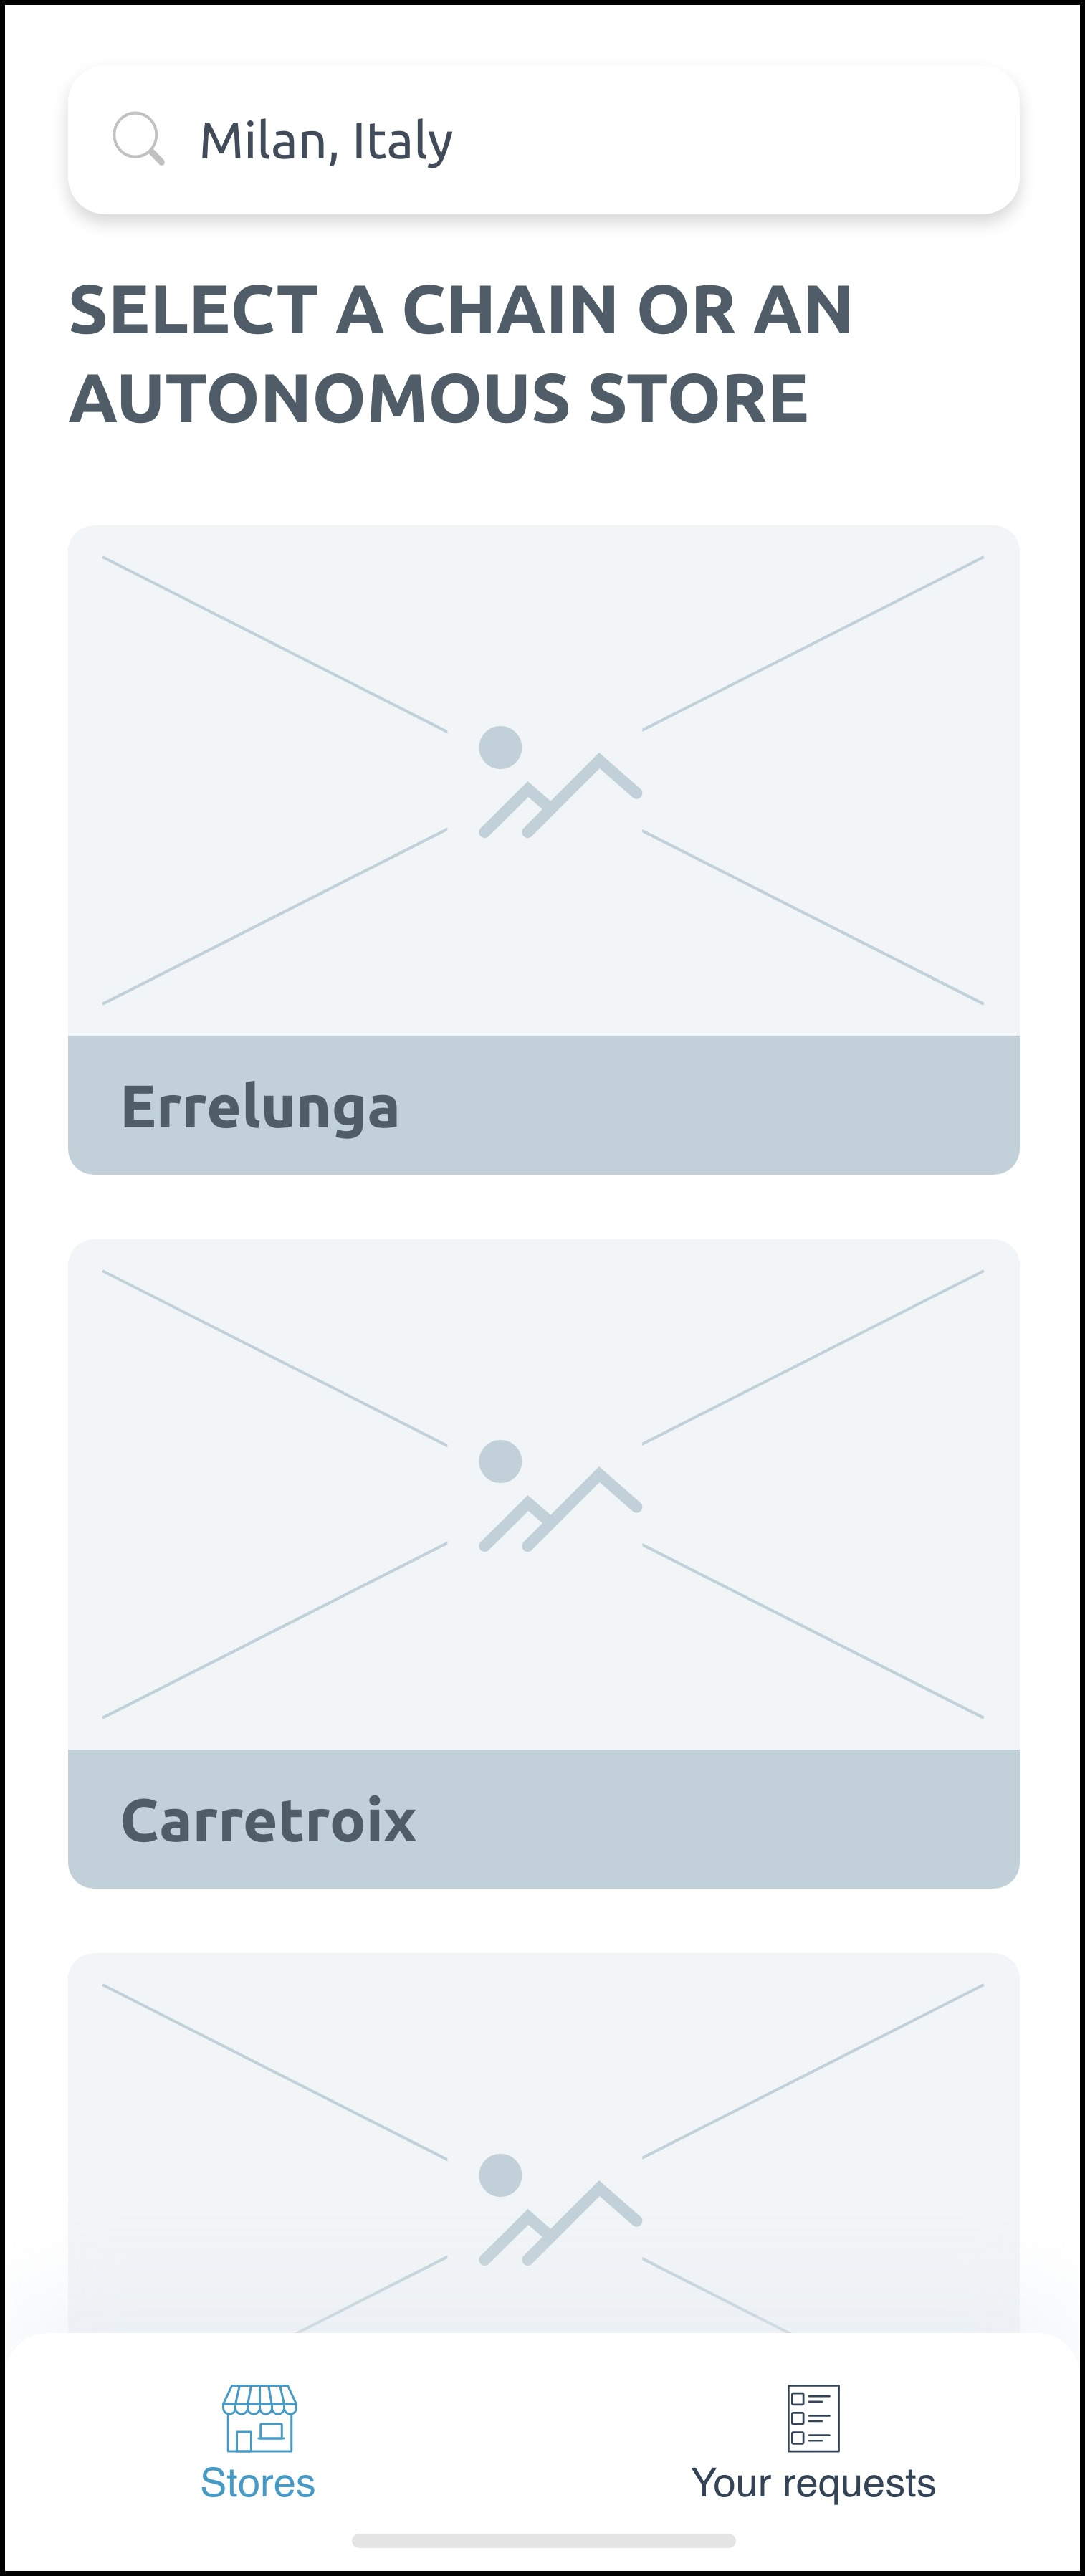
\includegraphics[width=\textwidth, height=.55\textheight, keepaspectratio]{pictures/mockups/select_chain}
            \captiondd{Mockup 1 -- Select a chain or an autonomous store}{Mockup showing the list of chains and stores located in a certain city (Milan). It is from the first tab of the GUI}
            \label{figure:mockup_1}
        \end{figure}
        \begin{figure}[H]
            \centering
            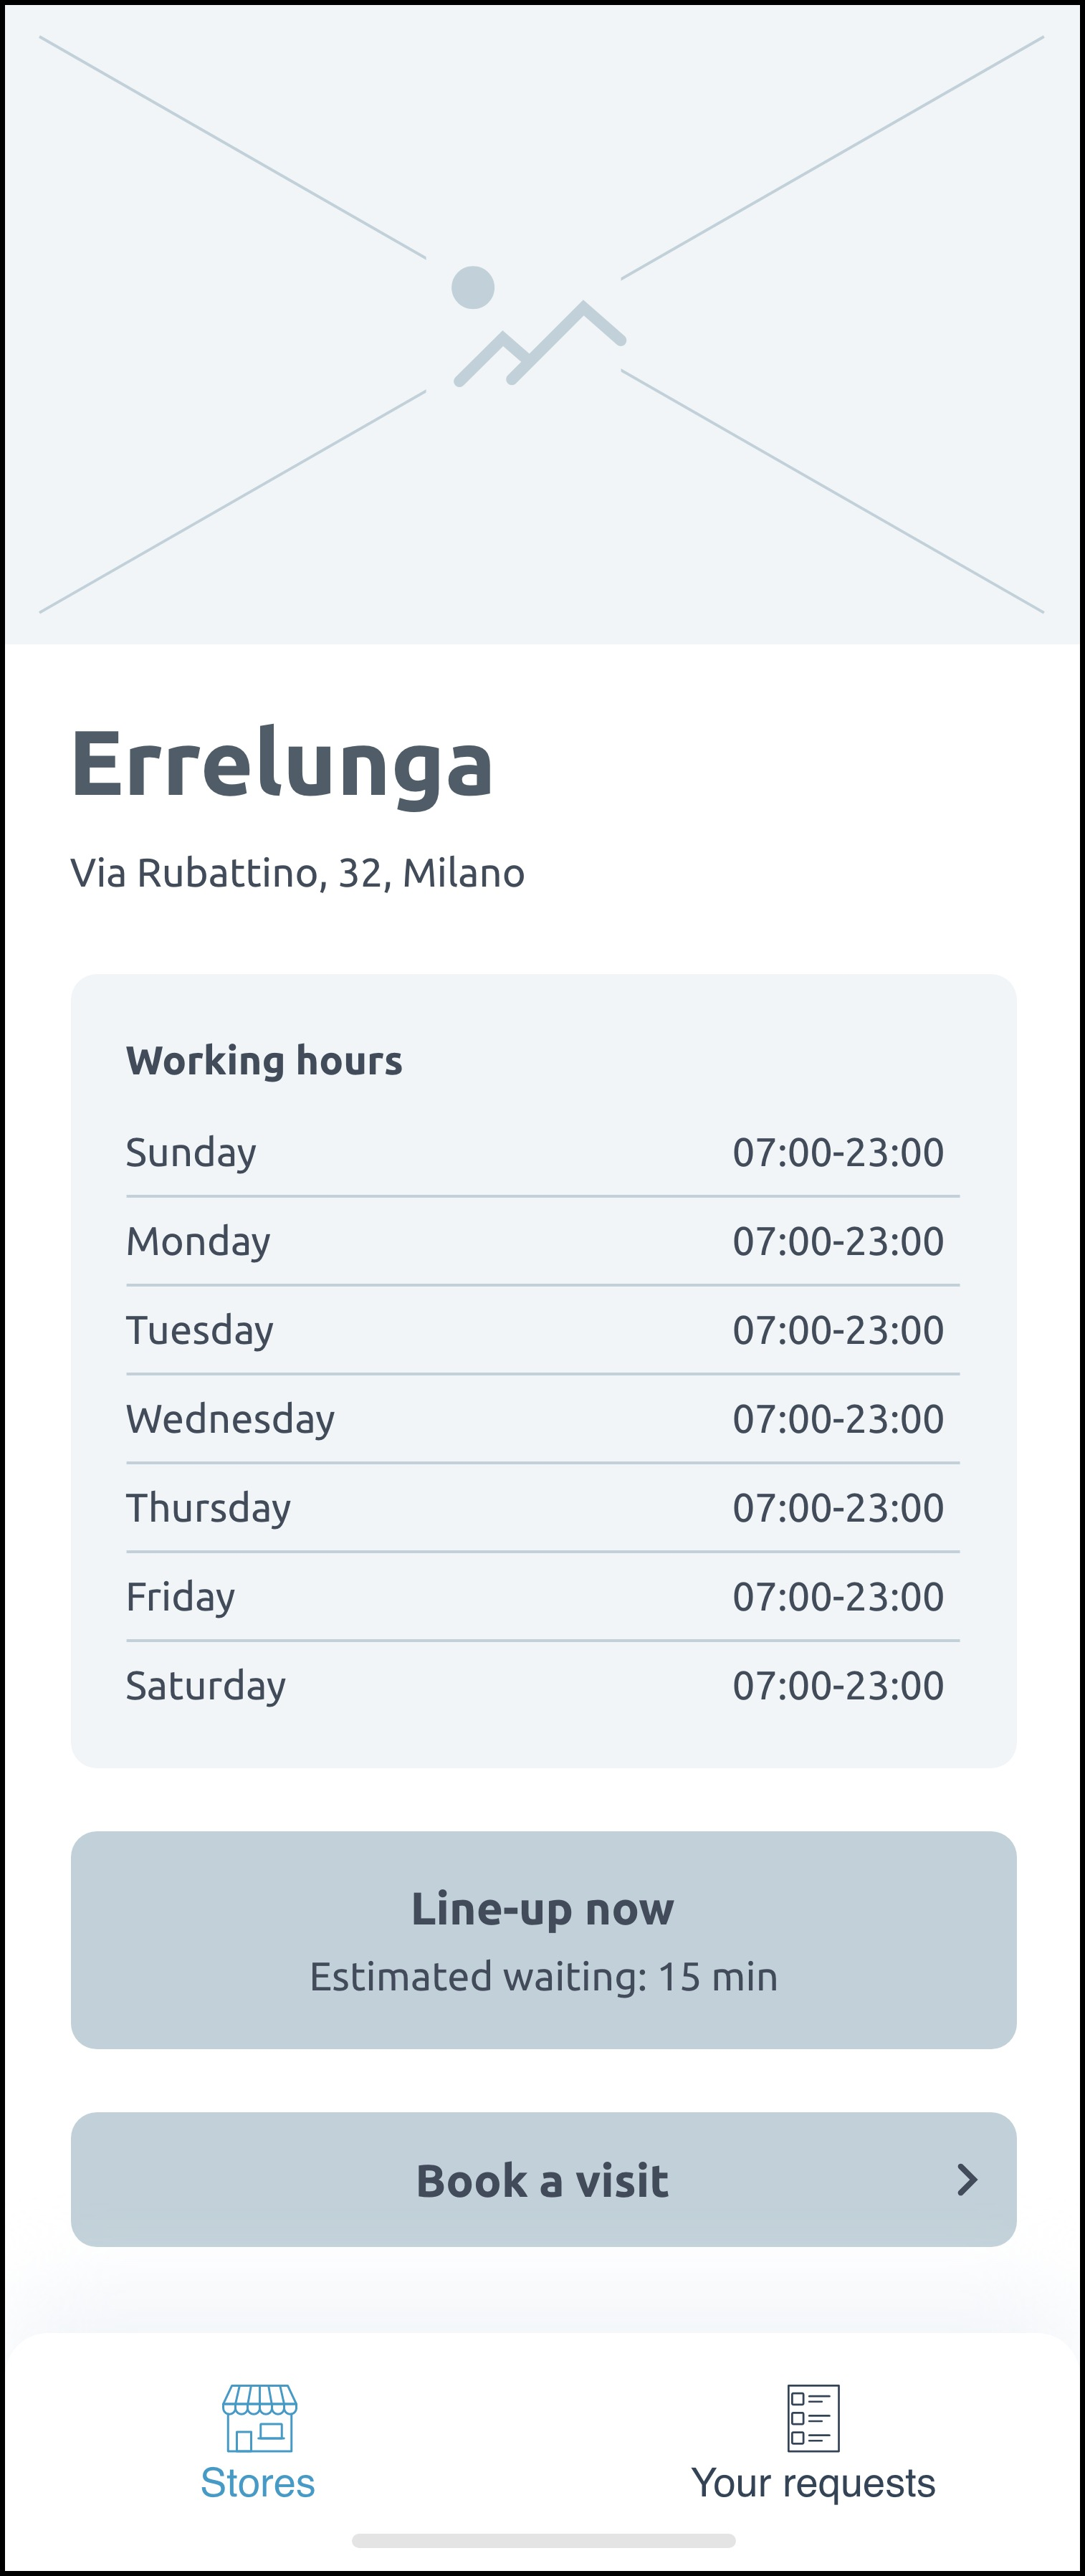
\includegraphics[width=\textwidth, height=.55\textheight, keepaspectratio]{pictures/mockups/store_view}
            \captiondd{Mockup 2 -- Store details}{Mockup showing the details of a store selected from the first tab. This section includes two buttons which allow the customer to line-up or to make a booking for that store}
            \label{figure:mockup_2}
        \end{figure}
    \end{multicols}
    \newpage
    \begin{figure}[H]
            \centering
            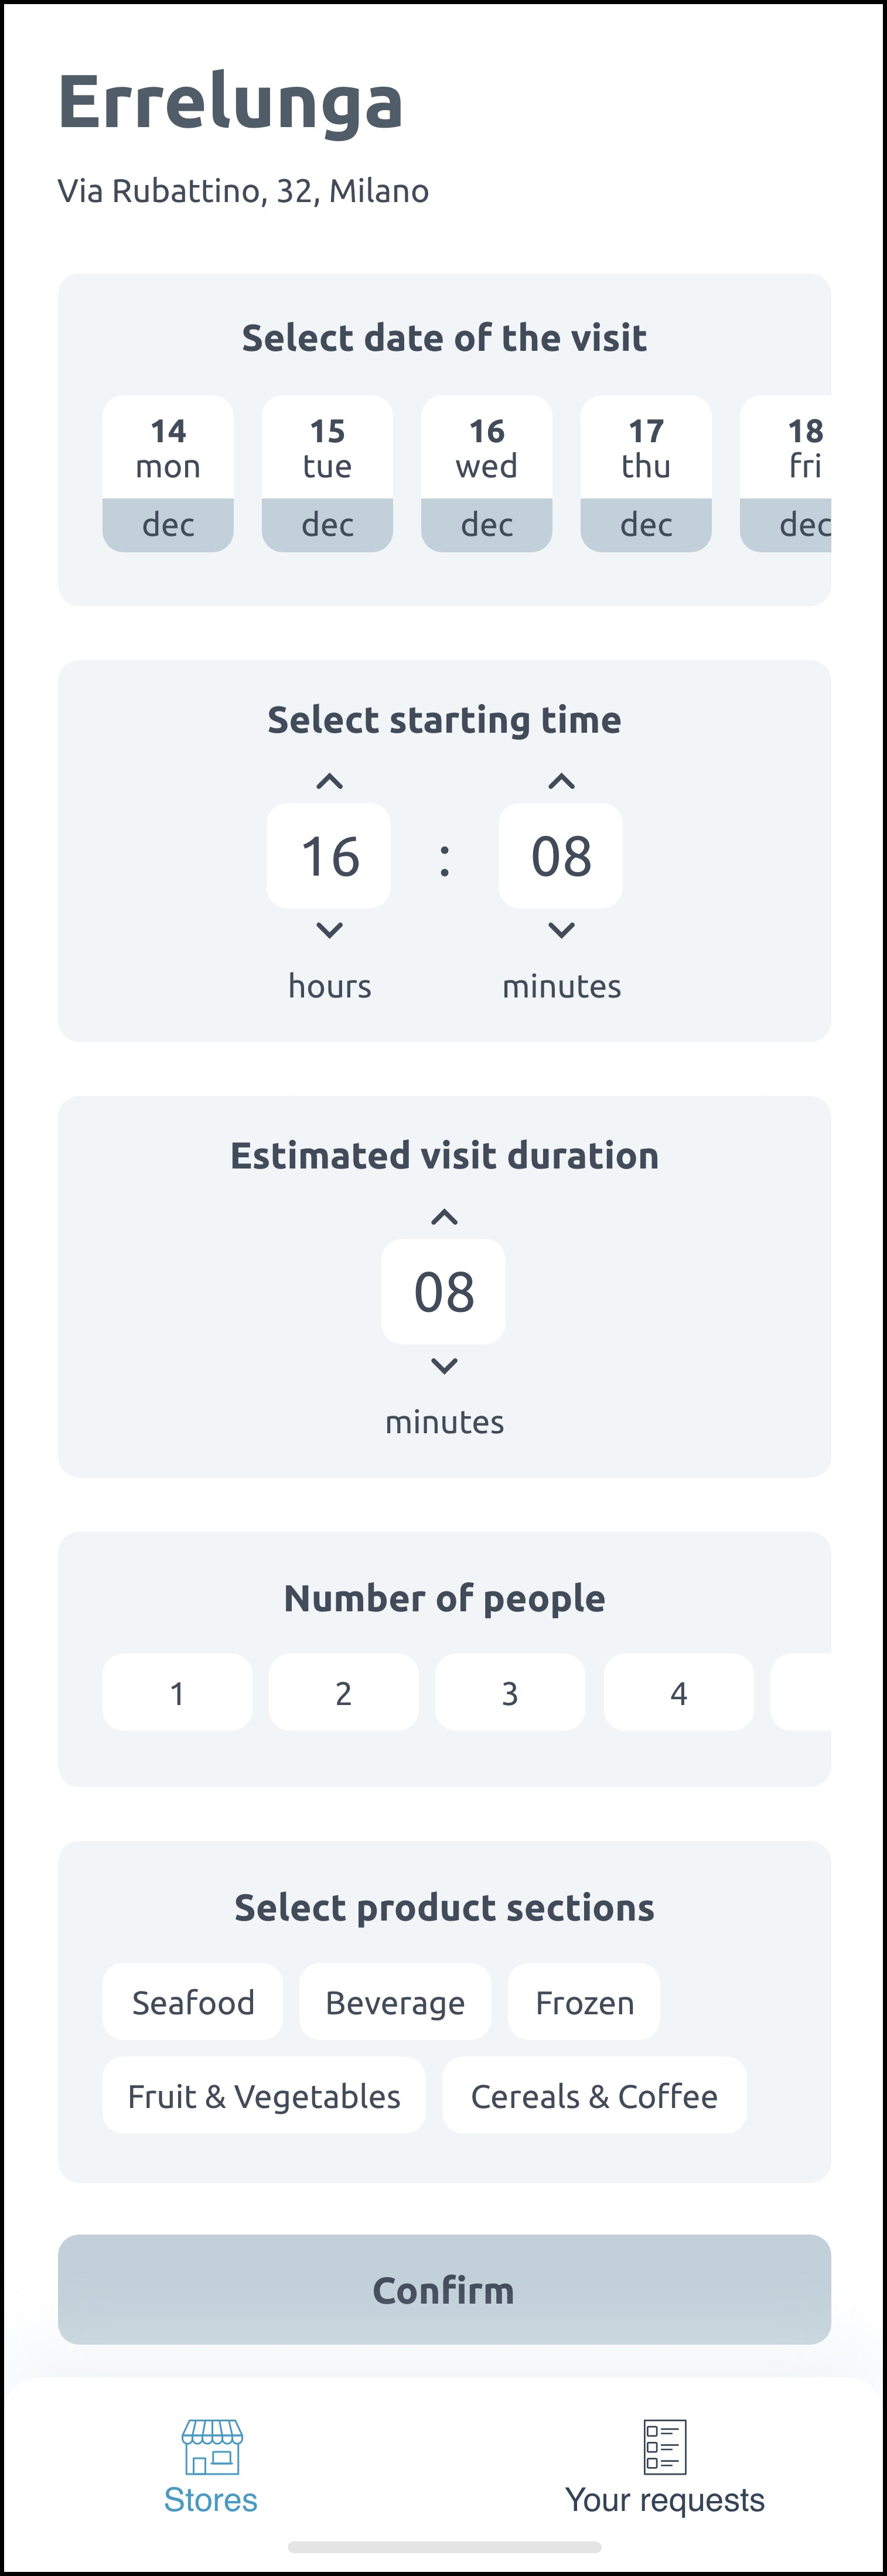
\includegraphics[width=\textwidth, height=.9\textheight, keepaspectratio]{pictures/mockups/book_a_visit}
            \captiondd{Mockup 3 -- Booking a visit for a store}{Mockup showing the form for making a booking request. It includes a button which allows to forward the request to the system. It is from the first tab of the GUI, after pressing the button ``Book a visit" of the previous mockup}
            \label{figure:mockup_3}
        \end{figure}
    \newpage
    \begin{multicols}{2}
        \begin{figure}[H]
            \centering
            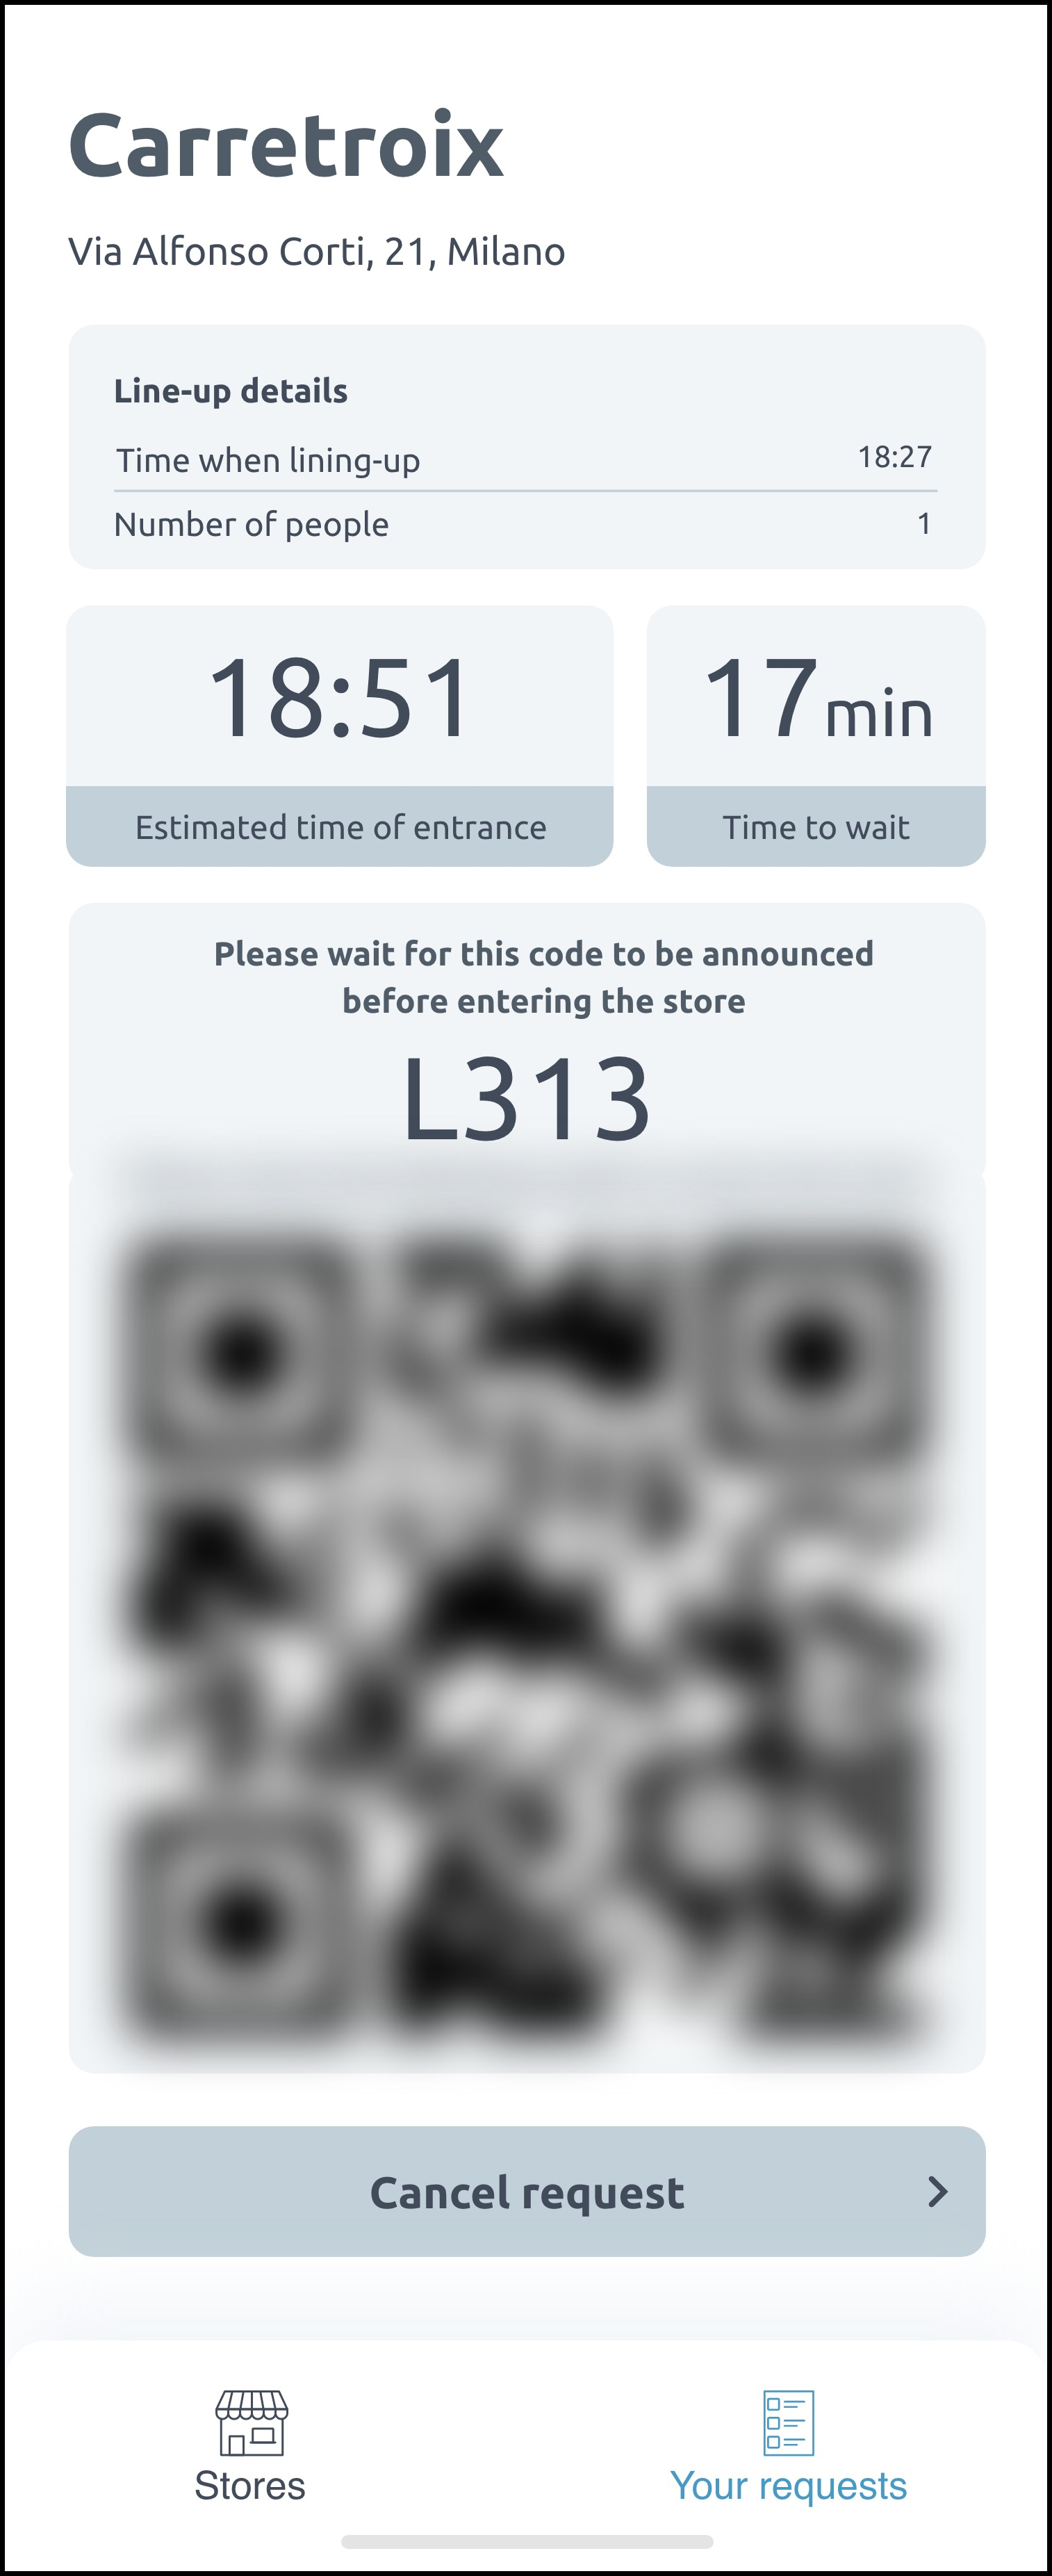
\includegraphics[width=\textwidth, height=.75\textheight, keepaspectratio]{pictures/mockups/active_line_up}
            \captiondd{Mockup 4 -- Line-up waiting to be announced}{Mockup showing the details of a pending line-up request. It includes a button which allows to cancel the request and the code identifying the request (L313). It also includes the QR code to access the store, which is blurred since the customer cannot enter yet. It is from the second tab of the GUI}
            \label{figure:mockup_4}
        \end{figure}
        \begin{figure}[H]
            \centering
            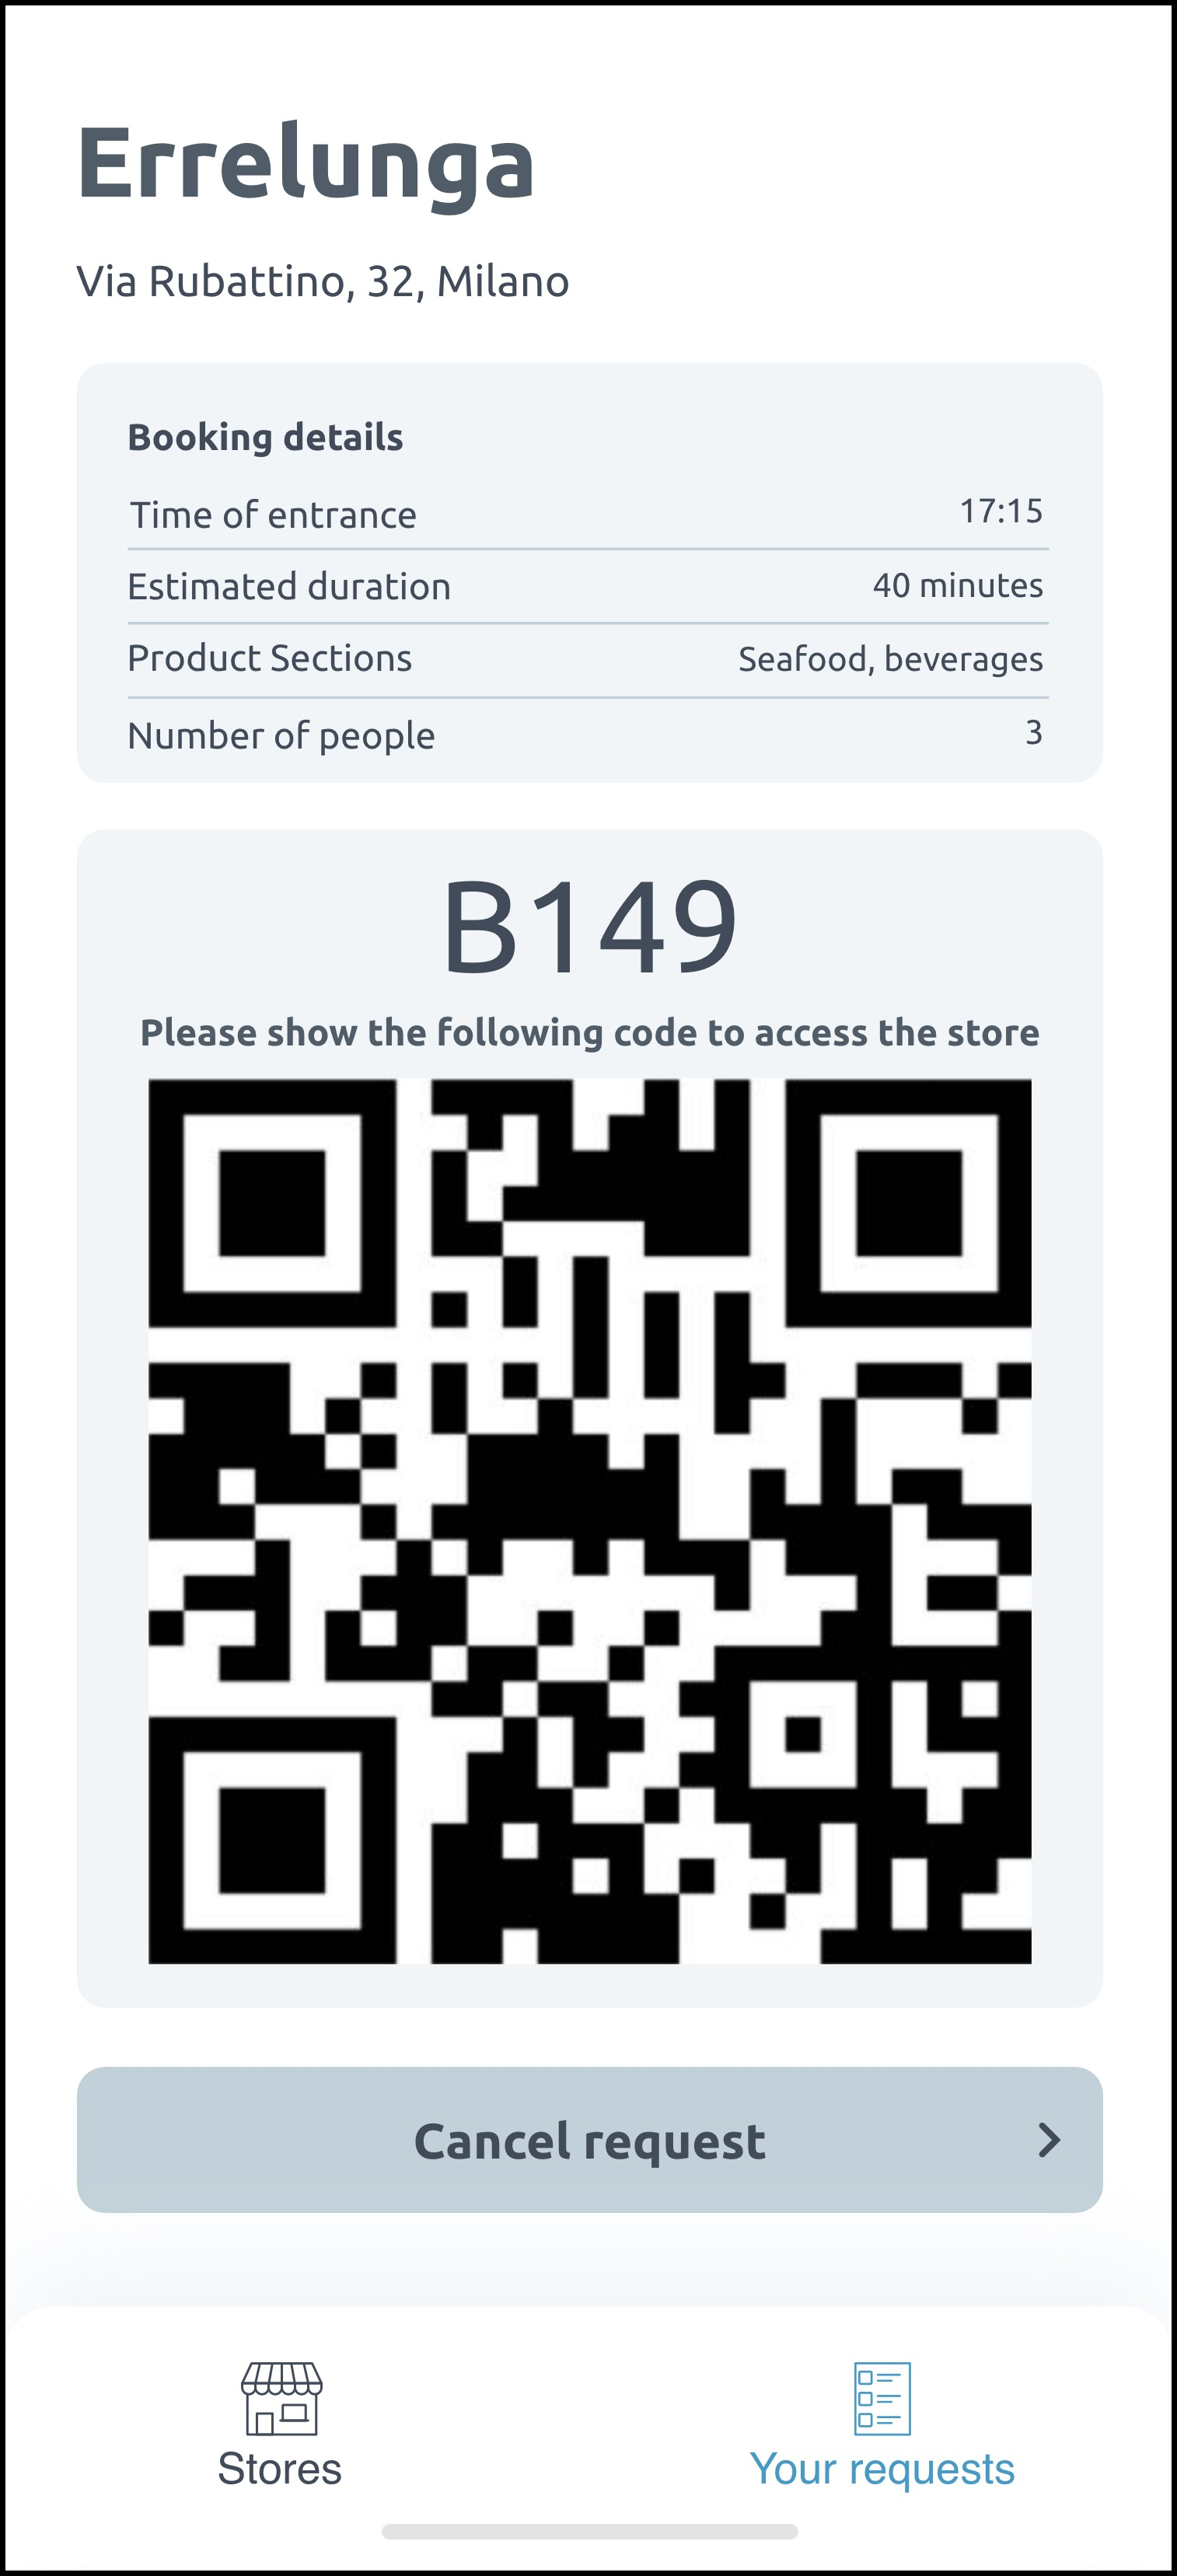
\includegraphics[width=\textwidth, height=.75\textheight, keepaspectratio]{pictures/mockups/ready_booking}
            \captiondd{Mockup 5 -- Ready booking}{Mockup showing the details of a ready booking request. It includes a button which allows to cancel the request and the code identifying the request (B149). The QR code to access the store is displayed correctly. It is from the second tab of the GUI}
            \label{figure:mockup_5}
        \end{figure}
    \end{multicols}
    \newpage
    \section{Administrative tool user interface}
    \begin{figure}[H]
            \centering
            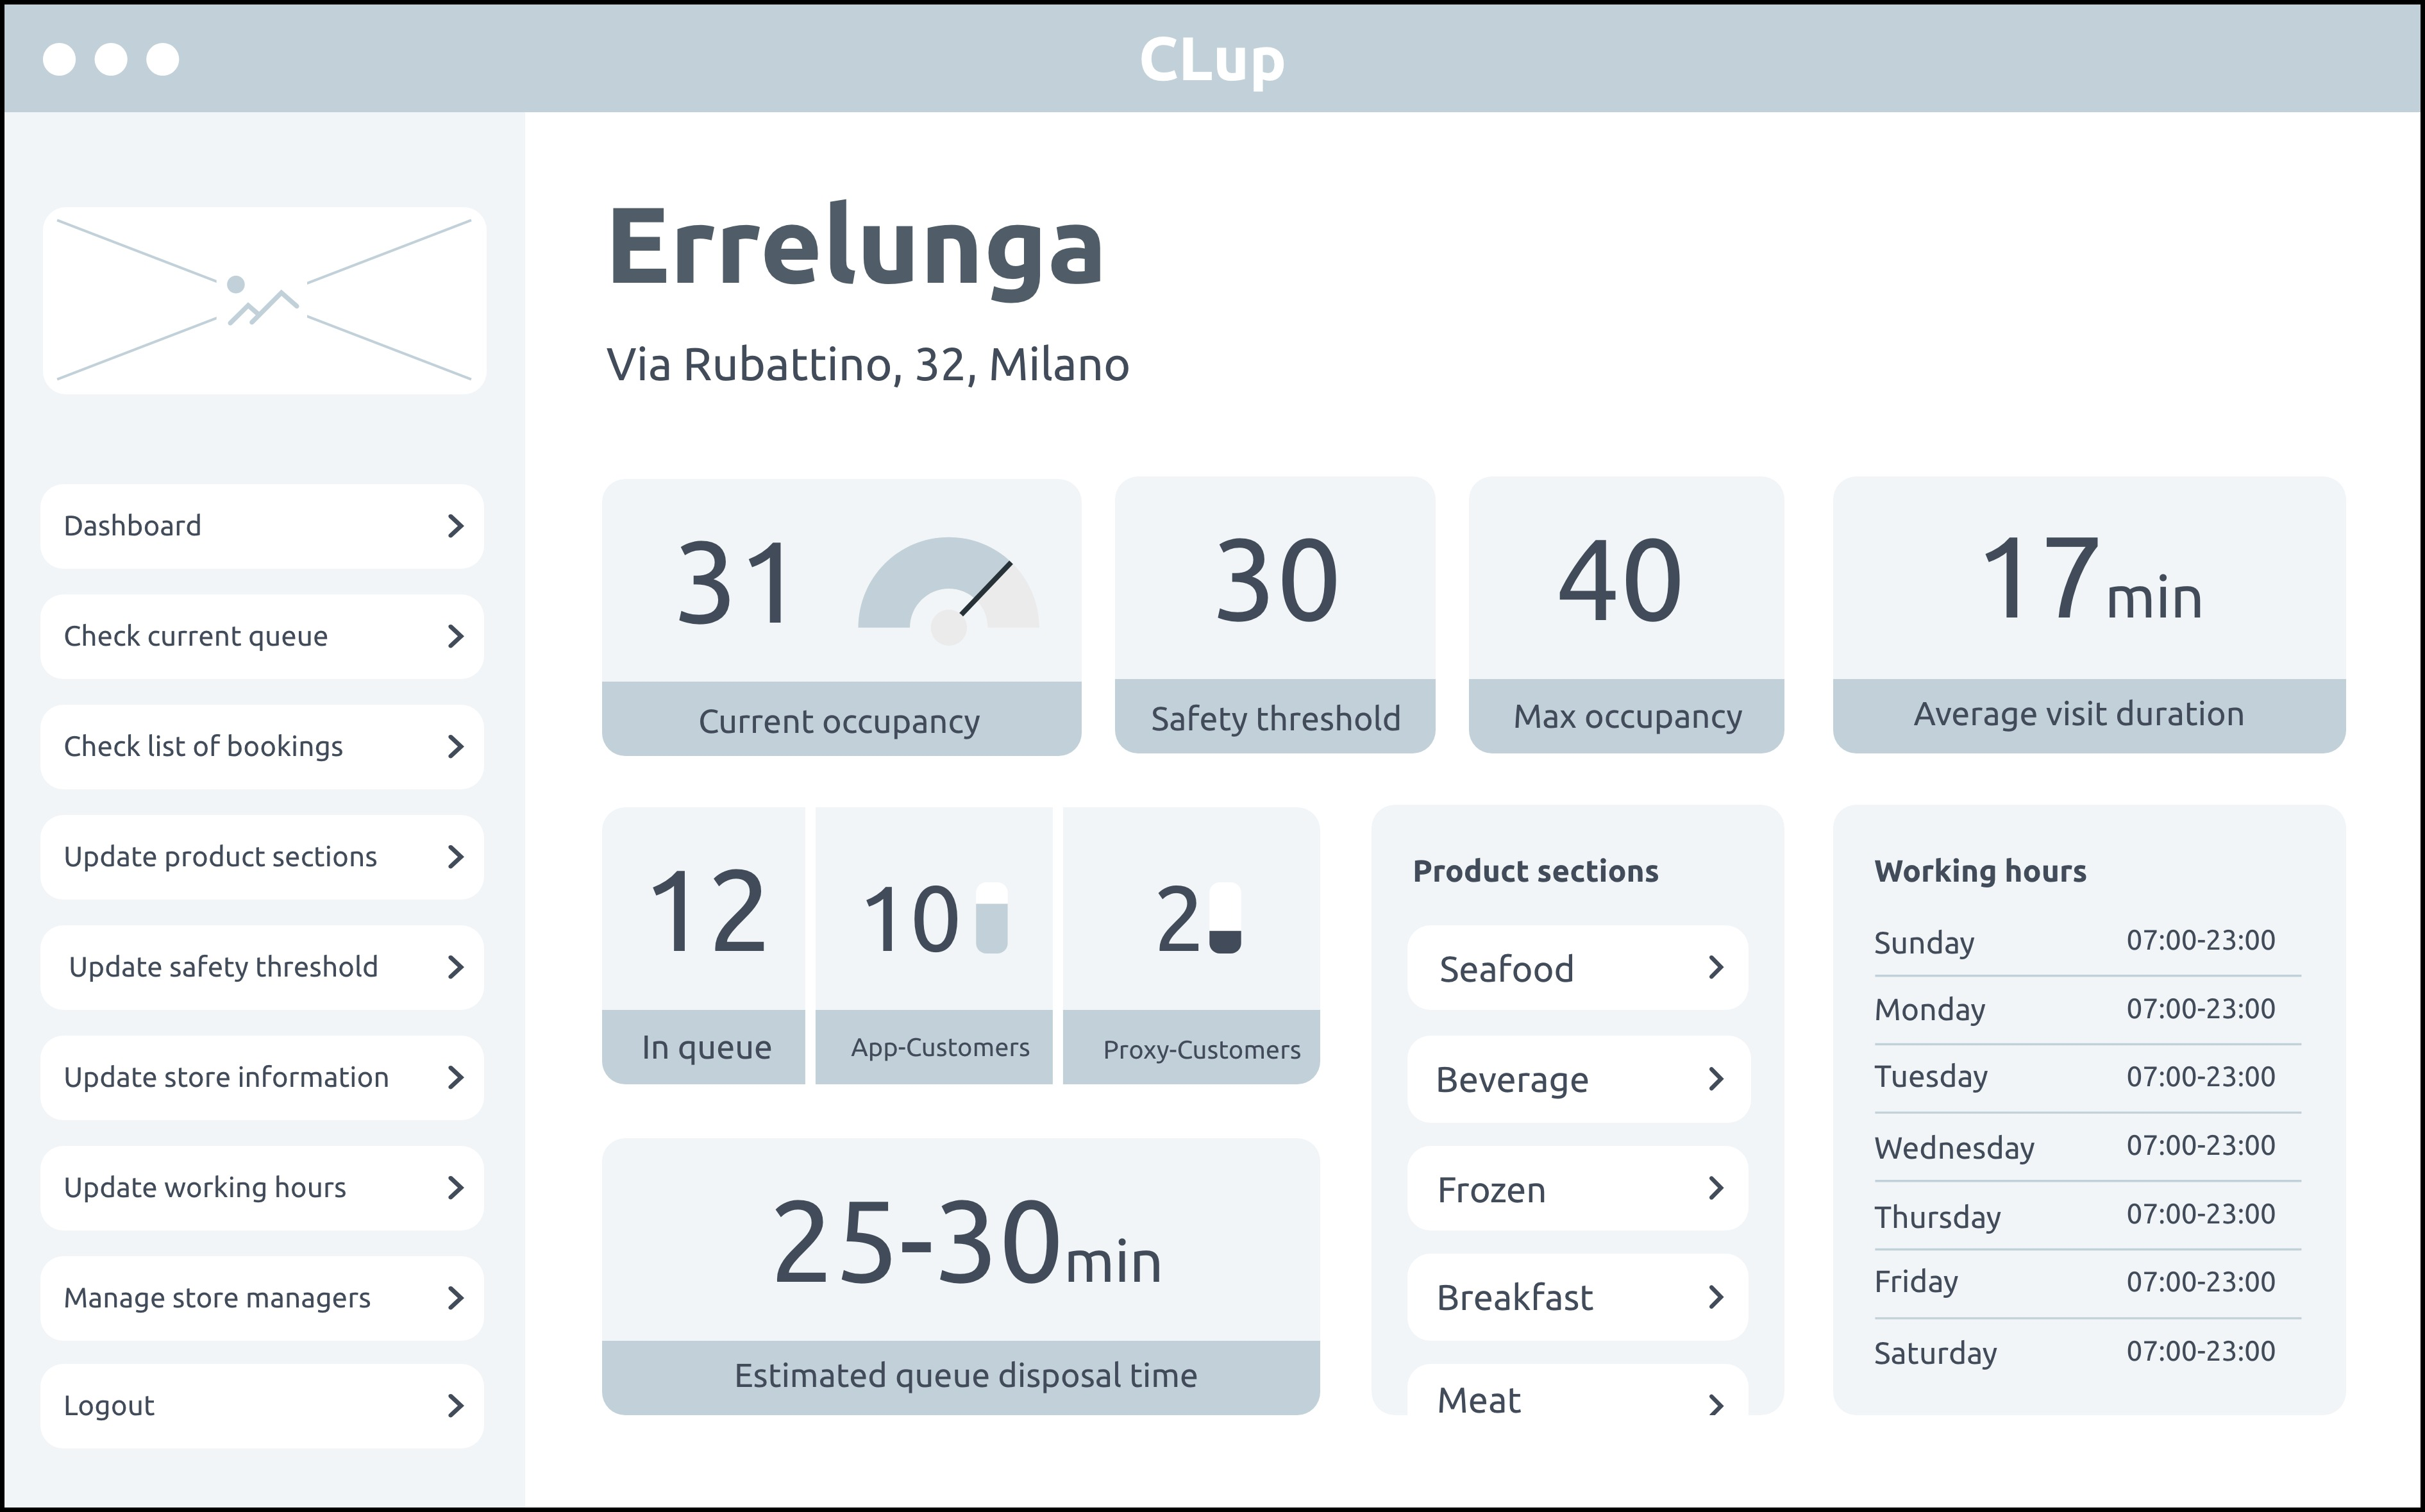
\includegraphics[width=\textwidth, keepaspectratio]{pictures/mockups/manager_view}
            \captiondd{Mockup 6 -- Store managers' administrative tool}{Mockup showing the dashboard of the administrative tool. It includes an overview of the previously selected store (from the ones administered by the manager logged in). From the left bar, it is possible to reach other pages where the manager can obtain information about the store’s queue and its active bookings or to edit its parameters and its product sections}
            \label{figure:mockup_6}
        \end{figure}
    
\chapter{Requirements traceability} 
    \begin{figure}[H]
        \centering
        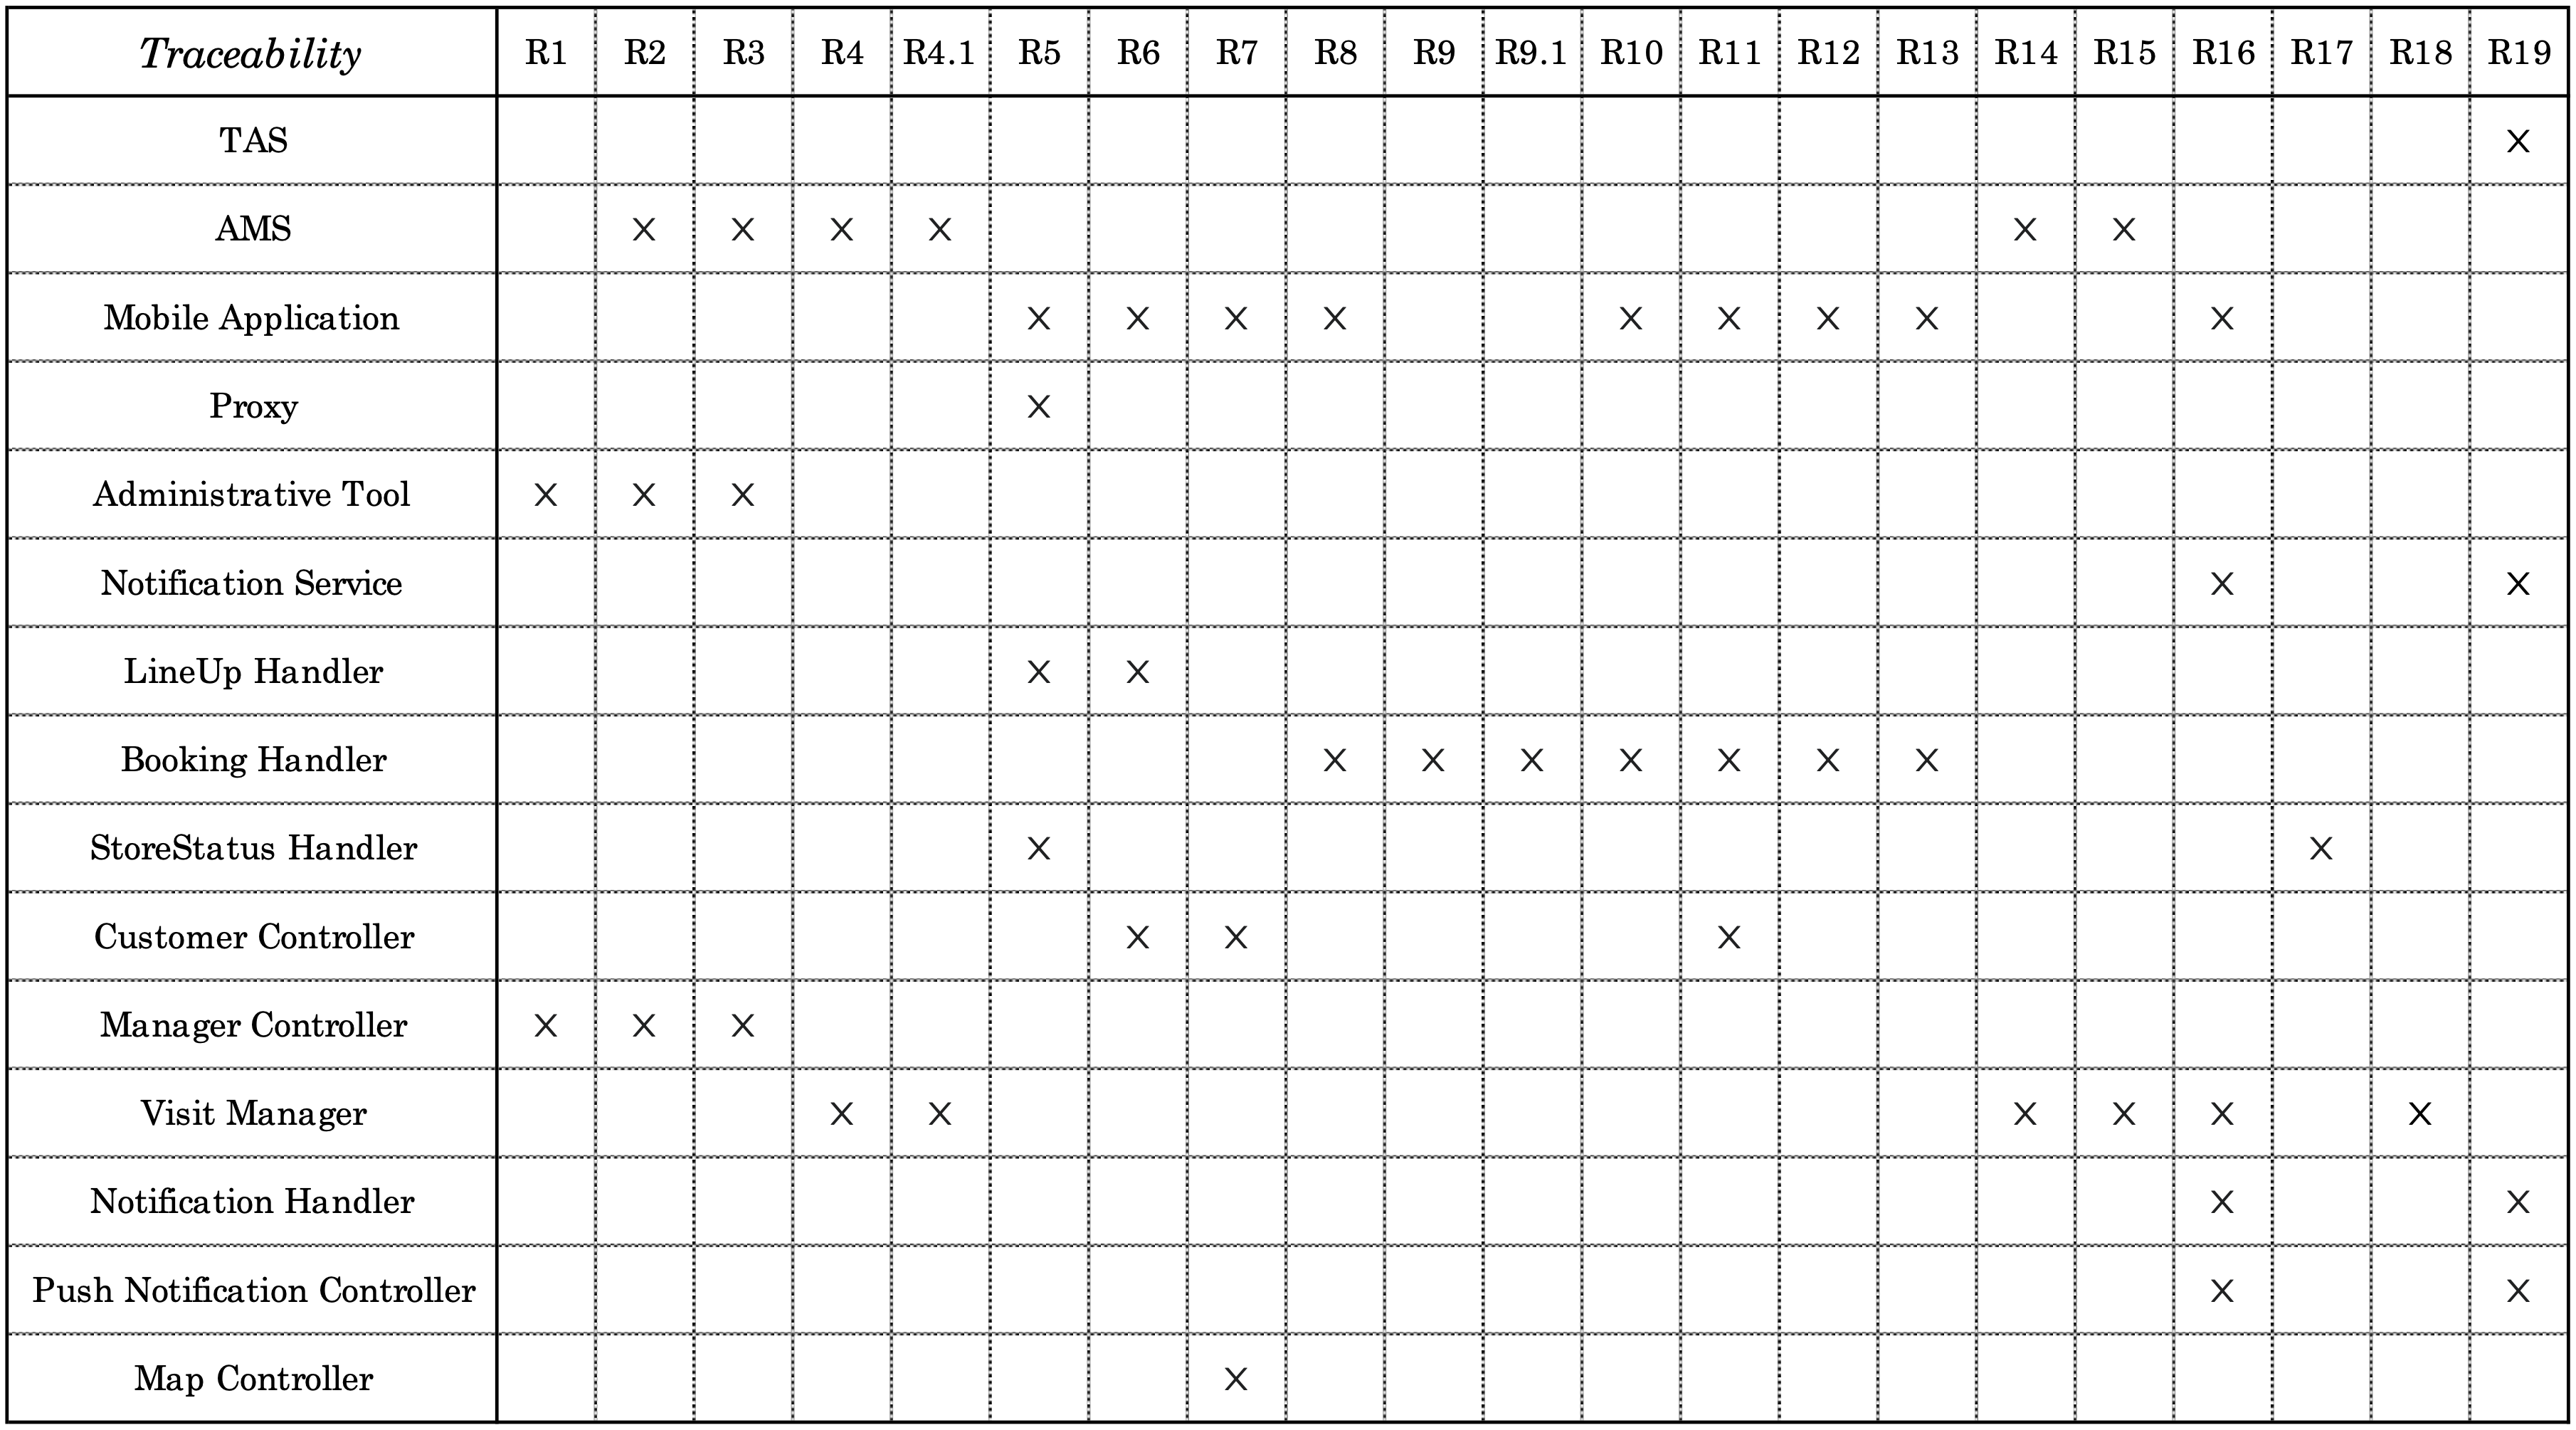
\includegraphics[width=\textwidth, height=\textheight, keepaspectratio]{pictures/traceability}
        \caption{Requirements traceability}
        \label{figure:traceabilityn}
    \end{figure}
    The DataModel and DBMS components are not indicated in the table, as they represent the data layer and all the requirements need to deal with data.

\chapter{Implementation, integration, and test plan}
    For what concerns the implementation, integration and testing, an inside-out strategy is chosen for the end-users' applications, for the server and for the DBMS. This approach, very similar to the bottom-up approach, consists in picking specific components to start the development with, and then proceed in implementing and integrating the adjacent and depending ones. \par
    In this way, while other components are developing, a subset of the system can already be integrated and tested. When the implementation of remaining components ends, only a restricted group of functionalities has still to be tested.
    \section{Implementation plan}
    The implementation of the server logic and the user applications can be carried out simultaneously by two different teams. \par
    The first implementation team, which will develop the system back-end, should begin the implementation process starting from the data-layer, choosing the DBMS to use, defining the relational schema and realizing the DataModel component, since it directly interacts with the DBMS and is the one managing all the persistent data necessary for the application to correctly and consistently work. \par
    From that moment on, the development of the other server components can be carried out in the following order. \par
    The first components to be implemented in parallel are the VisitManager and the RequestHandler. Following the inside-out implementation strategy, the development of these components has a higher priority over the remaining ones, since they cope with most of the server-side application logic. \par
    Afterwards, the attention should be focused on the implementation of the CustomerController, the ManagerController and of the StoreStatusHandler. This decision has been taken considering the role they play in allowing users to interact with the system. While the logic they implement is not of central relevance as the one implemented by the VisitManager and the Request handler, they are still needed in order to provide even the basic functionalities of CLup. \par
    The last components to be implemented are NotificationHandler, PushNotificationController, MapController. In particular, these two last components must be developed only after defining the two external services they interact with, namely the NotificationService and the MapsService. Since the functionalities they implement can be considered as advanced features that grant customers a better user experience, they can be the last components to be implemented, since their absence does not affect the correct interaction between all the other server components. \par
    A schematic division of the implementation process into phases is the following:
    \begin{enumerate}
        \item DBMS, DataModel;
        \item RequestHandler, VisitManager;
        \item CustomerController, ManagerController, StoreStatusHandler;
        \item NotificationHandler, PushNotificationController, MapController.
    \end{enumerate}
    \begin{figure}[H]
            \centering
            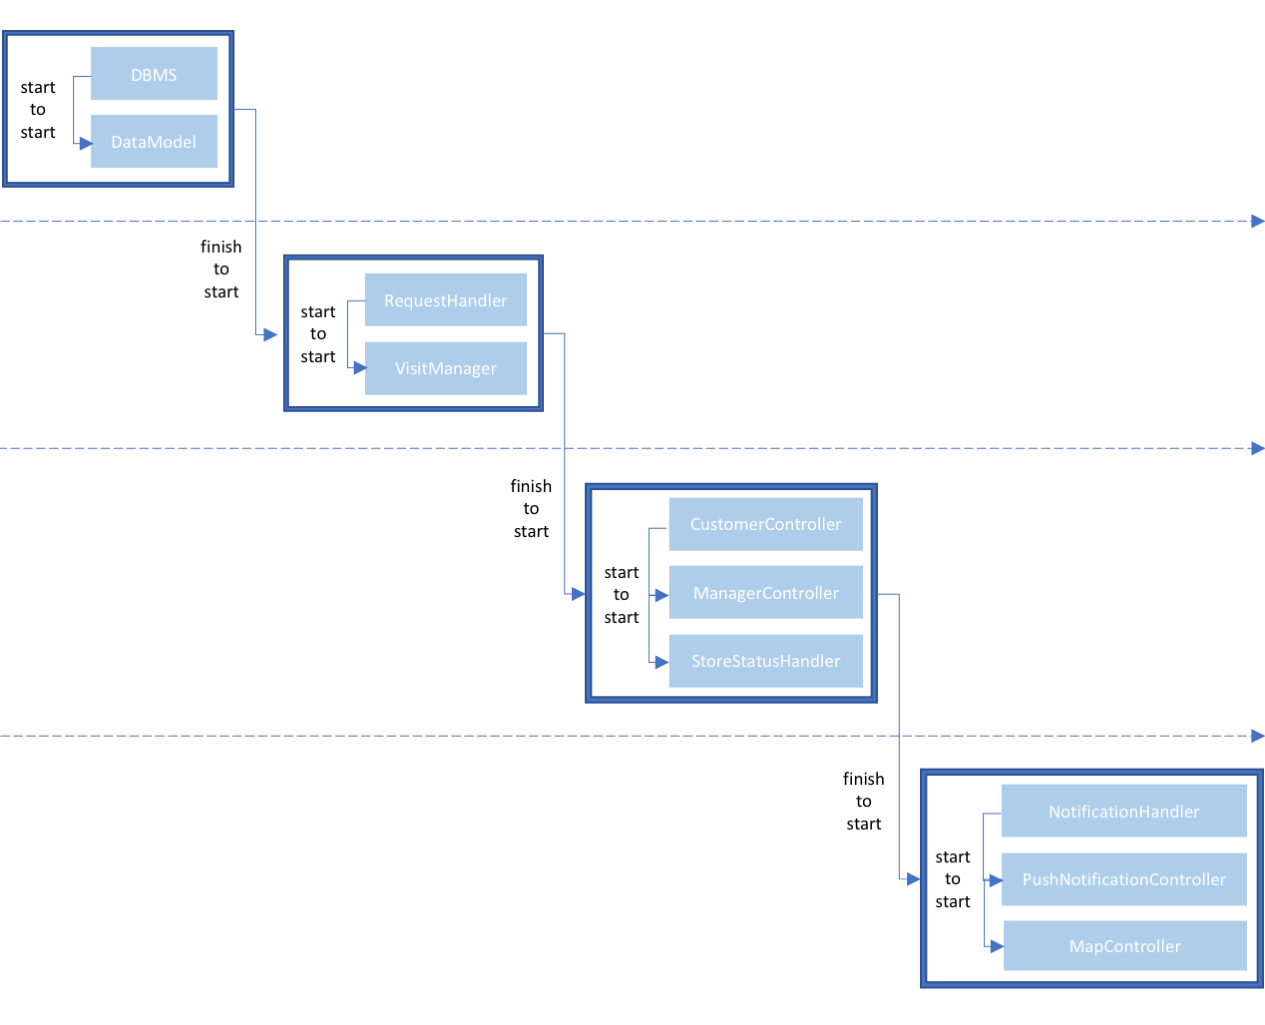
\includegraphics[width=.9\textwidth, height=\textheight, keepaspectratio]{pictures/implementation_diagram}
            \caption{Implementation diagram}
            \label{figure:implementation_diagram}
        \end{figure}
    This implementation order allows to integrate and test components in a quicker way, proceeding in ``pipeline" as soon as each implementation phase is completed. \par 
    The second implementation team, which will develop the system frontend, should be split in three different subteams, each of them implementing one of the three different user applications. Since each application is independent from the server side logic, and since communication between the server and these external components is achieved via stateless interactions, they can be implemented and tested separately, before proceeding with the final integration implementation and testing. \par
    For all the components to be implemented, accurate unit testing should be performed.
    
    \section{Integration plan}
    The integration of all the components should be done in an incremental way, exploiting the order in which they are implemented. \par
    Since the implementation begins from the data layer, the DataModel component must be accurately interfaced with the DBMS. In fact, the correctness and reliability of the integration between the DataModel and the database is fundamental for the integration of all the other components for the selected architectural pattern. In order to perform the integration testing, appropriate drivers are required. \par
    When this first integration is completely accomplished and tested, as soon as the second phase of the implementation process is over, the integration and testing of both the RequestHandler and the VisitManager should be fulfilled. Since they directly interact with the DataModel, they substitute the driver required for the previous integration test phase. However, to simulate the behaviour of the other components to be implemented, appropriate drivers are still required. Furthermore, since the VisitManager interacts with the NotificationHandler, a top-down approach is required for the specific remote notification function, which cannot be tested until this last component is fully developed. \par
    Following the implementation order, the next step of the integration phase involves the CustomerController, the ManagerController and the StoreStatusHandler components. Since all the major components of the Server are already implemented and integrated, the only required drivers to integrate and test them are the ones that simulate the users’ interaction. However, as for the VisitManager, all the functionalities that involve the NotificationHandler and the MapController cannot be integrated and tested. \par
    The last server components to be integrated with the system are the NotificationHandler, the PushNotificationHandler and the MapController, together with the external services they interact with, namely the MapsService and the NotificationService. Since the interaction between all the other server components has already been correctly integrated and tested, the only required drivers are the one which simulate the different user interactions. \par
    Once all the server components are fully integrated, the integration and testing phase should proceed integrating the presentation layer components. Thus, after each artifact is fully developed and tested, it should substitute its associated driver in the previous integration test. \par
    Eventually, when all of them are integrated, a full final functional test of the system should be performed. \par
    Since CLup requires to interact with the AccessManagementSystem, the Proxy and the TurnAnnouncementSystem of each store it manages, whenever a new store decides to benefit of CLup, the integration of those components is required, which includes a brief testing concerning their interaction with the system.
    \newpage
    \section{Other system testing}
    Once the system has passed the integration testing phase, other system tests should be performed. These tests should focus on the performance requirements and on the software system attributes specified in the Requirements Analysis and Specification Document. \par
    Thus, a first test of the system performance must be done, checking that the related requirements are satisfied. \par
    Then, adequate tests concerning the reliability and availability of the system must be performed, ensuring that the relative requirements are satisfied. Thus, an appropriate test of both the load balancer and the replicated components must be included. \par
    Finally, security tests must guarantee the required level of security. Thus, an appropriate test of the firewall must be included.
    
\chapter{Effort spent}
    All the members of the group worked mainly together, in order to guarantee consistency through the entire document. Each member of the group spent approximately 45 hours doing team working. In addition to team working, individual work has been partitioned as shown in the following tables:
    \subsubsection{Riccio Vincenzo}
    \begin{longtable}[c]{|H{.55\textwidth}|c|}
        \hline
        \textbf{Section} & {\bfseries{Hours}} \\ \hline
        \textbf{Team working} & \textbf{45} \\ \hline
        Introduction                                  & 0.5 \\ \hline
        Overview, architectural styles and patterns   & 7 \\ \hline
        Component diagrams                            & 3 \\ \hline
        Component description                         & 2 \\ \hline
        Component interfaces                          & 4 \\ \hline
        Deployment diagram                            & 1.5 \\ \hline
        Other design decisions                        & 2 \\ \hline
        Runtime views                                 & 4.5 \\ \hline
        Relevant algorithms                           & 3 \\ \hline
        User interfaces                               & 2 \\ \hline
        Requirements traceability                     & 1.5 \\ \hline
        Implementation plan                           & 1.5 \\ \hline
        Integration plan                              & 1 \\ \hline 
        Test plan                                     & 1 \\ \hline
        \caption{Effort spent -- Riccio Vincenzo}
        \label{table:effort_riccio}
    \end{longtable}
    
    \subsubsection{Sorrentino Giancarlo}
    \begin{longtable}[c]{|H{.55\textwidth}|c|}
        \hline
        \textbf{Section} & {\bfseries{Hours}} \\ \hline
        \textbf{Team working} & \textbf{45} \\ \hline
        Introduction                                  & 0.5 \\ \hline
        Overview, architectural styles and patterns   & 4 \\ \hline
        Component diagrams                            & 2 \\ \hline
        Component description                         & 4 \\ \hline
        Component interfaces                          & 2.5 \\ \hline
        Deployment diagram                            & 1.5 \\ \hline
        Other design decisions                        & 1.5 \\ \hline
        Runtime views                                 & 7 \\ \hline
        Relevant algorithms                           & 5 \\ \hline
        User interfaces                               & 2 \\ \hline
        Requirements traceability                     & 1 \\ \hline
        Implementation plan                           & 1 \\ \hline
        Integration plan                              & 1.5 \\ \hline 
        Test plan                                     & 1 \\ \hline
        \caption{Effort spent -- Sorrentino Giancarlo}
        \label{table:effort_sorrentino}
    \end{longtable}
    
    \newpage
    \subsubsection{Triuzzi Emanuele}
    \begin{longtable}[c]{|H{.55\textwidth}|c|}
        \hline
        \textbf{Section} & {\bfseries{Hours}} \\ \hline
        \textbf{Team working} & \textbf{45} \\ \hline
        Introduction                                  & 0.5 \\ \hline
        Overview, architectural styles and patterns   & 4 \\ \hline
        Component diagrams                            & 3 \\ \hline
        Component description                         & 1.5 \\ \hline
        Component interfaces                          & 3 \\ \hline
        Deployment diagram                            & 2 \\ \hline
        Other design decisions                        & 1.5 \\ \hline
        Runtime views                                 & 3.5 \\ \hline
        Relevant algorithms                           & 5 \\ \hline
        User interfaces                               & 3 \\ \hline
        Requirements traceability                     & 1 \\ \hline
        Implementation plan                           & 3 \\ \hline
        Integration plan                              & 2.5 \\ \hline 
        Test plan                                     & 1 \\ \hline
        \caption{Effort spent -- Triuzzi Emanuele}
        \label{table:effort_triuzzi}
    \end{longtable}
    
\chapter{References}
    This chapter contains references to the tools and resources used during the writing of the document. \par
    Tools:
    \begin{itemize}
        \item The UML class diagram has been designed using the software \href{https://staruml.io/}{StarUML};
        \item The sequence diagrams have been made using the software \href{https://astah.net/}{Astah};
        \item The component and deployment diagrams have been made using the software \href{https://www.visual-paradigm.com/}{Visual Paradigm}.
    \end{itemize}
    Other resources:
    \begin{itemize}
        \item Restful APIs: \par \small{\url{https://restfulapi.net/}}
        \item Tier vs layer: \par \small{\url{https://www.ibm.com/cloud/learn/three-tier-architecture/}}
        \item Worldwide mobile and desktop market share: \par \small{\url{https://gs.statcounter.com}}
        \item Martin Fowler's repository pattern: \par \small{\url{https://martinfowler.com/eaaCatalog/repository.html}}
    \end{itemize}

\listoftables
\listoffigures

\end{document}